\documentclass[12pt, a4paper]{report}

% --- UNIVERSAL PREAMBLE BLOCK ---
% Margins: Left = 1.5 inch, Right = 1 inch, Top = 1 inch, Bottom = 1 inch
\usepackage[a4paper, top=1in, bottom=1in, left=1.5in, right=1in]{geometry}
\usepackage{fontspec}

\usepackage[english, bidi=basic, provide=*]{babel}
\babelprovide[import, onchar=ids fonts]{english}
\babelfont{rm}{Times New Roman}

% --- OTHER REQUIRED PACKAGES ---
% REMOVE the '[demo]' option below when you upload your actual images to Overleaf. 
% 'demo' renders all \includegraphics commands as black placeholder boxes to prevent errors.
\usepackage{graphicx} 
\usepackage{subcaption} % Required for 2x2 image grids
\usepackage{mdframed}   % Required for the framed GitHub box
\usepackage{tcolorbox}
\usepackage{tikz} % for drawing diagrams and flowchart.
\usetikzlibrary{shapes.geometric, arrows.meta, positioning}

\usepackage{setspace} % For line spacing
\onehalfspacing % Sets 1.5 line spacing globally

\usepackage{fancyhdr} % For simple and clean headers
\usepackage{amsmath, amssymb, amsfonts} % For mathematical foundations and equation placeholders
\usepackage{titlesec} % For professional chapter title formatting
\usepackage{xcolor} % For colors in code listings
\usepackage{listings} % For code placeholders
\usepackage{booktabs} % For professional tables
\usepackage{hyperref} % Always load hyperref last
\usepackage{pdfpages} % Required for inserting external page PDFs

% --- HYPERREF SETUP ---
\hypersetup{
    colorlinks=true,
    linkcolor=black, % Keep it professional and black for printing
    filecolor=black,      
    urlcolor=blue,
    citecolor=black,
    pdftitle={A Python-Based Approach to Animate Geometry and Data},
    pdfauthor={Shubham Tiwari}
}

% --- WATERMARK SETUP ---
% \usepackage{draftwatermark}
% \SetWatermarkText{\shortstack{Copyright \copyright\ Shubham Tiwari \\ Read Only Specimen}}
% \SetWatermarkColor[gray]{0.85} % Light gray so you can still read the math
% \SetWatermarkScale{0.8}
% \SetWatermarkAngle{45}

% --- CODE LISTING SETUP (Python Style) ---
\lstset{
    language=Python,
    basicstyle=\ttfamily\small,
    keywordstyle=\color{blue}\bfseries,
    stringstyle=\color{red},
    commentstyle=\color{green!50!black},
    numbers=left,
    numberstyle=\tiny\color{gray},
    stepnumber=1,
    frame=single,
    breaklines=true,
    captionpos=b
}

% --- HEADER AND FOOTER SETUP ---
\pagestyle{fancy}
\fancyhf{} % Clear all header and footer fields
\fancyhead[R]{\nouppercase{\leftmark}} % Right header: Chapter name
\fancyfoot[C]{\thepage} % Center footer: Page number
\renewcommand{\headrulewidth}{0.5pt} % Simple clean line under header

% --- CHAPTER TITLE FORMATTING ---
\titleformat{\chapter}[display]
  {\normalfont\huge\bfseries}{\chaptertitlename\ \thechapter}{20pt}{\Huge}
\titlespacing*{\chapter}{0pt}{-20pt}{40pt}

\begin{document}

% ==============================================================================
% FRONTMATTER (Roman Numerals)
% ==============================================================================
\pagenumbering{roman}

% ------------------------------------------------------------------------------
% 1. COVER PAGE (Matches DU/Dyal Singh Format)
% ------------------------------------------------------------------------------
\begin{titlepage}
    \centering
    % Placeholder for college logo
    
\includegraphics[width=5cm]{college_logo.png}\\[0.5cm]
 
    {\Huge \textbf{A Python-Based Approach to Animate Geometry and Data}}\\[1cm]
    
    {\normalsize \textbf{Project work Submitted for the}}\\[0.2cm]
    {\normalsize \textbf{Award of the Degree of}}\\[0.2cm]
    {\normalsize \textbf{Bachelor of Science (Hons.) in}}\\[0.2cm]
    {\normalsize \textbf{Mathematics}}\\[1cm]
   
    {\normalsize \textbf{By}}\\[0.2cm]
    {\Large \textbf{Shubham Tiwari}}\\[0.2cm]
    {\normalsize Semester VIII}\\[1cm]
    
    {\normalsize \textbf{Department of Mathematics}}\\[0.2cm]
    {\normalsize \textbf{Dyal Singh College}}\\[0.2cm]
    {\normalsize \textbf{(University of Delhi)}}\\[0.2cm]
    {\normalsize \textbf{Lodhi Road}}\\[0.2cm]
    {\normalsize \textbf{New Delhi-110003}}\\[0.5cm]
    
    {\normalsize \textbf{April 2026}}
\end{titlepage}

\clearpage

% ------------------------------------------------------------------------------
% 2. TITLE PAGE (Duplicate of Cover Page but counted as page ii)
% ------------------------------------------------------------------------------
\begin{titlepage}
    \centering
    
\includegraphics[width=5cm]{college_logo.png}\\[0.5cm]
    
    {\huge \textbf{A Python-Based Approach to Animate Geometry and Data}}\\[0.8cm]
    
    {\normalsize \textbf{Project work Submitted for the}}\\[0.2cm]
    {\normalsize \textbf{Award of the Degree of}}\\[0.2cm]
    {\normalsize \textbf{Bachelor of Science (Hons.) in}}\\[0.2cm]
    {\normalsize \textbf{Mathematics}}\\[0.8cm]
    
    {\normalsize \textbf{By}}\\[0.2cm]
    {\Large \textbf{Shubham Tiwari}}\\[0.5cm]
    
    \begin{flushleft}
    \small
    \textbf{Supervisor:}\\
    Dr. J. V. Ramani\\
    Department of Mathematics\\[0.3cm]
    
    \textbf{Co-Supervisor:}\\
    Ms. Ishver Rani Manchanda\\
    Department of Mathematics
    \end{flushleft}
    \vfill
    
    {\normalsize \textbf{Department of Mathematics}}\\[0.2cm]
    {\normalsize \textbf{Dyal Singh College}}\\[0.2cm]
    {\normalsize \textbf{(University of Delhi)}}\\[0.2cm]
    {\normalsize \textbf{New Delhi-110003}}\\[0.2cm]
    {\normalsize \textbf{2026}}
\end{titlepage}

\clearpage

% ------------------------------------------------------------------------------
% 3. SUPERVISOR CERTIFICATE
% ------------------------------------------------------------------------------
\chapter*{Certificate}
\addcontentsline{toc}{chapter}{Certificate}

\begin{center}
    \textbf{CERTIFICATE}
\end{center}

\vspace{1cm}
I am satisfied that the project work presented by \textbf{Shubham Tiwari} entitled \textbf{``A Python-Based Approach to Animate Geometry and Data''} is worthy of consideration for the award of the degree of Undergraduate Degree with research.

\vspace{0.5cm}
I certify that:
\begin{enumerate}
    \item[(a)] He has pursued the prescribed course of research.
    \item[(b)] He is of good moral character.
\end{enumerate}

\vspace{3cm}

\begin{minipage}[t]{0.45\textwidth}
\begin{flushleft}
    \textbf{Supervisor}\\
    Dr. J. V. Ramani\\
    Department of Mathematics\\
    Dyal Singh College\\
    Email: \\
    Mob. No: 
\end{flushleft}
\end{minipage}
\hfill
\begin{minipage}[t]{0.45\textwidth}
\begin{flushleft}
    \textbf{Co-Supervisor}\\
    Ms. Ishver Rani Manchanda\\
    Department of Mathematics\\
    Dyal Singh College\\
    Email: \\
    Mob. No: 
\end{flushleft}
\end{minipage}

\vspace{3cm}
\begin{center}
    \textbf{Countersigned}\\[1.5cm]
    \textbf{Head of the Department}\\
    Department of Mathematics\\
    Dyal Singh College
\end{center}

\clearpage

% ------------------------------------------------------------------------------
% 4. DECLARATION PAGE
% ------------------------------------------------------------------------------
\chapter*{Declaration}
\addcontentsline{toc}{chapter}{Declaration}

To,\\[0.2cm]
The Principal\\
Dyal Singh College\\
University of Delhi\\
New Delhi-110003

\vspace{1cm}
\textbf{Sir,}

\vspace{0.5cm}
I have been pursuing a course of research as a student of this College and now I want to apply for submission of my project work for the award of my degree. The relevant documents are attached herewith.

\vspace{0.5cm}
Yours faithfully,

\vspace{2cm}
\textbf{Signature:} \hrulefill\\[0.5cm]
\textbf{Name in full:} Shubham Tiwari\\[0.5cm]
\textbf{Dated:} \hrulefill\\[0.5cm]
\textbf{Address:} \hrulefill\\[0.5cm]
\textbf{Tele. No. / Mob. No.:} \hrulefill

\clearpage

% ------------------------------------------------------------------------------
% 5. CERTIFICATE OF ORIGINALITY
% ------------------------------------------------------------------------------
\chapter*{Certificate of Originality}
\addcontentsline{toc}{chapter}{Certificate of Originality}

\begin{center}
    
\includegraphics[width=3cm]{college_logo.png}\\[0.5cm]
    {\large GATHER YE THE WISDOM OF EAST AND WEST}\\[0.5cm]
    {\Large \textbf{DYAL SINGH COLLEGE}}\\[0.5cm]
    {\large \textbf{Department of Mathematics}}\\[0.5cm]
    {\large \textbf{New Delhi-110003}}\\[1cm]
    {\Large \textbf{Certificate of Originality}}\\[1cm]
\end{center}

\begin{flushright}
    \textbf{Date:} \hrulefill
\end{flushright}

\vspace{1cm}
The research work embodied in this Project entitled \textbf{``A Python-Based Approach to Animate Geometry and Data''} has been carried out by me at the Department of Mathematics, Dyal Singh College, University of Delhi, Delhi, India. 

\vspace{0.5cm}
The manuscript has been subjected to plagiarism check by software. The work submitted for consideration of award of B.Sc. (Hons.) Mathematics degree is original.

\vspace{3cm}

\begin{flushright}
    \textbf{Name and Signature of the Candidate}\\
    Shubham Tiwari
\end{flushright}

\clearpage

% ------------------------------------------------------------------------------
% 6. PLAGIARISM VERIFICATION PAGE
% ------------------------------------------------------------------------------
\chapter*{Plagiarism Verification Report}
\addcontentsline{toc}{chapter}{Plagiarism Verification Report}

\begin{center}
    
\includegraphics[width=3cm]{college_logo.png}\\[0.5cm]
    {\large GATHER YE THE WISDOM OF EAST AND WEST}\\[0.5cm]
    {\Large \textbf{DYAL SINGH COLLEGE}}\\[0.5cm]
    {\large \textbf{UNIVERSITY OF DELHI}}\\[1cm]
    {\Large \textbf{Plagiarism Verification Report}}\\[1cm]
\end{center}

\noindent \textbf{Title of the Dissertation:} A Python-Based Approach to Animate Geometry and Data\\[0.3cm]
\textbf{Research Scholar:} Shubham Tiwari\\[0.3cm]
\textbf{Supervisor:} Dr. J. V. Ramani\\[0.3cm]
\textbf{Co-Supervisor:} Ms. Ishver Rani Manchanda\\[0.3cm]
\textbf{Department:} Mathematics\\[0.3cm]
\textbf{Faculty:} Science\\[0.3cm]
\textbf{Date:} \hrulefill\\[0.3cm]
\textbf{Total Pages:} \hrulefill\\[0.5cm]

\noindent This is to report that the above project work was scanned for similarity detection. Process and outcome are given below:

\vspace{0.5cm}
\noindent \textbf{Software used:} Turnitin\\[0.3cm]
\textbf{Date:} 01-May-2026\\[0.3cm]
\textbf{Similarity Index:} 2\%\\[0.3cm]
\textbf{Total word count:} 6768\\[0.5cm]

\noindent The complete report of the above project has been forwarded to the College.

\vspace{3cm}
\begin{flushright}
    \textbf{Checked by}\\
    \textbf{Name \& Signature}
\end{flushright}

\clearpage

% ------------------------------------------------------------------------------
% 7. AI USAGE DECLARATION
% ------------------------------------------------------------------------------
\chapter*{AI Usage Declaration}
\addcontentsline{toc}{chapter}{AI Usage Declaration}

This is to declare that while AI language models were utilized as supplementary assistants—primarily to improve grammar, assist with LaTeX formatting, and debug minor Python issues—the core mathematical logic, Python code, visualizations, and intellectual property remain entirely original. 

In full compliance with institutional rules, the foundational algorithms and main research findings of this report were developed independently. Furthermore, the accompanying \textbf{Turnitin} AI Writing Overview report confirms that \textbf{0\%} of the qualifying text is detected as AI-generated.

\clearpage


% ------------------------------------------------------------------------------
% 8. ACKNOWLEDGEMENT
% ------------------------------------------------------------------------------
\chapter*{Acknowledgement}
\addcontentsline{toc}{chapter}{Acknowledgement}

I would like to express my deepest gratitude to my supervisor, Dr. J. V. Ramani, for his constant support, guidance, and encouragement throughout my project. He constantly guided me and was an invaluable mentor during this project. His extensive knowledge and support helped a lot. Through his understanding and experience, it helped me learn mathematical theory and computer programming. 

I owe my gratitude to my co-supervisor, Ms. Ishver Rani Manchanda, for her insightful feedback, technical assistance, and continuous motivation during the development of this framework. 

Moreover, I will also thank the Dyal Singh College's Department of Mathematics, University of Delhi, for their assistance and providing an environment conducive to academic investigation. Lastly, I thank my family and friends with a warm heart for being patient and encouraging throughout the process of bringing these mathematical animations to life.

\clearpage

% ------------------------------------------------------------------------------
% 9. ABSTRACT
% ------------------------------------------------------------------------------
\chapter*{Abstract}
\addcontentsline{toc}{chapter}{Abstract}

This project presents a strong computational framework in Python designed to convert static geometric equations and mathematical data into dynamic and interactive animations. Students should focus on visualizing abstract mathematical concepts in their thinking, making theoretical concepts easier to visualize and understand. 

Through the use of Python's powerful scientific ecosystem, the project employs NumPy for vectorized arrays, heavy data processing, and linear algebra. It creates a standardized pipeline for programmatic animation. The implementation proceeds from basic 2D kinematics, like parametric curves and random movements, to sophisticated 3D shapes. The use of $SO(3)$ rotation matrices reveals the topological morphing of $L_p$ norm spaces and acts as a catalyst in the implementation of differential geometry concepts. These include minimal surfaces such as the catenoid, helicoid, and Boy's surface. 

The project demonstrates that by converting continuous mathematical domains, appropriate programmatic animation may increase student engagement. We should relate mathematical concepts to student experience as far as possible to improve the understanding of mathematics.

\clearpage

% ------------------------------------------------------------------------------
% 10. TABLE OF CONTENTS, FIGURES, TABLES, SYMBOLS
% ------------------------------------------------------------------------------
\tableofcontents
\clearpage

\listoffigures
\clearpage

\listoftables
\clearpage

\chapter*{List of Symbols / Notation}
\addcontentsline{toc}{chapter}{List of Symbols / Notation}
% USER INSTRUCTION: Add your mathematical symbols here.
\begin{tabbing}
    \hspace*{3cm} \= \kill
    $x, y, z$ \> Cartesian Coordinates \\
    $\theta, \phi$ \> Angular parameters (Azimuth, Elevation) \\
    $R_{z}(\theta)$ \> Rotation matrix about the z-axis \\
    $||x||_p$ \> $L_p$ Norm \\
    $\mathbb{R}^3$ \> 3-Dimensional Euclidean Space
\end{tabbing}

\clearpage

% ==============================================================================
% MAIN REPORT STRUCTURE (Arabic Numerals)
% ==============================================================================
\pagenumbering{arabic}

% ------------------------------------------------------------------------------
% CHAPTER 1: INTRODUCTION
% ------------------------------------------------------------------------------
\chapter{Introduction}
% USER INSTRUCTION: 
% - write project motivation here
% - explain mathematics visualization problem
% - explain importance of animation
% - explain educational value
% - explain why Python was chosen

\section{Project Motivation}

Since childhood, we have all been learning Mathematics—from basic counting and drawing shapes to addition, multiplication, and tables. Remember how our parents and teachers taught us these topics? They would often say, ``Beta, assume we have 10 ice creams. If you eat 4 of them, how many are left?'' We would then count on our fingers and answer, ``six.'' Our creative minds would naturally visualise that scenario to find the answer. As we grew older, we tried to learn and visualise more. However, it became harder to understand advanced mathematical concepts, as topics like trigonometry often started going above our heads. There are many reasons why we gradually lose interest in Mathematics—such as teachers not presenting the subject engagingly, or students becoming bored during lectures and looking outside the classroom window. Whatever the reason may be, one thing is clear: we slowly lose interest in the subject.

But what if we started including animations and visualisation in Mathematics? What if we could see how derivatives work, how integration works, and how areas are broken down into small rectangular pieces and then combined again (of course, by taking the width of each rectangle close to zero) to obtain the final area? What if we could see how mathematical functions actually work—like machines that take input from one side and produce output from the other? What if we could visualise how a function's domain looks and how its codomain appears?

What if we could actually see all the things we are learning? One may ask, ``Is it possible to visualise all of Mathematics?'' Of course, this question naturally arises because Mathematics is often considered highly abstract in nature.

\section{The Mathematics Visualization Problem}

The answer to the previous question is \textbf{YES!} Mathematics can be visualised because, in many ways, it reflects patterns found in nature. I remember a quote from one of the brilliant mathematicians and \textit{Fields Medal} winners, \textbf{William Thurston}:

\begin{tcolorbox}[colback=gray!5!white, colframe=black!75!white, title=Quote]
\textit{``I think that the most important thing a mathematician can do is to show that mathematics is a human activity, not some supernatural fictional world, and that it is one of the most creative fields.''}
\end{tcolorbox}

This is what many students are unable to experience. We learn theorems and memorise proofs, but if someone asks about the intuition or logic behind them, students often remain silent because they lack a strong conceptual understanding of the topic. This is where visualisation becomes important.

For example, there is a beautiful subject called Differential Geometry, which studies curves and surfaces. In many cases, teachers ask students to memorise parametrisation equations for these surfaces. However, I believe the most important aspect is to actually see how these shapes are formed—how mathematics and coding work together to create visual structures and bring these shapes to life.

Thus, the gap between theory and building strong intuition is what this project is trying to fill.


\section{The Importance of Animation in Education}

Animations of math concepts make learning more fun and interactive. I have taught students in tuition classes and once tried to explain trigonometry using only theoretical explanations. However, they had trouble understanding and often said, "Sir, kuch samajh nahi aa raha, kya yeh itna hard subject hai?" I realized that this was the wrong way to go because students may lose interest in the subject if they don't build intuition.

I didn't just tell them that $\sin \theta = \frac{P}{H}$, I showed them a triangle and let them try out different side lengths. By looking and exploring, they found that there was always a constant relationship. I then told them that this constant relationship is what we call sine. After they saw the graph of the sine function, they started to understand how sine and other trigonometric ratios repeat.

This shows how using animation and visualization can make learning faster, clearer, and more fun.

In today's rapidly changing world, a traditional approach won't work easily. Teachers must upgrade their teaching methods, and students should also make an effort to develop a deeper understanding by visualizing concepts. When these students become teachers themselves, they can pass this knowledge more interactively and intuitively. This helps create genuine learners rather than students who simply memorize information like parrots.


\section{Why Python?}
 One of the genuine question arises:  why not we go and use built in software for mathematical animation such as \textbf{Geogebra}, I say its good, but learning the process from scratch, gives you different feeling, and also note that these software have only have finite set of animations, and if someone ask why not \textbf{C++}, or any other language, the reason is simple!, The easiness of \textbf{Python}, is what makes it great that even non-programmers would also start doing coding, after learning that langauge.

 The open source, code readability, and easier error detection is what makes python a great choice for this task, because you have to only focus on core logic and mathematical idea, not much care about the programming part, Python minimal nature will handle this.

 Its massive and Math heavy library like \textbf{numpy, Matplotlib, Seaborn, Scipy, Sympy, Plotly etc.}, will help us to create animations in the easiest way possible.
 One of the biggest advantages of Python is its simple and readable syn-
tax. For example, plotting a mathematical function requires only a few
lines of code:
\begin{lstlisting}
import numpy as np
import matplotlib.pyplot as plt

x = np.linspace(-10, 10, 500)
y = np.sin(x)

plt.plot(x, y)
plt.title("Graph_of_sine_function")
plt.xlabel("x-axis")
plt.ylabel("y-axis")
plt.grid(True)
plt.show()
\end{lstlisting}
 
This example shows how easily Python can transform a mathematical
equation into a visual graph. Such simplicity makes Python highly suitable
for mathematical exploration, experimentation, and educational visuali-
sation.


% ------------------------------------------------------------------------------
% CHAPTER 2: LITERATURE REVIEW
% ------------------------------------------------------------------------------
\chapter{Literature Review}
% USER INSTRUCTION:
% - discuss previous mathematical visualization work
% - discuss Python animation ecosystem
% - discuss geometry learning problems
% - discuss educational animation research

\section{Previous Work in Mathematical Visualisation}
After the COVID-19 era, there is a massive change in education. Many students start exploring the online world first time, platforms like Youtube gets boom due to this, students realise that there are more ways to study than just reading a whole book, you can see in the real world what was written in that book, educators start using various visualisation tools to teach students.

Most tools, like built-in software such as \textbf{GeoGebra and Desmos}, and programming languages like \textit{Matlab, Maple, Mathematica}, are excellent in creating visualization, but full-fledged animation is still not possible there; also, cost is a big issue, as they were often expensive or inaccessible to most of the students.

So the point is that there is a huge gap between full fledged control animation and just drag and drop, and that is why learning to create those animations is crucial. 

\section{The Python Animation Ecosystem}

As discussed earlier, Python has one of the best ecosystems for this, and why I am supporting it has various reasons.

\begin{enumerate}
    \item Open-source nature
    \item Readable documentation
    \item Massive community support
    \item Animations are smooth and highly controllable
    \item Libraries written in C++, like \textit{NumPy} and \textit{Matplotlib}, make animation execution super fast
\end{enumerate}

The library that we mostly use here is \textit{Matplotlib}. Initially, it was just a static plotting library, but with time, the introduction of the animation module, especially \textbf{\textit{FuncAnimation}}, made it a very powerful engine and an excellent pipeline for dynamic visuals.

Although one can ask why not use \textit{Manim} , the reason is simple: it is not easily accessible and has uneven documentation. Although it popularised programming-based mathematical visualisation, \textit{Matplotlib}'s focus on data plotting and geometric foundations makes it excellent for animations.

\section{Challenges in Learning Geometry}

One of the problems I see is that students sometimes easily visualise 2D by drawing it on paper and using other methods, but they scratch their heads when it comes to 3D visualisation, since the \(z\)-axis visualisation is not as simple as it looks.

Students can easily solve equations and convert them from implicit or explicit form to parameterised form, like \(x(\theta) = a \cos(\theta)\) and \(y(\theta) = b \sin(\theta)\), but they face problems understanding how that angle changes with time and how that graph is actually plotted.

Most linear algebra concepts, like the rotation matrix and \(R_z(\theta)\), feel abstract and seem like arbitrary numbers until you actually see an object rotating using this simple matrix.


\section{Research on Educational Animation}

There are various research studies showing that visualisation supports and extends someone's knowledge. One of the most important theories is the Cognitive Theory of Multimedia Learning \cite{waxman2023}. It points out that people learn more deeply from words and pictures combined rather than from words alone.

This theory suggests that learners actively organise visual and verbal information and prepare a mental model, which is otherwise constrained by limited working memory capacity \cite{waxman2023}. Well-placed animation prevents cognitive overload; by drawing and understanding a shape or concept step by step, a student's brain can sequentially understand complex concepts.

This educational research indicates that moving visuals increase student engagement, improve focus, and support long-term memory retention of complex and heavy mathematical concepts.


% ------------------------------------------------------------------------------
% CHAPTER 3: PROJECT AIM AND OBJECTIVES
% ------------------------------------------------------------------------------
\chapter{Project Aim and Objectives}

\section{Main Objective}
The central idea of this project can be summarised as follows:

\begin{quote}
\textit{``To develop a robust, Python-based computational framework which is  capable of translating the static geometric equations and data into dynamic and  interactive animations, thereby enhancing the students' understanding and educational perception of abstract mathematical spatial transformations.''}
\end{quote}



\section{Specific Goals}
To achieve the main aim of this project, it was divided into the following specific, practical and feasible goals:

\begin{itemize}
    \item \textbf{2D Mathematical Animation:} We start with a 2D implementation, covering the basics of creating a canvas, placing shapes on it, moving those shapes, how 2D graphs are drawn, and how they evolve or change over time.
    \item \textbf{3D Surface Generation \& Animation:} Then we extend our knowledge to the third dimension and see how just adding one more axis enhances our understanding of real-world objects and some shapes of differential geometry (like \textbf{Minimal Surfaces}), what's their application is like, and also some 3d probelms.
    \item \textbf{Mathematical Translation:} To convert implicit and explicit geometric equations into parametric forms so that they can be evaluated over discrete time steps for animation!
    \item \textbf{Technical Implementation:} To get the advantage of Python's Scientific ecosystem, especially \textbf{Numpy} for heavy matrix multiplication and other matrix operations (like rotation matrix and vector translations), and \textbf{Matplotlib} for rendering the animation frame-by-frame.
\end{itemize}

\section{Learning Outcomes}

Ok, so what can one gain from this project?

I think the execution of this project will yield numerous key learning outcomes. First, it will bridge the gap between theoretical mathematical constructs and practical computational implementation. Through the development of this animation framework, the following things can be achieved:

\begin{itemize}
    \item \textbf{Mathematical Parametrisation:} One could gain a robust understanding of converting static and implicit equations into time-dependent parametric equations that are suitable for frame-by-frame animation.
    
    \item \textbf{Computational Linear Algebra:} Achieve mastery over rotation matrices such as \(R_z(\theta)\), translation vectors, and coordinate transformations, along with understanding how to apply them to move objects in real 3D space.
    
    \item \textbf{Scientific Computing Proficiency:} Develop expertise in the Python scientific collection, specifically using \texttt{NumPy} for vectorised calculations and \texttt{Matplotlib} as the core animation engine for dynamic visualisation.
    
    \item \textbf{Spatial Reasoning:} Enhance the ability to visualise complex 3D geometric properties—such as azimuth and elevation—which are important in differential geometry, computer graphics, and computer vision.
    
    \item \textbf{Reproducible Research:} Learn to manage project dependencies and virtual environments efficiently using the \textbf{\texttt{uv}} package manager to ensure code portability and reproducibility.
\end{itemize}


% ------------------------------------------------------------------------------
% CHAPTER 4: MATHEMATICAL FOUNDATIONS
% ------------------------------------------------------------------------------
 \chapter{Mathematical Foundations}

Programmatic animation is the continuous evaluation of geometric systems over discrete intervals. As established in the project's framework, dynamic visualisation can be defined by the fusion of three fundamental elements:
\begin{equation}
    \text{Animation} = \text{Geometry} + \text{Transformation} + \text{Time}
\end{equation}
This chapter details the mathematical machinery—ranging from functional analysis to differential geometry and linear algebra—required to translate static equations into evolving mathematical animations.

% ---------------------------------------------------------
\section{Norms and Metric Spaces}
% ---------------------------------------------------------
Before defining shapes and transformations, it is necessary to formally define the space in which these animations occur. Our computational environment is modeled on $\mathbb{R}^n$ (specifically $\mathbb{R}^2$ and $\mathbb{R}^3$), which is a complete metric space governed by distance functions known as norms. 

According to functional analysis principles \cite{kreyszig1989}, the general $L_p$ norm for a vector $x = (x_1, x_2, \dots, x_n)$ in $\mathbb{R}^n$ is defined as:
\begin{equation}
    ||x||_p = \left( \sum_{i=1}^n |x_i|^p \right)^{1/p}, \quad 1 \leq p < \infty
\end{equation}
For geometric rendering and physics simulations in this project, we strictly utilize the $L_2$ Euclidean norm ($p=2$). This norm is essential because it is induced by the standard inner product, which preserves the concepts of angles and orthogonality during spatial transformations \cite{kreyszig1989}.

% ---------------------------------------------------------
\section{Coordinate Geometry and 2D Parametrization}
% ---------------------------------------------------------
Classical coordinate geometry often describes shapes using implicit equations of the form $F(x, y) = 0$ \cite{loney1895}. However, for computational animation, these shapes must be represented as time-dependent vector functions. This is achieved through \textit{parametrization}, where spatial coordinates are expressed as functions of an independent parameter $t \in \mathbb{R}$ or an angle $\theta$.

\subsection{Fundamental 2D Parametric Equations}
Table \ref{tab:2d_param} outlines the standard parametric representations utilized in the 2D animation engine of this project, derived from standard coordinate geometry \cite{loney1895}.

\begin{table}[htbp]
    \centering
    \renewcommand{\arraystretch}{1.8}
    \caption{Parametric Equations of Fundamental 2D Shapes}
    \label{tab:2d_param}
    \begin{tabular}{@{} l p{3.2cm} p{4.2cm} p{5cm} @{}}
        \toprule
        \textbf{Shape} & \textbf{Implicit Eq.} & \textbf{Parametric Eq.} & \textbf{Geometric Significance} \\
        \midrule
        \textbf{Line} & $Ax + By + C = 0$ & $\begin{aligned} x(t) &= x_0 + d_x t \\ y(t) &= y_0 + d_y t \end{aligned}$ & Describes a continuous linear locus from an initial vector extending along a direction vector. \\
        
        \textbf{Circle} & $x^2 + y^2 = r^2$ & $\begin{aligned} x(\theta) &= r \cos(\theta) \\ y(\theta) &= r \sin(\theta) \end{aligned}$ & Generates a symmetric periodic locus where the radius vector maintains a constant $L_2$ norm. \\
        
        \textbf{Ellipse} & $\frac{x^2}{a^2} + \frac{y^2}{b^2} = 1$ & $\begin{aligned} x(\theta) &= a \cos(\theta) \\ y(\theta) &= b \sin(\theta) \end{aligned}$ & Scales the circular domain anisotropically. The semi-axes $a$ and $b$ drive orbital mechanics. \\
        
        \textbf{Parabola} & $y^2 = 4ax$ & $\begin{aligned} x(t) &= a t^2 \\ y(t) &= 2a t \end{aligned}$ & Represents kinematic projectile trajectories and quadratic growth paths over continuous time $t$. \\
        
        \textbf{Hyperbola} & $\frac{x^2}{a^2} - \frac{y^2}{b^2} = 1$ & $\begin{aligned} x(t) &= a \cosh(t) \\ y(t) &= b \sinh(t) \end{aligned}$ & Utilizes hyperbolic trigonometric functions to draw outward branching asymptotes. \\
        \bottomrule
    \end{tabular}
\end{table}

\subsection{The Sliding Ladder Constraint}
A prime example of dynamic geometric constraint in this project is the classical sliding ladder problem \cite{loney1895}. A ladder of fixed length $L$ slides against orthogonal axes. The constraint is defined by the Pythagorean metric $x^2 + y^2 = L^2$. In our animation loop, the motion is simulated by systematically decrementing the angle $\theta$:
\begin{equation}
    P(\theta) = \begin{bmatrix} L \cos\theta \\ L \sin\theta \end{bmatrix}, \quad \text{for } \theta \in \left[\frac{\pi}{2}, 0\right]
\end{equation}

% ---------------------------------------------------------
\section{Linear Algebra and Spatial Motion}
% ---------------------------------------------------------
To animate rigid motion in $\mathbb{R}^3$, linear transformations must be applied. For any position vector $P$, the transformed coordinate $P'$ is calculated via affine transformation:
\begin{equation}
    P' = R P + T
\end{equation}
where $T \in \mathbb{R}^3$ represents the translation vector (governing linear displacement), and $R$ is a rotation matrix \cite{friedberg2019}. 

\subsection{Rigid Motions and Orthogonal Matrices}
For a transformation to look realistic and preserve the shape of an object, it must be a rigid motion. Mathematically, this means $R$ must belong to the Special Orthogonal Group, denoted as $SO(3)$ \cite{friedberg2019}. A matrix $R \in SO(3)$ has two critical properties:
\begin{enumerate}
    \item $R^T R = I$ (It is orthogonal, preserving the inner product and $L_2$ norm distances).
    \item $\det(R) = 1$ (It preserves orientation, preventing the object from flipping inside out).
\end{enumerate}

To formally demonstrate that spatial transformations in our animation framework do not distort the geometric objects, we must prove that the $L_2$ norm (length) of any position vector is invariant under multiplication by an orthogonal rotation matrix $R$ \cite{friedberg2019}.

\vspace{0.3cm}
\noindent \textbf{Proof of Norm Preservation:}

\noindent Let $P \in \mathbb{R}^3$ be a position vector, represented as a column matrix. The squared $L_2$ norm of $P$ is algebraically equivalent to its inner (dot) product with itself:
\begin{equation}
    ||P||^2 = P^T P
\end{equation}
Let $P'$ be the new position vector after applying a rotation matrix $R \in SO(3)$, such that $P' = RP$. The squared norm of the transformed vector $P'$ is evaluated as follows \cite{friedberg2019}:
\begin{equation}
    ||P'||^2 = (P')^T P' = (RP)^T (RP)
\end{equation}
By applying the standard matrix property of transposes, $(AB)^T = B^T A^T$, we expand the expression:
\begin{equation}
    ||P'||^2 = P^T R^T R P
\end{equation}
Since $R$ is an orthogonal matrix by definition, its transpose is its inverse. Therefore, $R^T R = I$, where $I$ is the $3 \times 3$ identity matrix \cite{friedberg2019}. Substituting this property into our equation yields:
\begin{equation}
    ||P'||^2 = P^T (I) P = P^T P = ||P||^2
\end{equation}
Taking the principal square root of both sides concludes the proof:
\begin{equation}
    ||P'|| = ||P||
\end{equation}
This algebraic guarantee is fundamentally why our Python framework can continuously multiply vertex arrays by rotation matrices, frame after frame, without the 3D objects expanding, shrinking, or warping over time.
\vspace{0.3cm}

Rotations about the standard Cartesian axes are governed by the following Euler angle matrices:
\begin{align}
    R_x(\alpha) &= \begin{bmatrix} 1 & 0 & 0 \\ 0 & \cos\alpha & -\sin\alpha \\ 0 & \sin\alpha & \cos\alpha \end{bmatrix} \label{eq:rx} \\
    R_y(\beta) &= \begin{bmatrix} \cos\beta & 0 & \sin\beta \\ 0 & 1 & 0 \\ -\sin\beta & 0 & \cos\beta \end{bmatrix} \label{eq:ry} \\
    R_z(\theta) &= \begin{bmatrix} \cos\theta & -\sin\theta & 0 \\ \sin\theta & \cos\theta & 0 \\ 0 & 0 & 1 \end{bmatrix} \label{eq:rz}
\end{align}

% ---------------------------------------------------------
\section{Differential Geometry of 3D Surfaces}
% ---------------------------------------------------------
While a curve is defined by a single parameter mapping $\mathbb{R} \to \mathbb{R}^3$, generating a continuous surface requires a bivariate parametric mapping $S(u, v)$ from a 2D domain to a 3D manifold \cite{kobayashi2019}.
\begin{equation}
    S(u, v) = \begin{bmatrix} f(u,v) \\ g(u,v) \\ h(u,v) \end{bmatrix}, \quad \text{where } (u,v) \in D \subset \mathbb{R}^2
\end{equation}

Table \ref{tab:3d_param} outlines the complex 3D manifolds programmed within this computational framework, including classic spheres and minimal surfaces. Minimal surfaces (like the Catenoid and Helicoid) are highly significant in differential geometry as they possess a mean curvature of zero ($H=0$) at all points \cite{kobayashi2019}.

\begin{table}[htbp]
    \centering
    \renewcommand{\arraystretch}{1.8}
    \caption{Parametric Equations of Advanced 3D Surfaces}
    \label{tab:3d_param}
    \begin{tabular}{@{} l p{4.5cm} p{6.5cm} @{}}
        \toprule
        \textbf{Surface} & \textbf{Parametric Equations} & \textbf{Geometric Explanation} \\
        \midrule
        \textbf{Sphere} & $\begin{aligned} x(u,v) &= r \sin(u) \cos(v) \\ y(u,v) &= r \sin(u) \sin(v) \\ z(u,v) &= r \cos(u) \end{aligned}$ & The locus of all points at distance $r$ from the origin. Here, $u$ acts as the polar angle and $v$ as the azimuthal angle. \\
        
        \textbf{Torus} & $\begin{aligned} x(u,v) &= (R + r \cos v) \cos u \\ y(u,v) &= (R + r \cos v) \sin u \\ z(u,v) &= r \sin v \end{aligned}$ & Generated by revolving a circle of radius $r$ in 3D space about a coplanar axis at distance $R$ from the center \cite{kobayashi2019}. \\
        
        \textbf{Catenoid} & $\begin{aligned} x(u,v) &= a \cosh(v) \cos(u) \\ y(u,v) &= a \cosh(v) \sin(u) \\ z(u,v) &= a v \end{aligned}$ & A minimal surface ($H=0$) formed by rotating a catenary curve. It mathematically minimizes surface area for given circular boundaries. \\
        
        \textbf{Helicoid} & $\begin{aligned} x(u,v) &= u \cos v \\ y(u,v) &= u \sin v \\ z(u,v) &= c v \end{aligned}$ & A ruled minimal surface shaped like a spiral ramp. It is the only ruled minimal surface other than the flat plane \cite{kobayashi2019}. \\
        \bottomrule
    \end{tabular}
\end{table}

% ---------------------------------------------------------
\section{Projection and Viewpoint Metrics}
% ---------------------------------------------------------
A core mathematical challenge in computational graphics is converting 3D data into a 2D projection on a computer screen. When utilizing the standard 3D projection provided by \texttt{Matplotlib}, the simulated camera perspective is determined by two spherical coordinate angles:
\begin{itemize}
    \item \textbf{Azimuth ($\phi$):} The horizontal angle of rotation around the $z$-axis.
    \item \textbf{Elevation ($\theta$):} The vertical angle tracking the altitude above the base $x-y$ plane.
\end{itemize}
By programmatically looping these parameters with a constant differential per frame, a continuous orbital rotation around the geometry is achieved. For custom rendering, a perspective scaling factor inversely proportional to distance ($\text{Scale} \propto \frac{1}{z}$) is applied to project coordinates dynamically onto a flat visual plane.


% ------------------------------------------------------------------------------
% CHAPTER 5: METHODOLOGY
% ------------------------------------------------------------------------------
\chapter{Methodology}
% USER INSTRUCTION:
% - explain workflow
% - mathematical logic
% - implementation pipeline
% - animation engine explanation

\section{The Implementation Pipeline}

Now, for making mathematical animation, we follow a strict four-step computational pipeline. Every geometry problem, shapes, surfaces, from a simple 2D random walk to a complex 3D minimal surface like helicoid, catenoid, etc., passes through these stages sequentially. To illustrate this architecture, the entire pipeline is mapped out below:

\vspace{0.5cm}

\begin{figure}[htbp]
    \centering
    \begin{tikzpicture}[
        node distance=0.8cm,
        % This defines the style of our boxes
        box/.style={rectangle, draw=black!80, thick, fill=gray!10, text width=12cm, align=left, rounded corners, minimum height=1.5cm, inner sep=12pt},
        % This defines the style of our downward arrows
        arrow/.style={-{Stealth[scale=1.5]}, thick, draw=black!80}
    ]

    % --- THE BOXES ---
    \node (step1) [box] {\textbf{Step 1: Mathematical Formulation} \\[0.1cm] 
    First, the geometry is defined using parametric equations. This guarantees that the geometric object can be evaluated over a continuous parameter, such as time $t$ or angle $\theta$.};

    \node (step2) [box, below=of step1] {\textbf{Step 2: Discretization} \\[0.1cm] 
    Since computational systems cannot truly evaluate continuous functions, the continuous mathematical domains are then converted into the discrete sets of points using \texttt{NumPy} arrays.};

    \node (step3) [box, below=of step2] {\textbf{Step 3: Transformation} \\[0.1cm] 
    Linear algebra operations, including translation vectors and $SO(3)$ rotation matrices, are applied to the discrete coordinate arrays to calculate the object's spatial position for the current frame.};

    \node (step4) [box, below=of step3] {\textbf{Step 4: Rendering} \\[0.1cm] 
    The processed coordinate matrices are passed to the graphical backend (\texttt{Matplotlib.animation}) to be dynamically plotted, and updating the canvas for smooth animation.};

    % --- THE DOWNWARD ARROWS ---
    \draw [arrow] (step1) -- (step2);
    \draw [arrow] (step2) -- (step3);
    \draw [arrow] (step3) -- (step4);

    \end{tikzpicture}
    \caption{The Computational Animation Pipeline}
    \label{fig:pipeline_boxes}
\end{figure}

\vspace{0.5cm}

\section{Discretisation: From Theory to Arrays}

Computers cannot render infinity truly. To animate a continuous geometric curve, it must be mathematically "sliced" into hundreds of discrete, computational frames. This process, known as discretisation, is powered entirely by the \texttt{NumPy} library.

Instead of evaluating points one by one using computationally expensive loops, the animation engine takes advantage of \textbf{Vectorisation}. By applying mathematical functions to entire arrays simultaneously, rendering times are drastically reduced, ensuring a smooth frame rate. To simulate a continuous curve, we generate a linearly spaced array of values using functions such as \texttt{np.linspace}\footnote{The \texttt{np.linspace(start, stop, num)} function generates \texttt{num} evenly spaced numerical samples over the closed interval \texttt{[start, stop]}, giving exact control over the total number of animation frames \cite{numpy_docs}.}.

Table \ref{tab:discretization} illustrates how continuous mathematical concepts are translated directly into discrete computational logic within the pipeline.

\vspace{0.4cm}
\begin{table}[htbp]
    \centering
    \renewcommand{\arraystretch}{1.6}
    \begin{tabular}{@{} p{4.5cm} c p{8cm} @{}}
        \toprule
        \textbf{Mathematical Concept} & & \textbf{Python / NumPy Equivalent} \\
        \midrule
        Continuous Domain $[0, 2\pi]$ & $\rightarrow$ & \texttt{theta = np.linspace(0, 2*np.pi, frames)} \\
        Parametric Vectorization & $\rightarrow$ & \texttt{x = radius * np.cos(theta)} \\
        Matrix Multiplication ($R \cdot P$) & $\rightarrow$ & \texttt{P\_transformed = np.dot(R\_matrix, P\_array)} \\
        \bottomrule
    \end{tabular}
    \caption{Translating continuous mathematics into discrete vector operations.}
    \label{tab:discretization}
\end{table}
\vspace{0.4cm}


\section{Animation Engine Workflow}

To build the animation, we move data through a simple loop. We turn pure math into code, frame by frame. The entire engine logic is shown below using mathematical steps and arrows.

\vspace{0.6cm}
\begin{center}
\Large

% Step 1
$ t \in [0, t_{max}] $ \\
\vspace{0.1cm}
\textit{\normalsize (1. Define Time or Angle Input)} \\[0.3cm]

$\Downarrow$ \\[0.3cm]

% Step 2
$ P(t) = \begin{bmatrix} x(t) \\ y(t) \\ z(t) \end{bmatrix} $ \\
\vspace{0.1cm}
\textit{\normalsize (2. Generate Parametric Geometry)} \\[0.3cm]

$\Downarrow$ \\[0.3cm]

% Step 3
$ P' = R \cdot P(t) + T $ \\
\vspace{0.1cm}
\textit{\normalsize (3. Apply Matrix Transformation)} \\[0.3cm]

$\Downarrow$ \\[0.3cm]

% Step 4
$ \text{Canvas} \leftarrow P' $ \\
\vspace{0.1cm}
\textit{\normalsize (4. Render to Matplotlib Canvas)} \\[0.5cm]

$\circlearrowleft$ \textit{\normalsize (Repeat Loop for Next Frame)}

\end{center}
\vspace{0.6cm}

This loop runs continuously inside the \texttt{update(frame)} function. By calculating $P'$ for every small step of $t$, the geometry comes to life on the screen. 

% USER INSTRUCTION: You can put your actual drawn flowchart image here later!
\begin{figure}[htbp]
    \centering
    \includegraphics[width=0.7\textwidth]{flowchart_placeholder}
    \caption{Visual diagram of the animation loop.}
    \label{fig:workflow_loop}
\end{figure}


% ------------------------------------------------------------------------------
% CHAPTER 6: TECHNOLOGIES USED
% ------------------------------------------------------------------------------
\chapter{Technologies Used}

Now, building a smooth animation engine requires the right choice of tools. Instead of writing everything from scratch, we prefer to use and leverage a modern and open-source software stack.
This chapter exactly outlines the language and tools, libraries and environment tools that are used to develop this project.

\section{Core Development Environment}
To ensure the code is reliable and easy to test, the project was built using the following core technologies:

\section{Core Development Environment}

To ensure the code is reliable, reproducible, and easy to test, the project was built using a modern, interconnected software stack. The primary tools are summarised below:

\vspace{0.6cm}
\begin{figure}[htbp]
    \centering
    \begin{tikzpicture}[
        % Spacing between the boxes
        node distance=0.8cm and 0.8cm,
        % Style for the technology boxes
        techbox/.style={rectangle, draw=black!80, thick, fill=gray!5, text width=6.5cm, align=center, rounded corners, minimum height=1.5cm, inner sep=10pt}
    ]

    % --- ROW 1 ---
    \node (python) [techbox] {\textbf{\large Python 3.12} \\[0.1cm] 
    Core language optimised for mathematical computing.};
    
    \node (jupyter) [techbox, right=of python] {\textbf{\large Jupyter Notebook} \\[0.1cm] 
    Interactive workspace for rapid coding and visual testing.};

    % --- ROW 2 ---
    \node (ubuntu) [techbox, below=of python] {\textbf{\large Ubuntu Linux} \\[0.1cm] 
    The primary operating system used for environment stability.};
    
    \node (github) [techbox, right=of ubuntu] {\textbf{\large Git \& GitHub} \\[0.1cm] 
    Version control and secure online repository hosting.};

    \end{tikzpicture}
    \caption{The core software stack utilised for project development.}
    \label{fig:tech_stack}
\end{figure}
\vspace{0.4cm}

\section{The Python Libraries}

Rather than writing complex rendering algorithms from scratch, this project relies on two foundational Python libraries. They work together in a continuous, high-speed pipeline: \texttt{NumPy} processes the raw numbers, and \texttt{Matplotlib} paints them onto the screen.

\vspace{0.6cm}
\begin{figure}[htbp]
    \centering
    \begin{tikzpicture}[
        node distance=2cm,
        libbox/.style={rectangle, draw=black!80, thick, fill=gray!5, text width=5.5cm, align=center, rounded corners, minimum height=1.8cm, inner sep=10pt},
        arrow/.style={-{Stealth[scale=1.5]}, thick, draw=black!80}
    ]

    % The Boxes
    \node (numpy) [libbox] {\textbf{\Large NumPy} \\[0.1cm] Computes arrays, generates coordinates, and performs 3D matrix rotations.};
    
    \node (matplotlib) [libbox, right=of numpy] {\textbf{\Large Matplotlib} \\[0.1cm] Acts as the visual canvas, using \texttt{FuncAnimation} to draw frames.};

    % The Arrow connecting them
    \draw [arrow] (numpy) -- node[above] {\small Passes Data} (matplotlib);

    \end{tikzpicture}
    \caption{The core Python library pipeline.}
    \label{fig:python_libraries}
\end{figure}
\vspace{0.4cm}

\section{Environment Management: \texttt{uv}}

Managing Python libraries manually often leads to "dependency hell"—where code works on one computer but breaks on another due to version mismatches. 

To solve this, the project uses \textbf{\texttt{uv}}, an ultra-fast project manager written in Rust.\cite{uv_docs} It guarantees that the code will run flawlessly on any machine by automatically isolating and installing the exact required dependencies. The setup process is entirely streamlined into four simple terminal commands:

\vspace{0.6cm}
\begin{figure}[htbp]
    \centering
    \begin{tikzpicture}[
        node distance=0.6cm,
        stepbox/.style={rectangle, draw=black!80, thick, fill=gray!5, text width=14cm, align=left, rounded corners, minimum height= 1.5cm, inner sep=12pt},
        arrow/.style={-{Stealth[scale=1.2]}, thick, draw=black!80}
    ]

    % The Command Boxes
    \node (step1) [stepbox] {\textbf{1. Clone} \quad $\rightarrow$ \quad \texttt{git clone https://github.com/Shubham18024/Python-Mathematical-Animation.git}};
    
    \node (step2) [stepbox, below=of step1] {\textbf{2. Enter} \quad $\rightarrow$ \quad \texttt{cd Python-Mathematical-Animation}};
    
    \node (step3) [stepbox, below=of step2] {\textbf{3. Sync} \quad $\rightarrow$ \quad \texttt{uv sync} \quad \textit{\small (Installs isolated NumPy \& Matplotlib versions)}};
    
    \node (step4) [stepbox, below=of step3] {\textbf{4. Run} \quad $\rightarrow$ \quad \texttt{uv run jupyter notebook} \quad \textit{\small (Launches the animations)}};

    % The Downward Arrows
    \draw [arrow] (step1) -- (step2);
    \draw [arrow] (step2) -- (step3);
    \draw [arrow] (step3) -- (step4);

    \end{tikzpicture}
    \caption{Project setup and execution workflow using \texttt{uv}.}
    \label{fig:uv_workflow}
\end{figure}
\vspace{0.4cm}




% ------------------------------------------------------------------------------
% CHAPTER 7: REPOSITORY STRUCTURE
% ------------------------------------------------------------------------------
\chapter{Repository Structure}

This complex computational project requires a strict organisational architecture to remain maintainable and scalable. The code and animation files are organised into a modular structure, separating visual assets, interactive notebooks, and core execution scripts.

\section{Code Organization}
The project repository is partitioned into two primary domain directories: \texttt{2d-anim} and \texttt{3d-anim}. Within these directories, the workflow is further divided by file type and execution stage.

\begin{itemize}
    \item \textbf{\texttt{assets/}:} Stores the final rendered outputs, including \texttt{.mp4} video files and \texttt{.gif} animations.
    \item \textbf{\texttt{notebooks/}:} Contains \texttt{.ipynb} Jupyter Notebooks utilized for prototyping mathematical logic and rapid interactive testing.
    \item \textbf{\texttt{scripts/}:} Houses the final, production-ready \texttt{.py} files containing the structured \texttt{update()} functions for the \texttt{FuncAnimation} engine.
\end{itemize}

\vspace{2cm}

\begin{figure}[htbp]
    \centering
    \begin{tikzpicture}[
        node distance=0.6cm and 0.5cm,
        % Box styles
        rootbox/.style={rectangle, draw=black!80, thick, fill=gray!20, rounded corners, minimum height=1cm, text width=10cm, align=center},
        folderbox/.style={rectangle, draw=black!80, thick, fill=gray!10, rounded corners, minimum height=0.8cm, text width=3.5cm, align=center},
        filebox/.style={rectangle, draw=black!50, thick, fill=white, rounded corners, minimum height=0.8cm, text width=3.8cm, align=center, font=\small},
        arrow/.style={draw, thick, -{Stealth}}
    ]

    % --- ROOT NODE ---
    \node (root) [rootbox] {\textbf{\large Python-Mathematical-Animation}};

    % --- LEVEL 1: THE THREE MAIN COLUMNS ---
    \node (files) [filebox, below=1cm of root] {\textbf{Root Files} \\ \texttt{pyproject.toml} \\ \texttt{uv.lock} \\ \texttt{README.md}};
    \node (dir2d) [folderbox, left=0.6cm of files] {\textbf{\texttt{2d-anim/}}};
    \node (dir3d) [folderbox, right=0.6cm of files] {\textbf{\texttt{3d-anim/}}};

    % --- LEVEL 2: 2D CHILDREN (Vertical Stack) ---
    \node (d2_1) [folderbox, below=of dir2d] {\texttt{assets/}};
    \node (d2_2) [folderbox, below=of d2_1] {\texttt{notebooks/}};
    \node (d2_3) [folderbox, below=of d2_2] {\texttt{scripts/}};

    % --- LEVEL 3: 3D CHILDREN (Vertical Stack) ---
    \node (d3_1) [folderbox, below=of dir3d] {\texttt{assets/}};
    \node (d3_2) [folderbox, below=of d3_1] {\texttt{notebooks/}};
    \node (d3_3) [folderbox, below=of d3_2] {\texttt{scripts/}};

    % --- DRAWING THE CONNECTING ARROWS ---
    \draw [arrow, dashed] (root) -- (files);
    \draw [arrow] (root) -| (dir2d);
    \draw [arrow] (root) -| (dir3d);

    \draw [arrow] (dir2d) -- (d2_1);
    \draw [arrow] (d2_1) -- (d2_2);
    \draw [arrow] (d2_2) -- (d2_3);

    \draw [arrow] (dir3d) -- (d3_1);
    \draw [arrow] (d3_1) -- (d3_2);
    \draw [arrow] (d3_2) -- (d3_3);

    \end{tikzpicture}
    
    \caption{Project Structure on \textit{GITHUB}}
    \label{fig:code_structure}
\end{figure}

% ------------------------------------------------------------------------------
% CHAPTER 8: IMPLEMENTATION
% ------------------------------------------------------------------------------
\chapter{Implementation}

Now, in this chapter, we give the details about the implementation, or we say the execution of Python code. The implementation of Python code is uniform across the whole scripts and notebooks, and the utilisation of \texttt{Matplotlib's FuncAnimation} class to evaluate parametric equations over time.

Instead of giving the whole project's source code, here we just provide the general structure of the code. This chapter isolates the general structure logic required to generate both 2D curves and 3D rotating myriad.

\section{The General Animation Architecture}
Every animation script in this project adheres to a standardized architectural blueprint. The workflow strictly separates static environmental setup from dynamic mathematical evaluation. 

The universal structure consists of:
\begin{enumerate}
    \item \textbf{Setup Phase:} Initializing the graphical canvas, defining limits, and generating the discretized numerical arrays (e.g., using \texttt{np.linspace}).
    \item \textbf{Mathematical Definitions:} Programming the parametric equations or establishing the rotation/translation matrices.
    \item \textbf{Initialization Routine (\texttt{init}):} A function that renders the first frame or empty axes to optimize rendering overhead.
    \item \textbf{Update Routine (\texttt{update}):} The core engine function that receives a \texttt{frame} variable, applies mathematical transformations, and updates the canvas data.
\end{enumerate}

% ---------------------------------------------------------
\section{2D Animation Implementation}
% ---------------------------------------------------------
The following snippet demonstrates the generalized code structure used to animate 2D kinematics. This specific example visualizes a dynamic sinusoidal wave whose amplitude evolves over time (frames).

\begin{lstlisting}[language=Python, caption={Generalized 2D Animation Architecture (Dynamic Amplitude Sine Wave)}]
import numpy as np
import matplotlib.pyplot as plt
import matplotlib.animation as animation

# 1. SETUP AXES AND ENVIRONMENT
fig, axs = plt.subplots(figsize=(6,6))
axs.set_xlim(-10, 10)
axs.set_ylim(-10, 10)
axs.set_aspect('equal', adjustable='box') # Preserve geometric aspect ratio
axs.grid(True)

# 2. DISCRETIZE THE DOMAIN
u = np.linspace(-10, 10, 100)       # Spatial domain for the curve
t = np.linspace(-10, 10, 100)       # Time/Frame parameter controlling amplitude

# Initialize empty line object to be updated continuously
straight_line, = axs.plot([], [], linestyle='-', color='blue', linewidth=3)

# 3. INITIALIZATION FUNCTION
def init():
    straight_line.set_data([], [])
    return straight_line,

# 4. UPDATE FUNCTION (THE CORE ENGINE)
def update(frame):
    # 'frame' corresponds to the values passed from 't'
    k = frame
    
    # Evaluate parametric y-coordinates dynamically: y = k * sin(u)
    y_evaluated = k * np.sin(u)
    
    # Inject newly calculated coordinates back into the plot object
    straight_line.set_data(u, y_evaluated)
    return straight_line,

# 5. EXECUTE FUNCANIMATION
ani = animation.FuncAnimation(
    fig=fig,
    func=update,
    frames=t,             # Pass the time array to the update function
    init_func=init,       # Optimize by running init() first
    blit=True,            # Only redraw parts of the screen that changed
    interval=50           # Delay between frames in milliseconds
)

axs.set_title("Amplitude Changing Sine Curve")
plt.show()
\end{lstlisting}

% ---------------------------------------------------------
\section{3D Animation Implementation}
% ---------------------------------------------------------
Animating 3D geometry introduces significant computational complexity. The code must not only evaluate a bivariate parametric surface (generating a meshgrid of $X, Y,$ and $Z$ coordinates), but it must also subject those matrices to continuous rotational algebra.

The snippet below demonstrates the implementation of a 3D Ellipsoid rotating dynamically about the X-axis using Euler matrices.

\begin{lstlisting}[language=Python, caption={Generalized 3D Animation Architecture (Rotating Ellipsoid)}]
import numpy as np
import matplotlib.pyplot as plt
from matplotlib.animation import FuncAnimation

# 1. SETUP 3D AXES
fig = plt.figure(figsize=(8,8))
ax = fig.add_subplot(111, projection='3d')

# 2. MATHEMATICAL PARAMETERS (Ellipsoid)
r = 2                   # Base radius
a, b, c = 0.5, 0.5, 1   # Scaling factors for the semi-axes

# Discretize polar and azimuthal angles into a 2D meshgrid
THETA = np.linspace(0, np.pi, 30)
PHI = np.linspace(0, 2*np.pi, 30)
Theta, Phi = np.meshgrid(THETA, PHI)

# Spherical to Cartesian parametric conversion
X = r * a * np.sin(Theta) * np.cos(Phi)
Y = r * b * np.sin(Theta) * np.sin(Phi)
Z = r * c * np.cos(Theta)

# 3. LINEAR ALGEBRA ROTATION OPERATOR (X-Axis)
def rotate_x(x, y, z, angle):
    cos_a = np.cos(angle)
    sin_a = np.sin(angle)
    
    # Apply standard R_x(angle) matrix multiplication manually
    x_new = x
    y_new = cos_a * y - sin_a * z
    z_new = sin_a * y + cos_a * z
    
    return x_new, y_new, z_new

# 4. UPDATE FUNCTION (3D ENGINE)
def update(frame):
    ax.clear() # Clear previous frame's 3D collection to prevent memory leaks
    
    # Restrict axes to maintain spatial consistency
    ax.set_xlim(-2.5, 2.5)
    ax.set_ylim(-2.5, 2.5)
    ax.set_zlim(-2.5, 2.5)
    ax.set_box_aspect([1,1,1]) # Enforce rigid proportions
    
    # Calculate current rotational angle
    angle = frame * 0.05
    
    # Apply rotation operator to the entire parametric coordinate mesh
    Xr, Yr, Zr = rotate_x(X, Y, Z, angle)
    
    # Render the new coordinates as a 3D wireframe manifold
    ax.plot_wireframe(Xr, Yr, Zr, color="magenta")
    ax.set_title(f"Rigid Body Rotation (Ellipsoid)\nAngle={angle:.2f} rad")

# 5. EXECUTE 3D FUNCANIMATION
ani = FuncAnimation(
    fig,
    update,
    frames=200,
    interval=50
)

plt.show()
\end{lstlisting}

By maintaining this strictly modular approach across both domains, the project successfully abstracts the pure mathematical logic away from the graphical rendering backend, allowing for rapid iteration and prototyping of highly complex geometric systems.



% ------------------------------------------------------------------------------
% CHAPTER 9: RESULTS AND ANALYSIS
% ------------------------------------------------------------------------------

\chapter{Results and Analysis}

This chapter discusses the output of codes, although we only show static pics here, for gifs and videos, one can visit \texttt{GITHUB REPO}

\section{Kinematic Geometry: The Sliding Ladder}

The classical sliding ladder problem was simulated by constraining a line segment of fixed length between the orthogonal axes. As the angle decreases, the locus of a specific point on the ladder (such as the midpoint or the location of a cat) traces a distinct path. The sequence below captures this dynamic progression over four distinct frames.

% ======================================================================
% 4-PHOTO GRID FOR THE ANIMATION FRAMES
% ======================================================================
\vspace{0.5cm}
\begin{figure}[h!]
    \centering
    % Box 1 (Top Left)
    \begin{subfigure}[b]{0.45\textwidth}
        \centering
        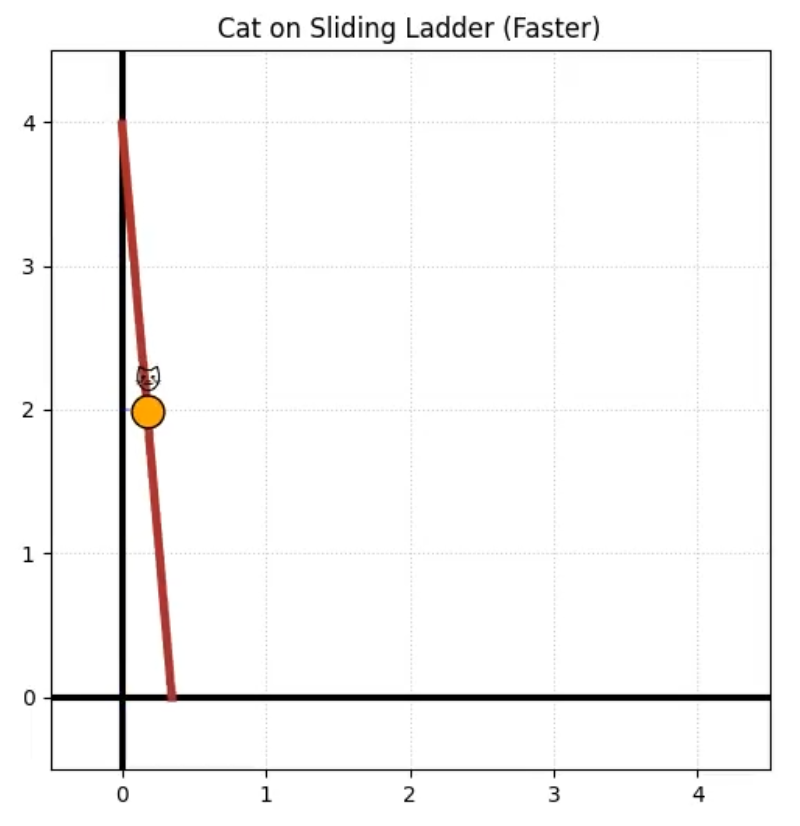
\includegraphics[width=\linewidth]{image_1.png} 
        \caption{Frame 1: Ladder starts sliding.}
    \end{subfigure}
    \hfill
    % Box 2 (Top Right)
    \begin{subfigure}[b]{0.45\textwidth}
        \centering
        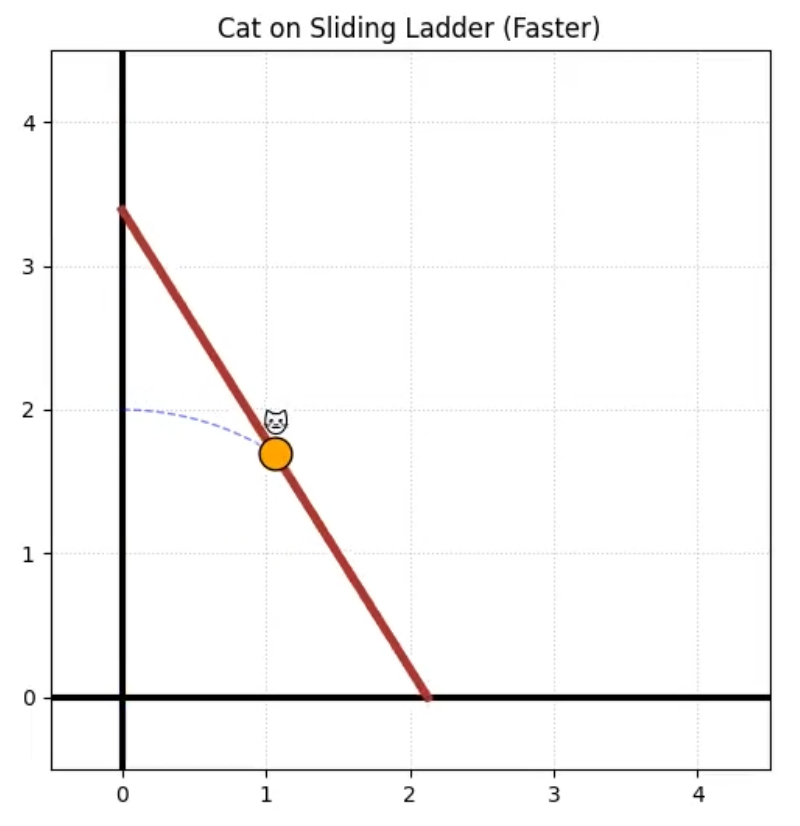
\includegraphics[width=\linewidth]{image_2.png}
        \caption{Frame 2: Cat's path begins.}
    \end{subfigure}
    
    \vspace{0.5cm} % Space between rows
    
    % Box 3 (Bottom Left)
    \begin{subfigure}[b]{0.45\textwidth}
        \centering
        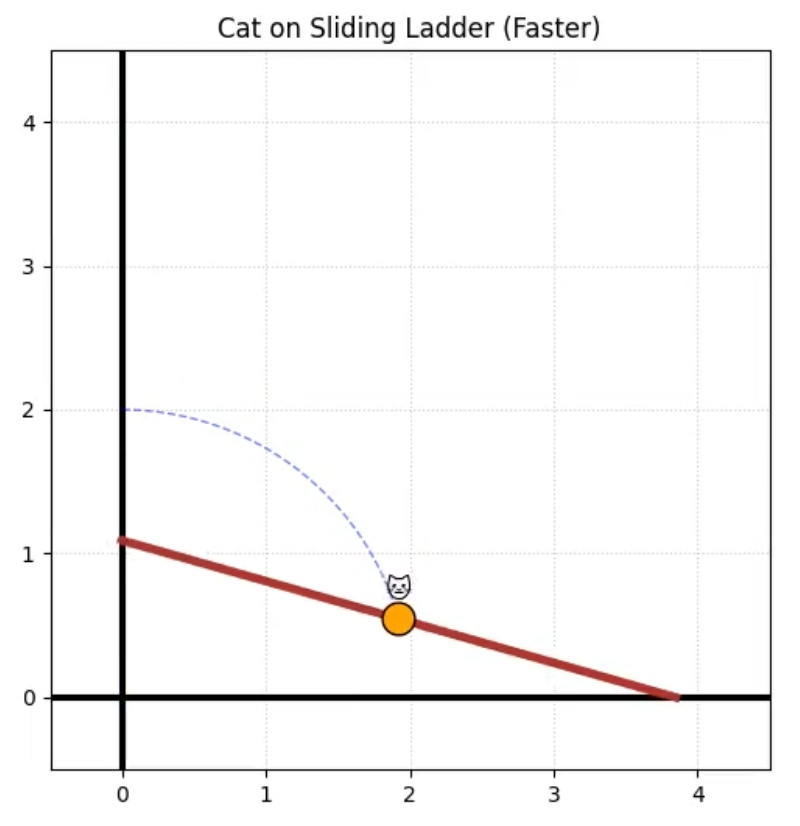
\includegraphics[width=\linewidth]{image_3.png}
        \caption{Frame 3: Circular arc becomes visible.}
    \end{subfigure}
    \hfill
    % Box 4 (Bottom Right)
    \begin{subfigure}[b]{0.45\textwidth}
        \centering
        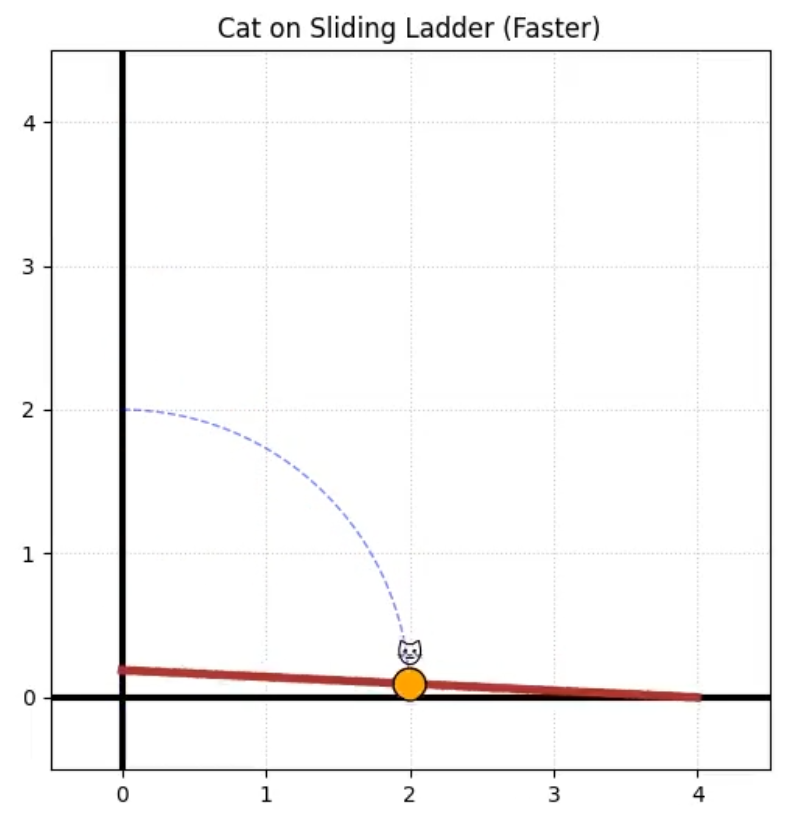
\includegraphics[width=\linewidth]{image_4.png}
        \caption{Frame 4: Ladder hits the floor.}
    \end{subfigure}
    
    \caption{The Cat on the Sliding Ladder: A visual progression over time.}
    \label{fig:sliding_ladder_grid}
\end{figure}
\vspace{0.5cm}

% ======================================================================
% GITHUB REPOSITORY LINK BOX 
% ======================================================================
\begin{mdframed}[backgroundcolor=gray!10, linecolor=black, linewidth=1pt, roundcorner=5pt]
    \centering
    \textbf{Interactive Code Available!} \\
    \vspace{0.2cm}
    You can view, run, and experiment with the full Python source code for the sliding ladder animation and other geometries in the official GitHub repository: \\
    \vspace{0.3cm}
    
    \small 
    \href{https://github.com/Shubham18024/Python-Mathematical-Animation/blob/main/2d-anim/scripts/cat_at_middle_ladder.py}{
        \color{blue}\underline{Click here to view: cat\_at\_middle\_ladder.py}
    } \\
    \vspace{0.1cm}
    \scriptsize \texttt{https://github.com/Shubham18024/Python-Mathematical-Animation/} \\
    \texttt{blob/main/2d-anim/scripts/cat\_at\_middle\_ladder.py}
\end{mdframed}
% ======================================================================

\newpage

\section{Visualizing Metric Spaces: $L_p$ Norms}

Beyond classical kinematics, the framework was utilized to visualize abstract functional spaces. The $L_p$ norm defines mathematical "distance." By rendering the unit ball ($||x||_p = 1$) for various values of $p$, we can observe the topological morphing of the space. 

As shown in the grid below, the geometry shifts from a sharp diamond ($p=1$) to a perfect Euclidean circle ($p=2$), and ultimately converges toward a square boundary ($p=\infty$).

% ======================================================================
% 4-PHOTO GRID FOR THE L_p UNIT BALLS
% ======================================================================
\vspace{0.5cm}
\begin{figure}[h!]
    \centering
    % Box 1
    \begin{subfigure}[b]{0.45\textwidth}
        \centering
        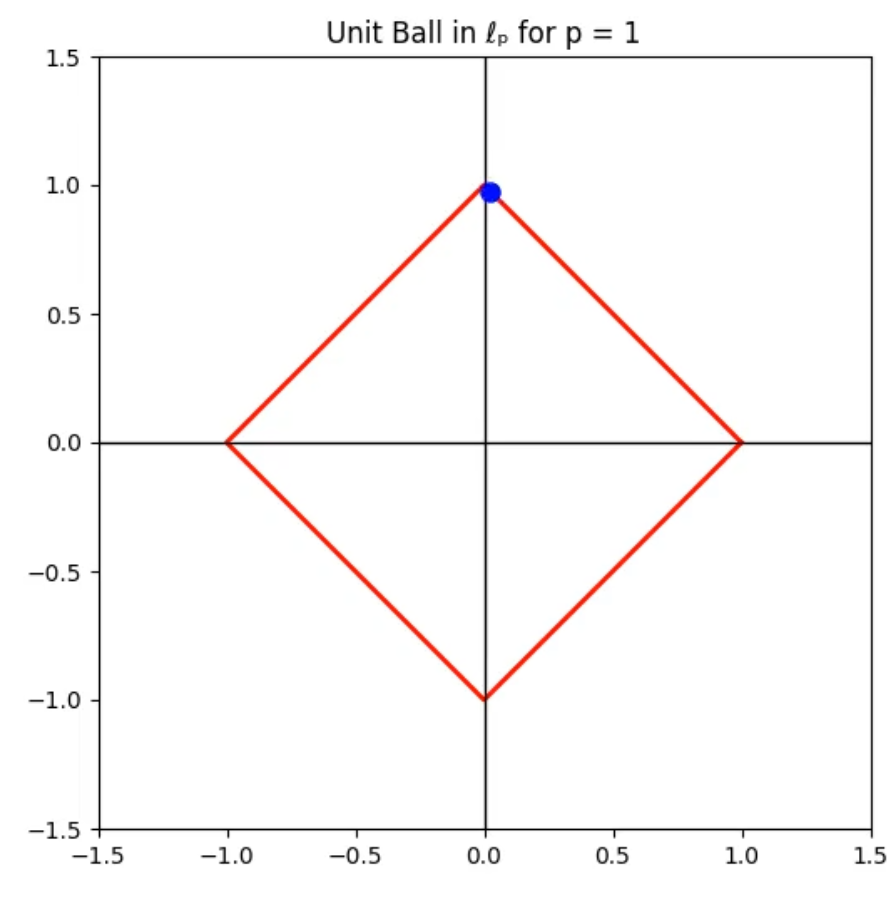
\includegraphics[width=\linewidth]{norm_p1.png} 
        \caption{$p=1$: The Diamond Shape.}
    \end{subfigure}
    \hfill
    % Box 2
    \begin{subfigure}[b]{0.45\textwidth}
        \centering
        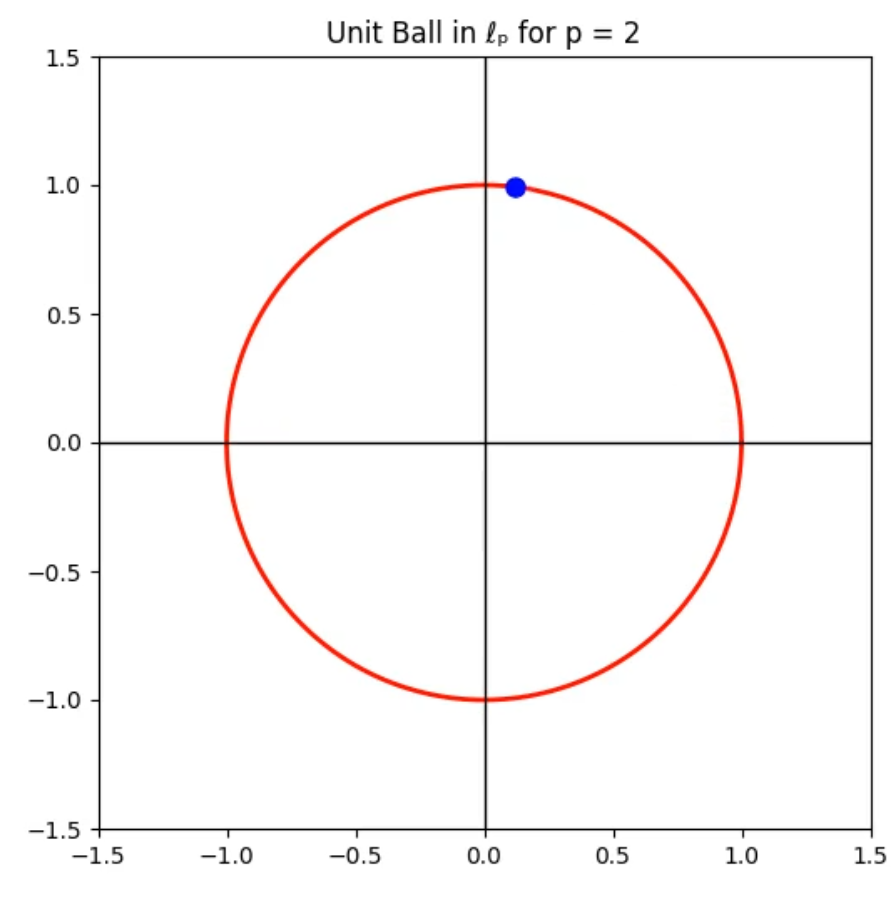
\includegraphics[width=\linewidth]{norm_p2.png}
        \caption{$p=2$: The Standard Circle.}
    \end{subfigure}
    
    \vspace{0.5cm} 
    
    % Box 3
    \begin{subfigure}[b]{0.45\textwidth}
        \centering
        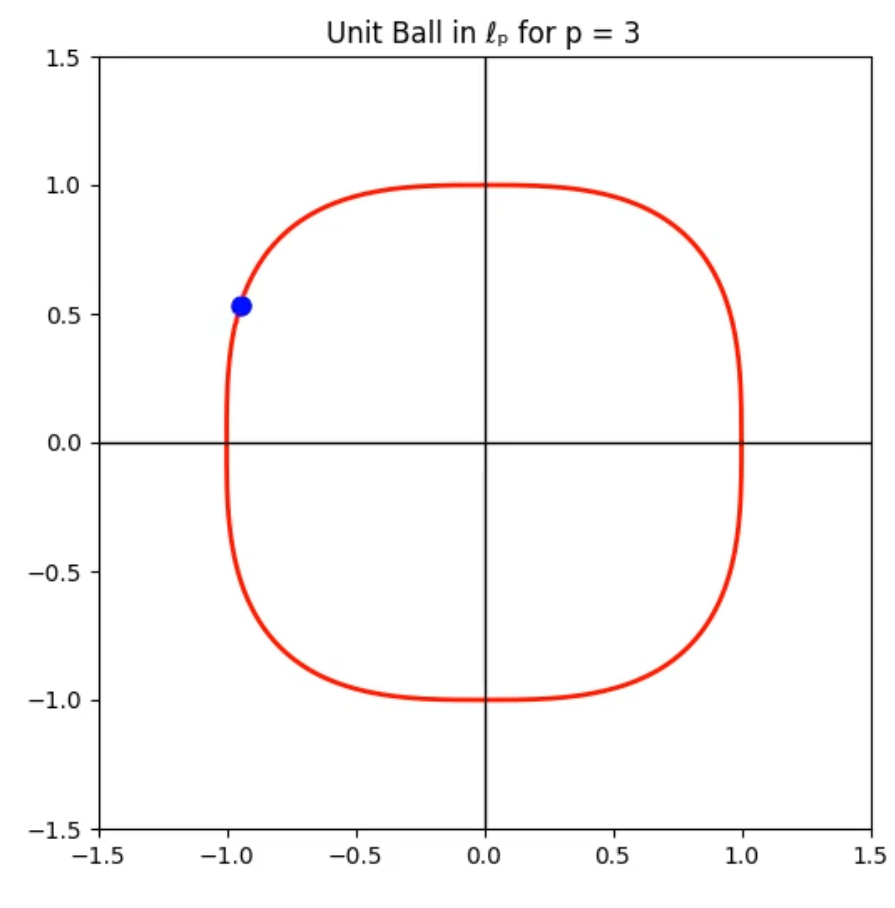
\includegraphics[width=\linewidth]{norm_p3.png}
        \caption{$p=3$: Warping towards a square.}
    \end{subfigure}
    \hfill
    % Box 4
    \begin{subfigure}[b]{0.45\textwidth}
        \centering
        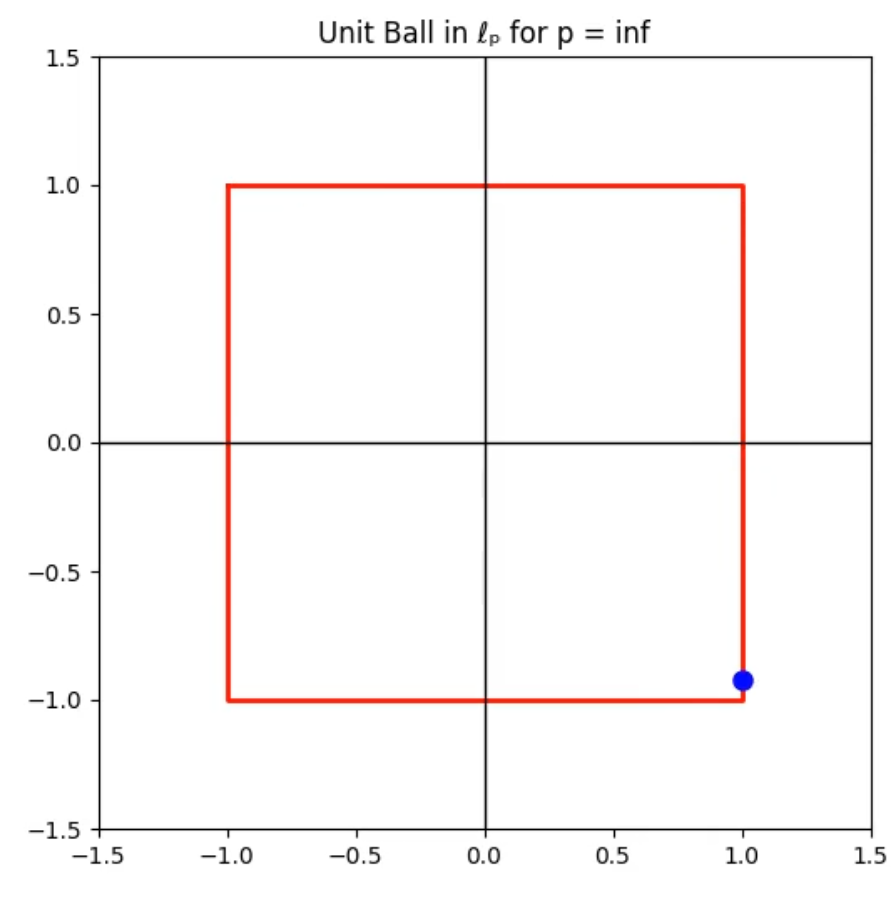
\includegraphics[width=\linewidth]{norm_pinf.png}
        \caption{$p=\infty$: The Square Boundary.}
    \end{subfigure}
    
    \caption{Visual progression of the $l_p$ unit ball as $p$ increases.}
    \label{fig:lp_norms_grid}
\end{figure}

\newpage

\section{3D Surface Geometry and Rigid Body Dynamics}

Transitioning from 2D to 3D visualization introduces significant computational complexity. The engine must evaluate bivariate parametric grids and apply $SO(3)$ rotation matrices to every vertex simultaneously. The following sections showcase the successful rendering and animation of various 3D mathematical systems.

\subsection{Fundamental Rigid Bodies}
The first test of the 3D engine was to ensure that basic geometric primitives could be rotated without distorting their volume or structural integrity.

% --- GRID 1: BASIC 3D SHAPES (2x2) ---
\vspace{0.4cm}
\begin{figure}[htbp]
    \centering
    \begin{subfigure}[b]{0.45\textwidth}
        \centering
        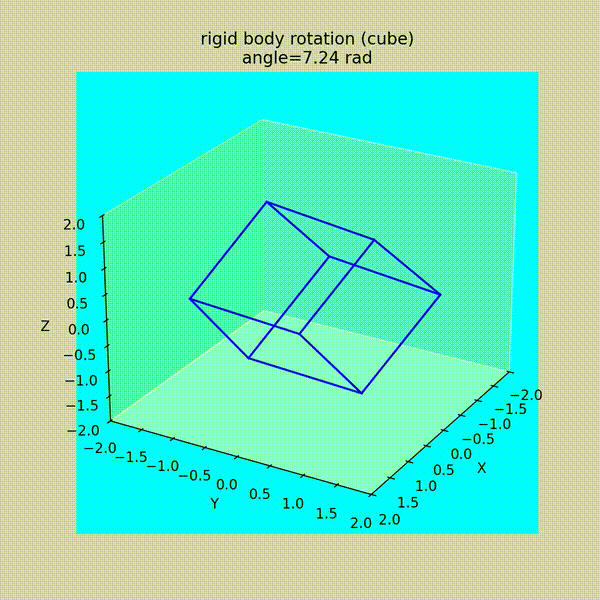
\includegraphics[width=\linewidth]{cube_rotation.png} 
        \caption{Standard rigid cube rotation.}
    \end{subfigure}
    \hfill
    \begin{subfigure}[b]{0.45\textwidth}
        \centering
        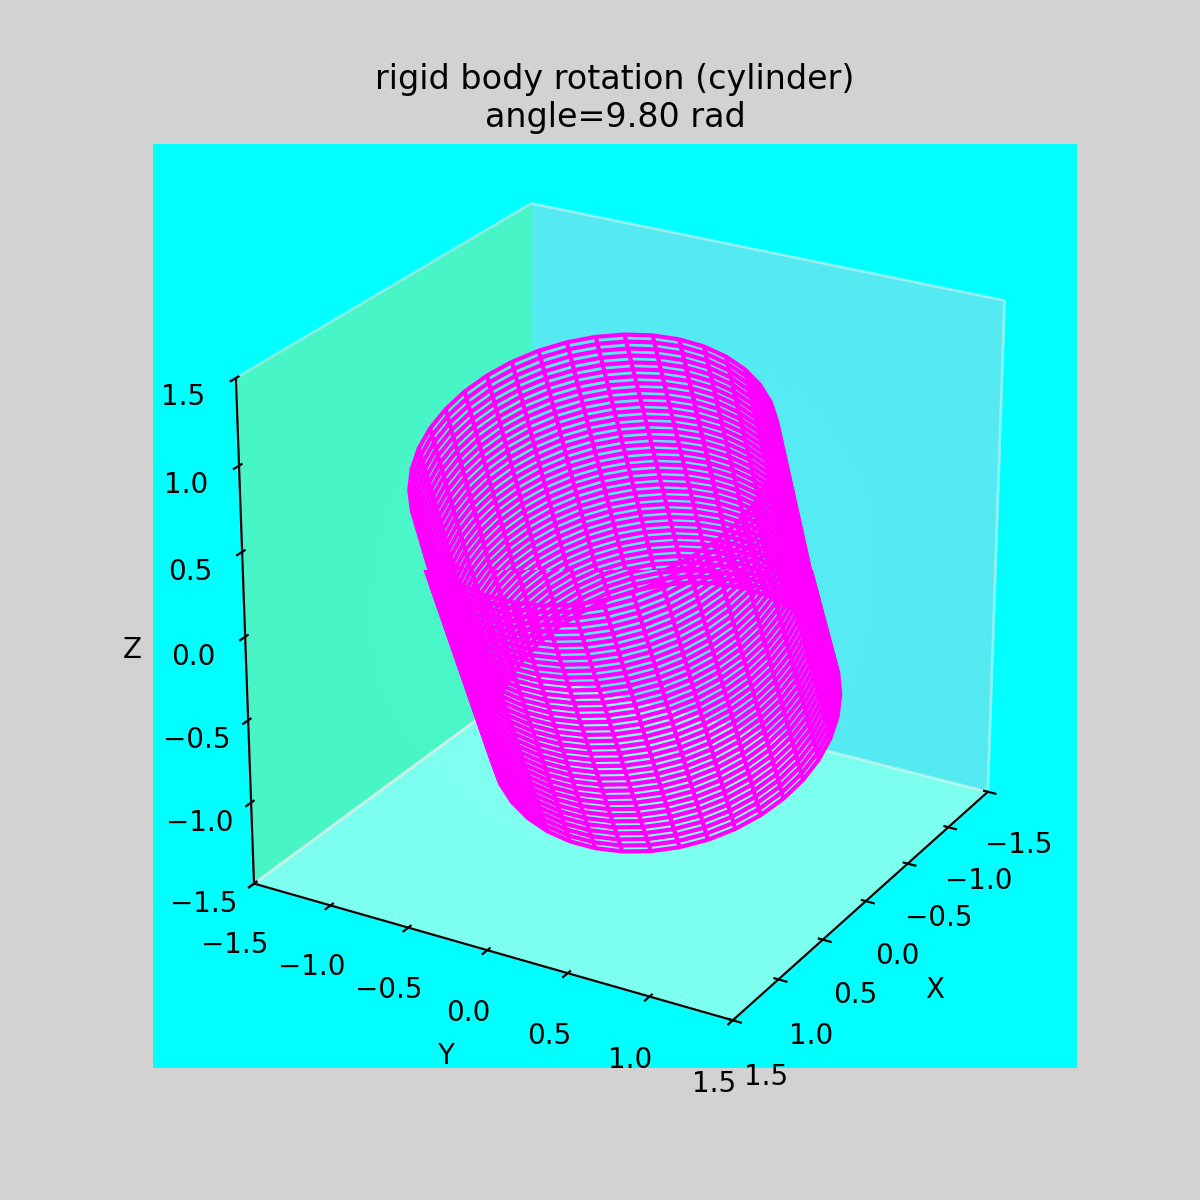
\includegraphics[width=\linewidth]{cylinder_rotation.png}
        \caption{Parametric cylinder rotation.}
    \end{subfigure}
    
    \vspace{0.5cm} 
    
    \begin{subfigure}[b]{0.45\textwidth}
        \centering
        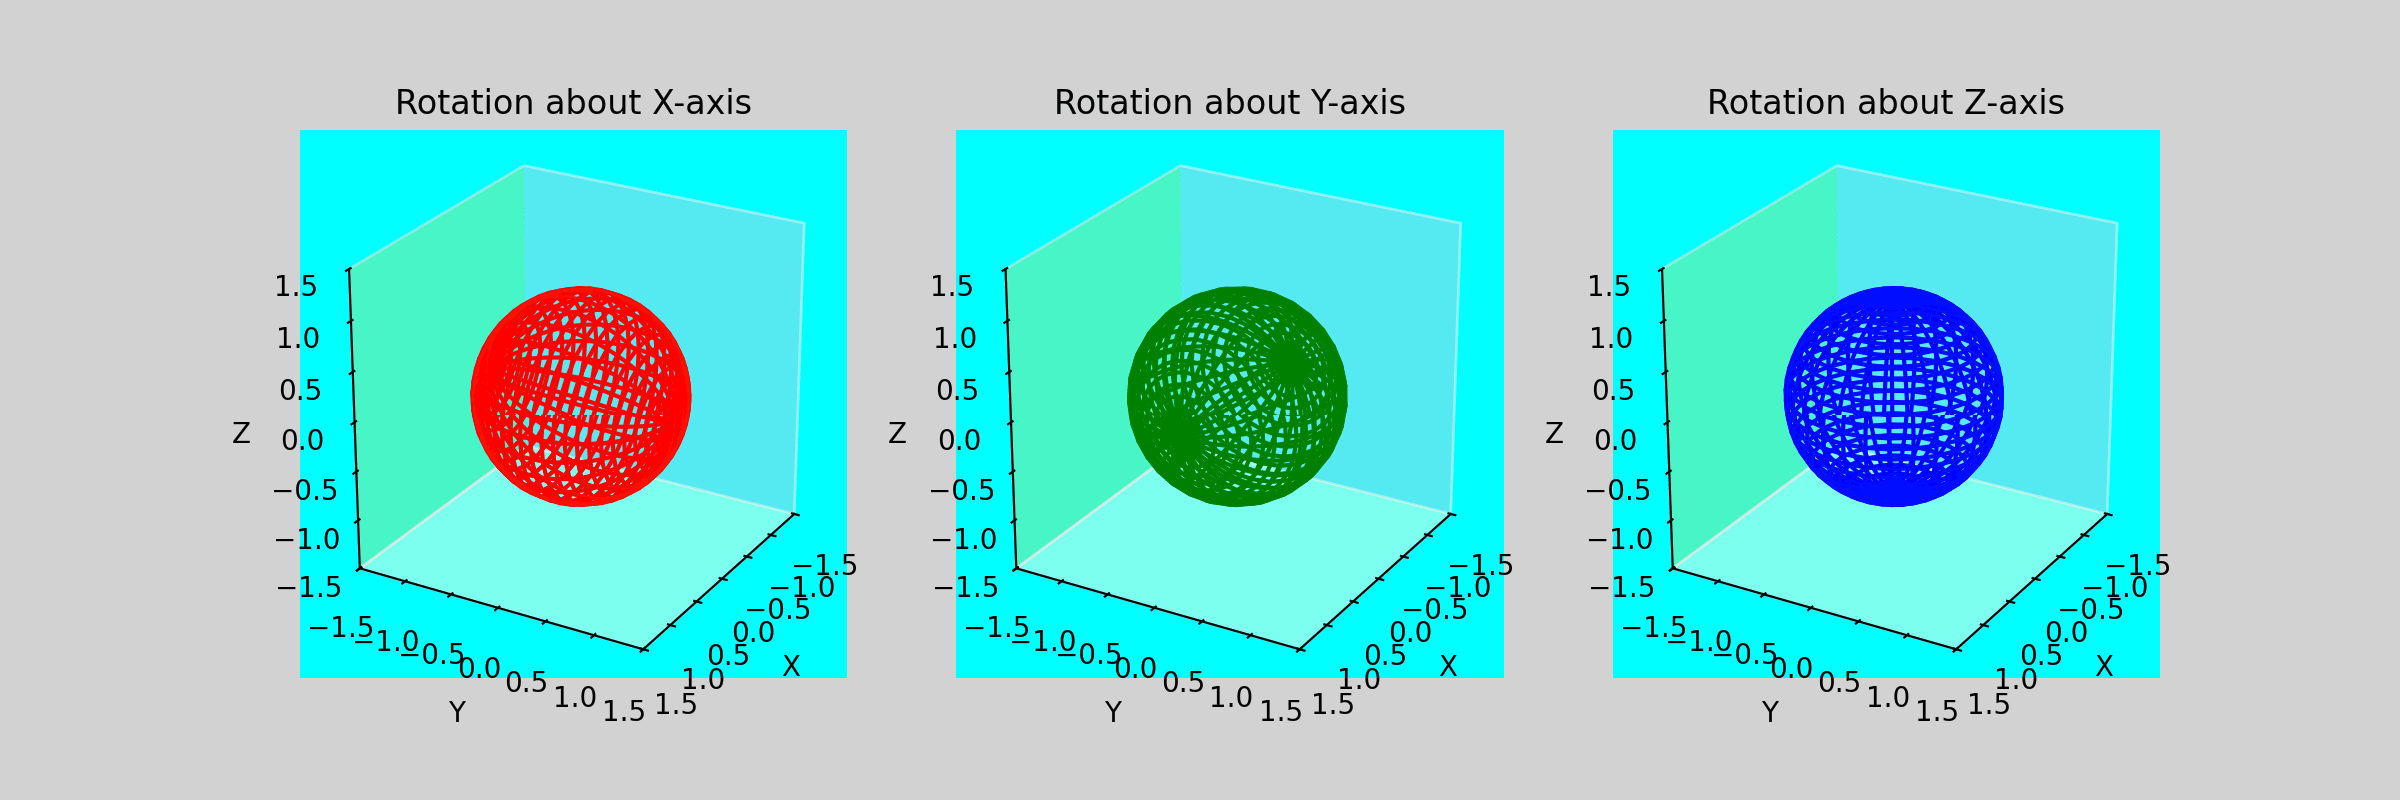
\includegraphics[width=\linewidth]{sphere_multiple_axes_rotation.png}
        \caption{Spheres rotating on multiple axes.}
    \end{subfigure}
    \hfill
    \begin{subfigure}[b]{0.45\textwidth}
        \centering
        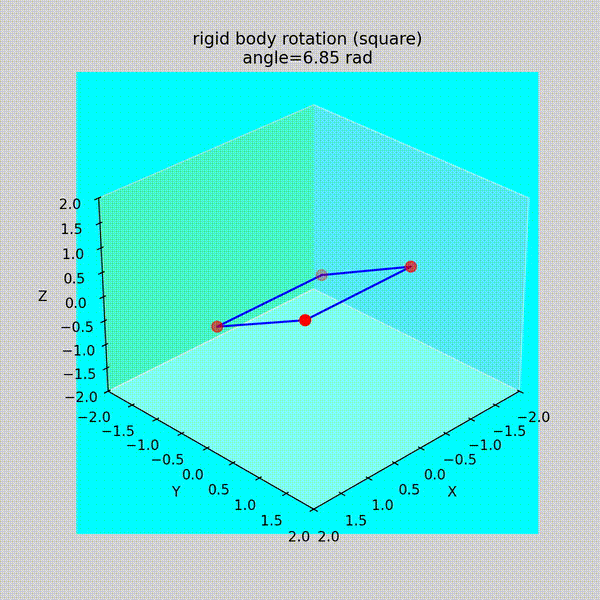
\includegraphics[width=\linewidth]{square_rotation.png}
        \caption{2D square rotating in 3D space.}
    \end{subfigure}
    
    \caption{Fundamental geometric rigid body rotations.}
    \label{fig:3d_basic}
\end{figure}

\subsection{Complex and Minimal Surfaces}
Beyond basic shapes, the engine was used to visualize advanced differential geometry. This includes minimal surfaces (surfaces that locally minimize their area, like soap films) and topological immersions (like Boy's Surface).

% --- GRID 2: ADVANCED SURFACES (2x2) ---
\vspace{0.4cm}
\begin{figure}[htbp]
    \centering
    \begin{subfigure}[b]{0.45\textwidth}
        \centering
        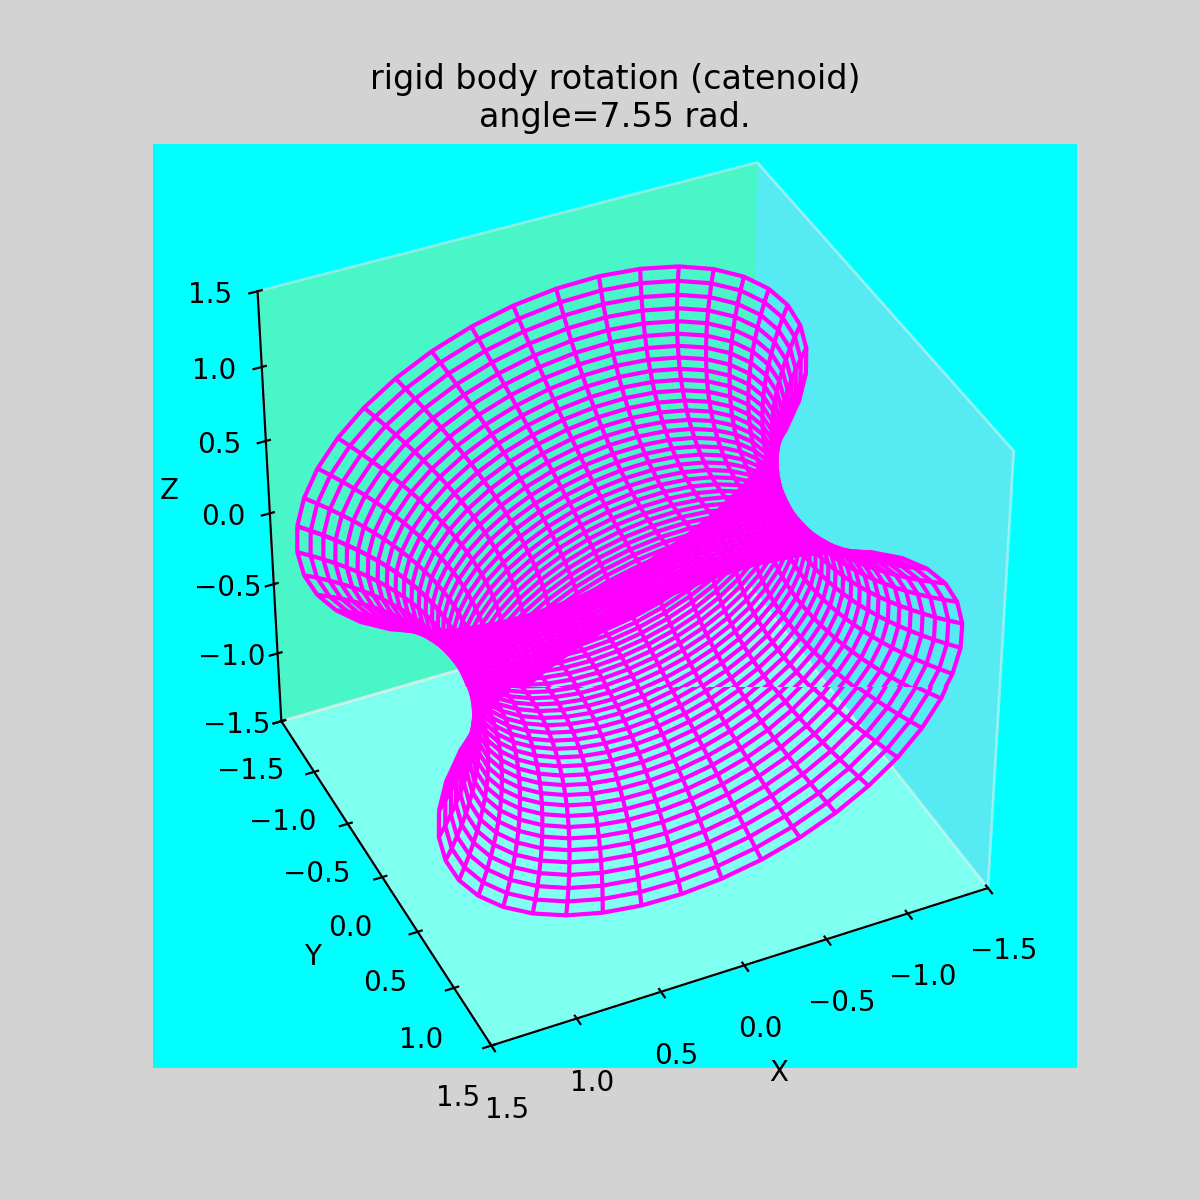
\includegraphics[width=\linewidth]{catenoid_rotation.png} 
        \caption{The Catenoid (Minimal Surface).}
    \end{subfigure}
    \hfill
    \begin{subfigure}[b]{0.45\textwidth}
        \centering
        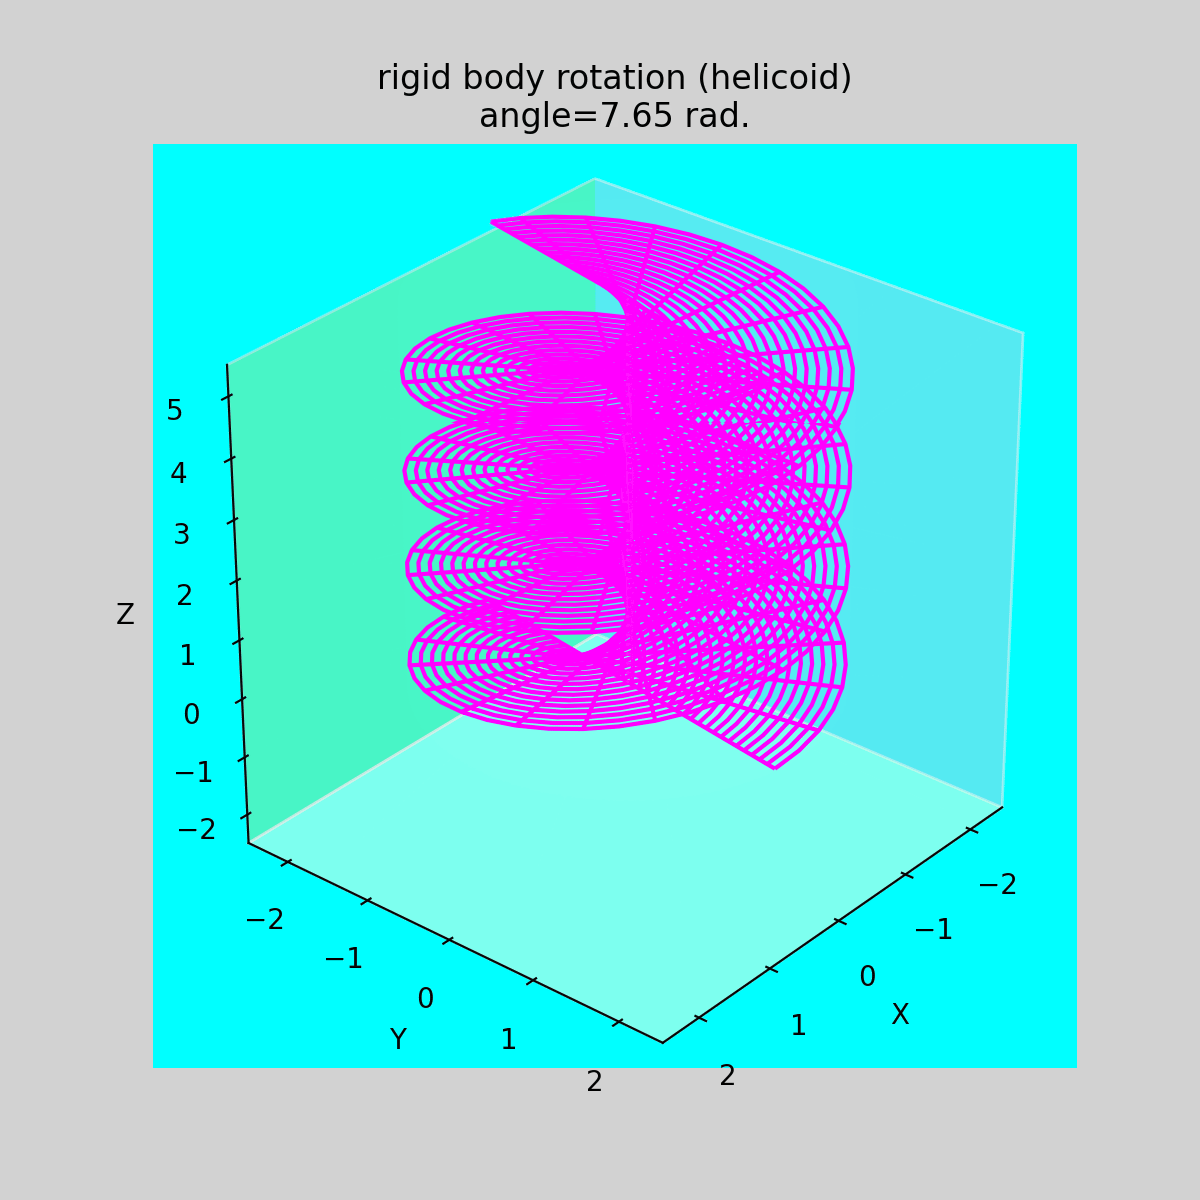
\includegraphics[width=\linewidth]{helicoid_rotation.png}
        \caption{The Helicoid (Ruled Minimal Surface).}
    \end{subfigure}
    
    \vspace{0.5cm} 
    
    \begin{subfigure}[b]{0.45\textwidth}
        \centering
        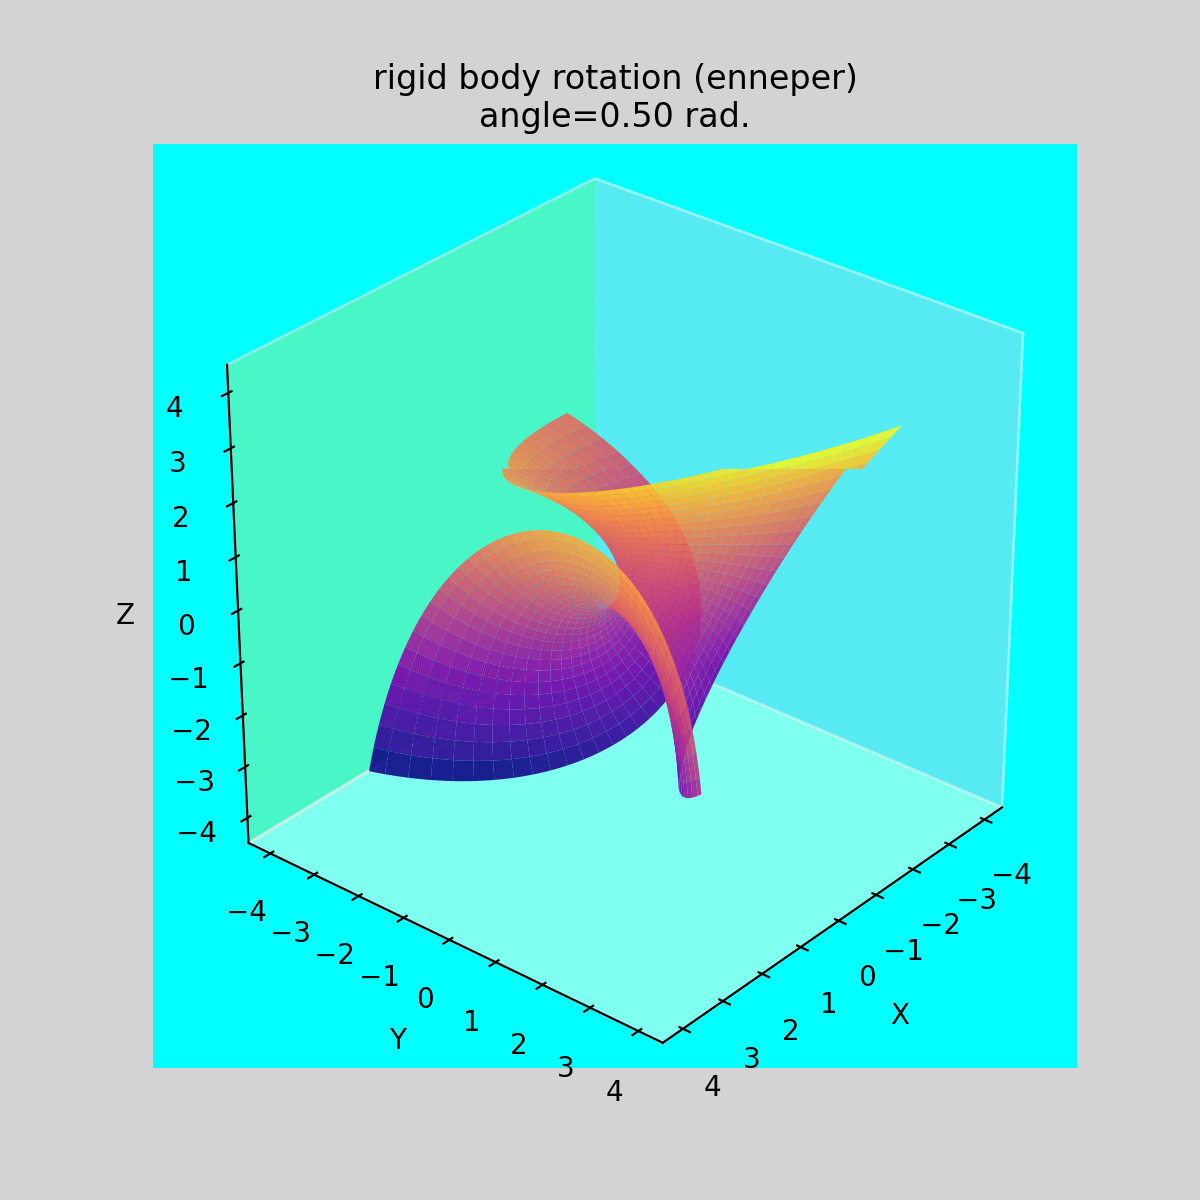
\includegraphics[width=\linewidth]{enneper_rotation.png}
        \caption{Enneper's Surface (Self-intersecting).}
    \end{subfigure}
    \hfill
    \begin{subfigure}[b]{0.45\textwidth}
        \centering
        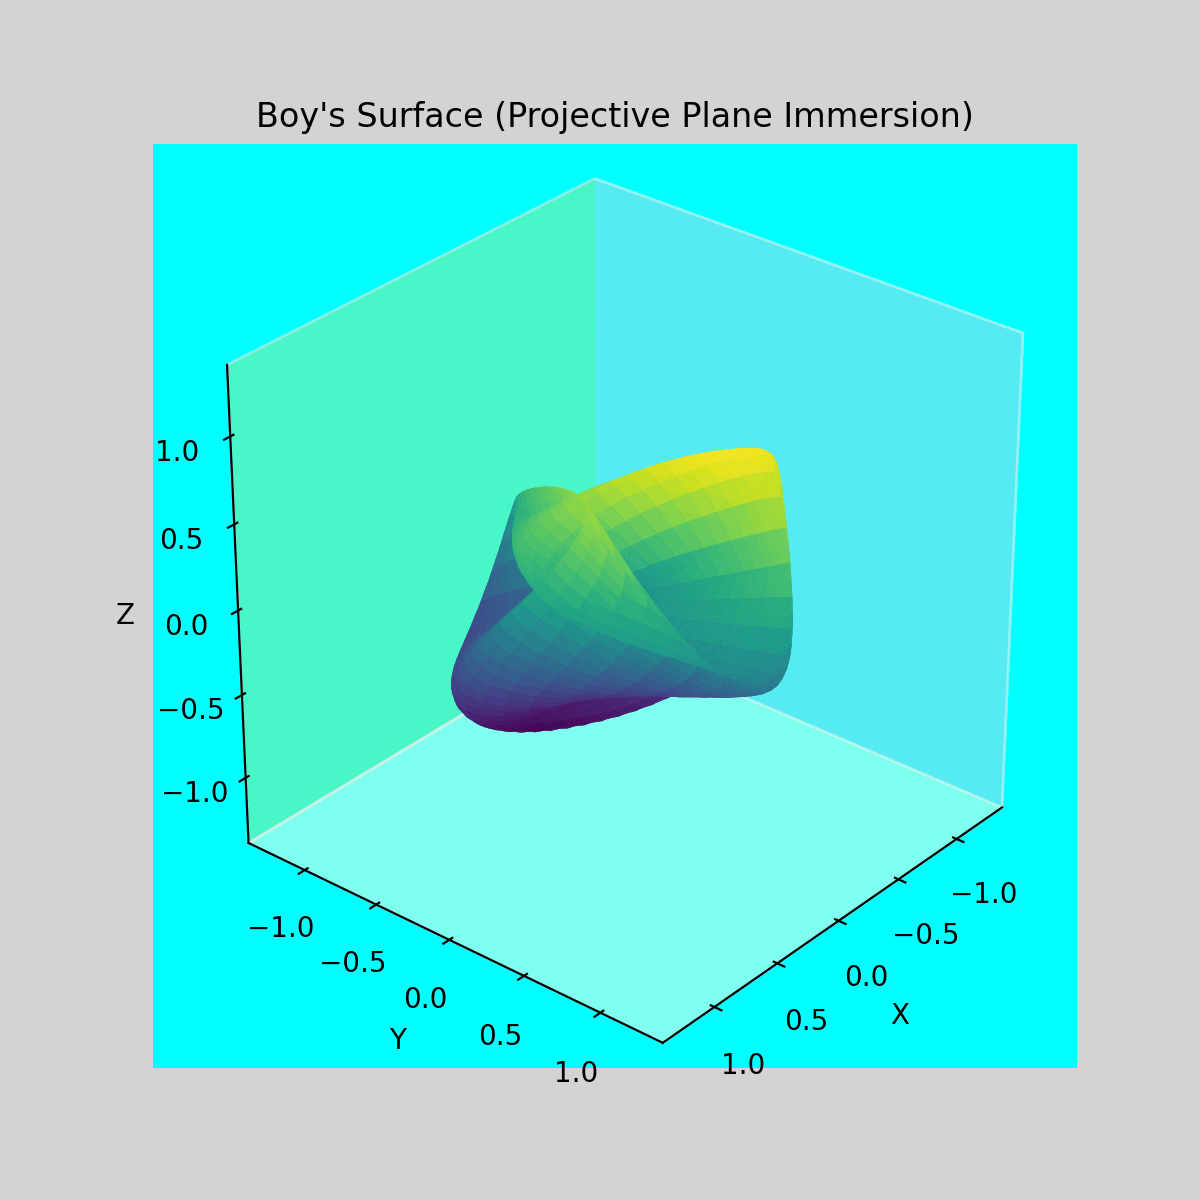
\includegraphics[width=\linewidth]{boys_surface_rotation.png}
        \caption{Boy's Surface ($RP^2$ immersion).}
    \end{subfigure}
    
    \caption{Visualization of advanced differential geometry.}
    \label{fig:3d_advanced}
\end{figure}
\vspace{0.4cm}

\subsection{Dynamic Systems and Transformations}
The most advanced capability of the animation engine is handling multiple moving objects, topological transformations, and combined translation-rotation kinematics. 

% --- GRID 3: SYSTEMS & TRANSFORMS (2x2) ---
\begin{figure}[htbp]
    \centering
    \begin{subfigure}[b]{0.45\textwidth}
        \centering
        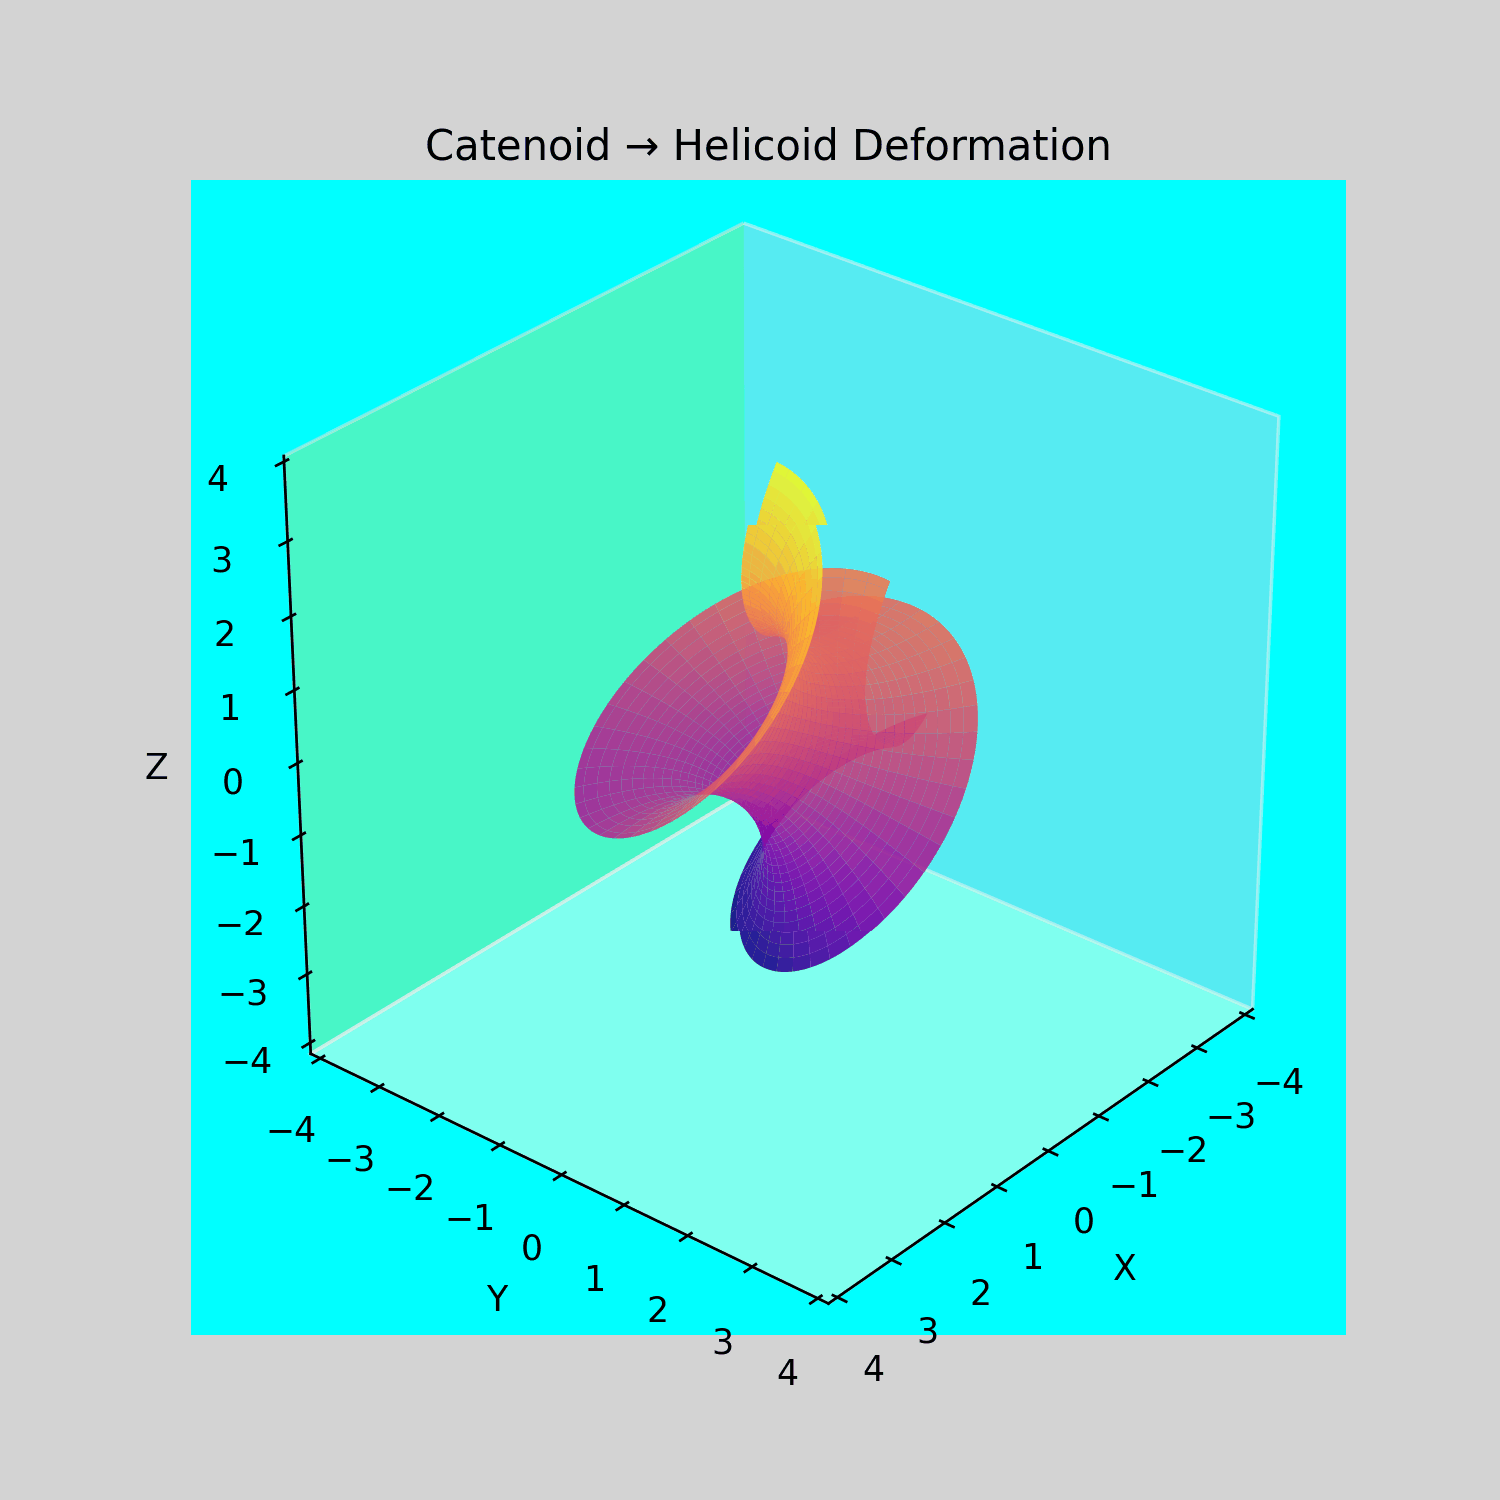
\includegraphics[width=\linewidth]{catenoid_to_helicoid_transformation.png} 
        \caption{Continuous isometric deformation.}
    \end{subfigure}
    \hfill
    \begin{subfigure}[b]{0.45\textwidth}
        \centering
        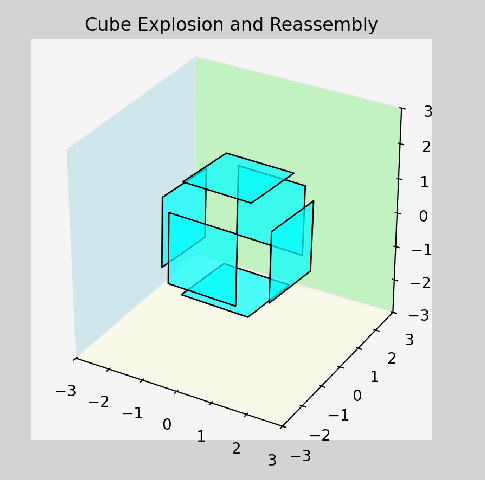
\includegraphics[width=\linewidth]{cube_explode.png}
        \caption{Cube face explosion/reassembly.}
    \end{subfigure}
    
    \vspace{0.5cm} 
    
    \begin{subfigure}[b]{0.45\textwidth}
        \centering
        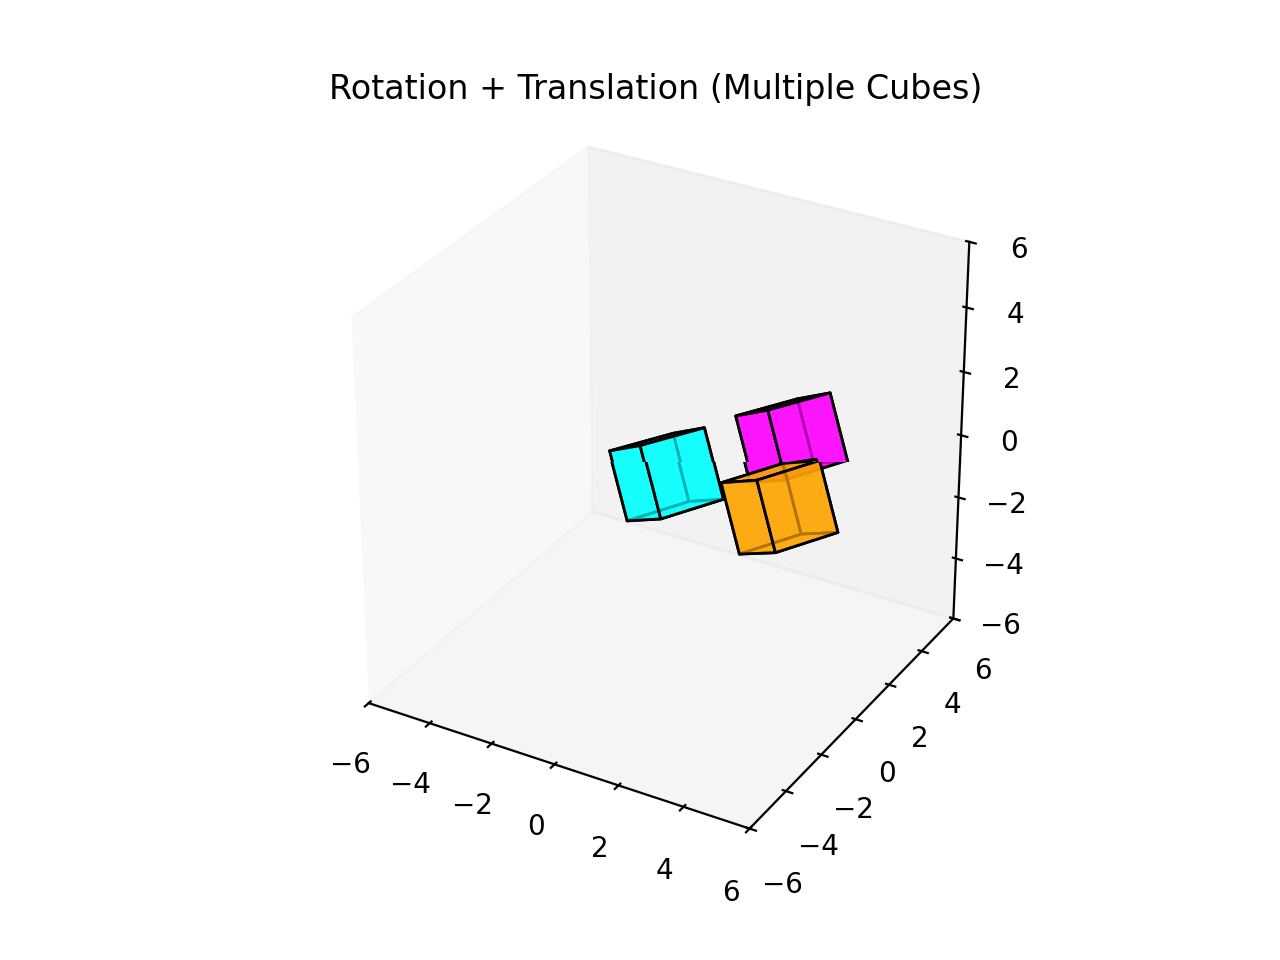
\includegraphics[width=\linewidth]{Multiple_Cubes_translation_rotation.png}
        \caption{Multi-cube translation and rotation.}
    \end{subfigure}
    \hfill
    \begin{subfigure}[b]{0.45\textwidth}
        \centering
        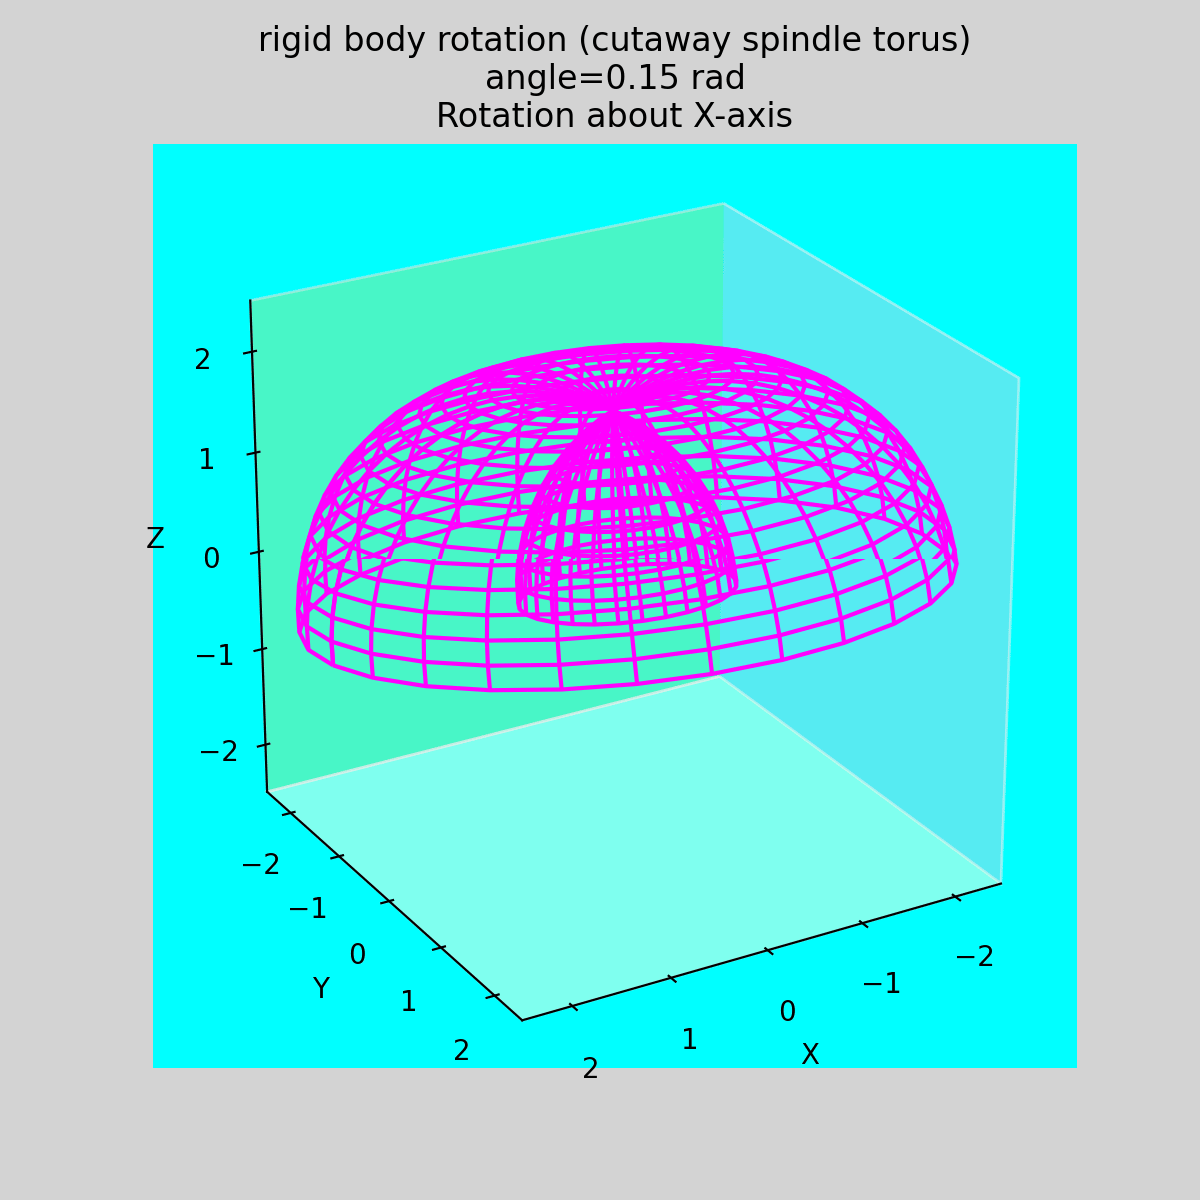
\includegraphics[width=\linewidth]{cutaway_spindle_torus_rotation.png}
        \caption{Cutaway view of a Spindle Torus.}
    \end{subfigure}
    
    \caption{Dynamic multi-body systems and topological transformations.}
    \label{fig:3d_systems}
\end{figure}

% --- SINGLE FIGURE: HUMAN MOTION ---
\vspace{0.4cm}
\begin{figure}[htbp]
    \centering
    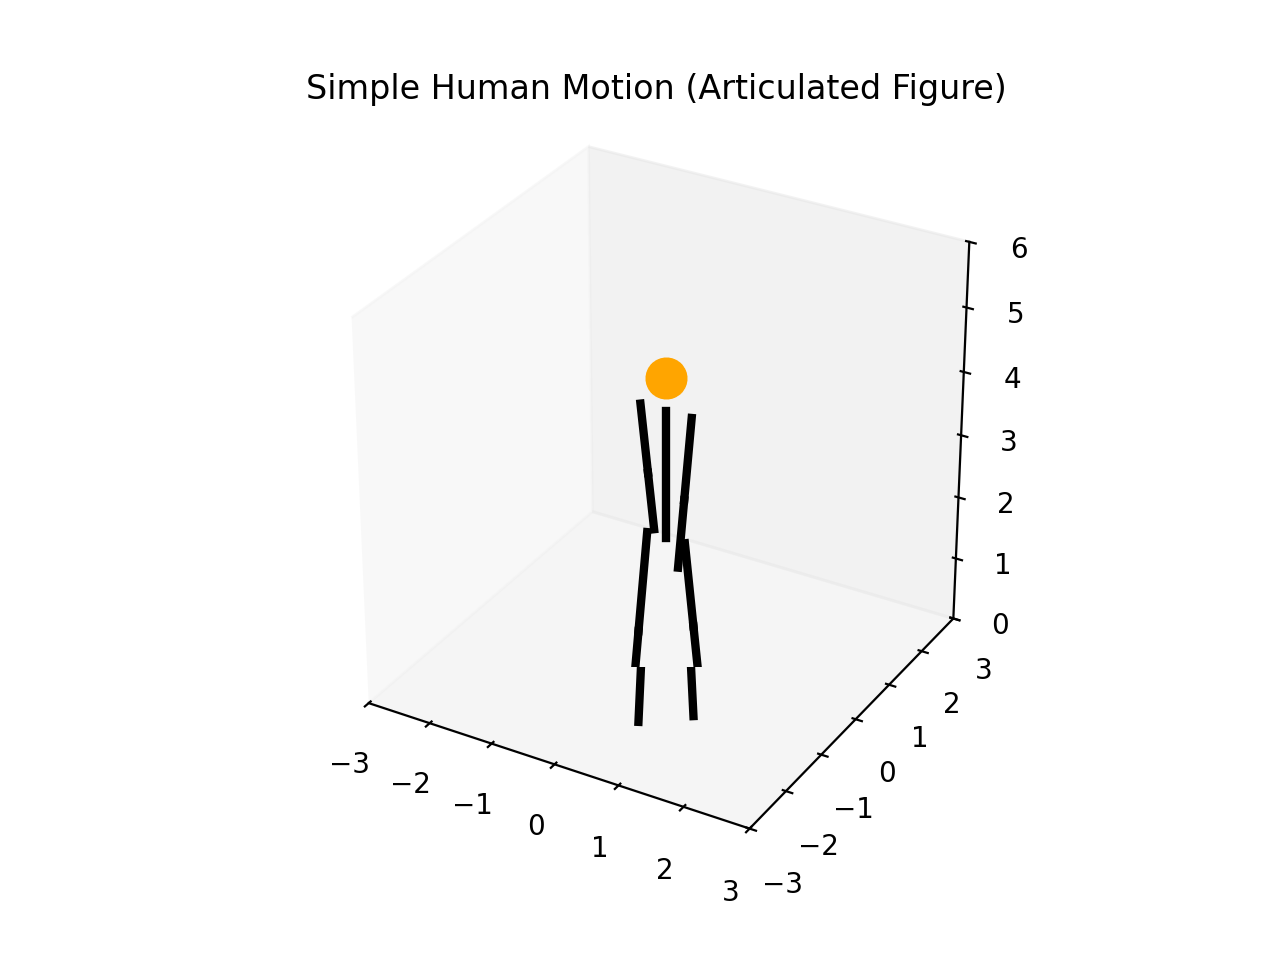
\includegraphics[width=0.65\textwidth]{Human_Motion.png}
    \caption{Combining multiple geometric arrays to simulate human kinematic motion.}
    \label{fig:human_motion}
\end{figure}


\chapter{Challenges Faced}

Developing this project and especially a custom mathematical engine from the starting that suits your requirement isn't easy. I always tried to bridge the gap between pure abstract geometrical concepts and discrete computation, but throughout this several technical, mathematical, environmental and system barriers were faced and then also resolved in the organized way.

\section{Rendering and Performance Issues}
The primary graphical backend for this project is \texttt{Matplotlib}. While it is exceptional for static data visualization, but pushing it to the render dynamic 3D animations introduced immediate performance bottlenecks:

\begin{itemize}
    \item \textbf{CPU-Bound Processing:} Unlike modern graphics engines that utilize the GPU, \texttt{Matplotlib} calculates all rendering on the CPU. When animating complex topologies like the Helicoid with dense parametric meshes, the frame rate dropped significantly, requiring careful optimization of the \texttt{np.linspace} resolution.\cite{matplotlib_docs}
    \item \textbf{Depth Sorting (Z-buffering) Artifacts:} \texttt{Matplotlib's} 3D axis does not possess a true 3D rendering engine. It relies on a 2D projection using a basic \textbf{"painter's algorithm."} \cite{matplotlib_docs} This occasionally caused visual glitches where background polygons were incorrectly drawn on top of foreground polygons.
    \item \textbf{Memory Leaks in the Animation Loop:} Initially, continuously redrawing objects in the \texttt{update()} function caused the RAM usage to spike until the program crashed. This was solved by implementing \texttt{ax.clear()} to flush the geometry from memory on every frame before drawing the new coordinates.
\end{itemize}

\section{Mathematical Conversion and Scaling}
Translating pure mathematics into a visual medium required resolving several geometric scaling issues:

\begin{itemize}
    \item \textbf{Aspect Ratio Distortion:} By default, Python plotting libraries auto-scale axes to fit data. When rotating a 3D sphere, this auto-scaling caused the sphere to stretch into an ellipsoid depending on the viewing angle. Hardcoding \texttt{ax.set\_box\_aspect([1,1,1])} and manually enforcing isometric axis limits was necessary to preserve rigid body dimensions.
    \item \textbf{Boy's Surface Plotting:} Plotting of Minimal surfaces isn't easy especially \texttt{Boy's Surface}, we use its approximate parametrized equation to plot that surface.
    \cite{boys_surface_wiki}
    \item \textbf{Continuous to Discrete Mapping:} Mathematical curves extend to infinity, but computers can only draw discrete points. Finding the exact mathematical step-size (e.g., $\Delta\theta = 0.05$) was a constant balancing act between making curves look perfectly smooth and keeping the rendering speed high.
\end{itemize}

\section{Environment and Dependency Bugs}
Managing a Python environment for graphical rendering across different operating systems introduced "dependency hell":

\begin{itemize}
    \item \textbf{Library Version Conflicts:} Early in development, mismatched versions of \texttt{NumPy} and \texttt{Matplotlib} caused matrix multiplication functions (\texttt{@} operator) to fail. This is why the project migrated to \textbf{\texttt{uv}}, which completely eliminated these crashes by strictly locking dependency versions in the \texttt{pyproject.toml} file.\cite{uv_docs}
    \item \textbf{Video Export Failures (\texttt{FFmpeg}):} While displaying the animation on the screen worked perfectly, saving the animations as \texttt{.mp4} or \texttt{.gif} files required an external binary called \texttt{FFmpeg}. Debugging path variable errors and codec issues within the Linux/Ubuntu environment was a major challenge before the video export pipeline was finally stabilized.\cite{matplotlib_docs}
\end{itemize}

\vspace{0.6cm}
Overcoming these challenges required a deep understanding of both linear algebra and programming skills, ultimately resulting in the highly stable and reproducible animation framework presented in this project work.

%===============================================
%Chapter 11
%===============================================
\chapter{Conclusion and Future Scope}

\section{Summary of Achievements}
This project successfully connected pure mathematical theory with computational visualization. By using principles from coordinate geometry, linear algebra, and differential geometry, we developed a strong, open-source Python animation engine. 

The project turned static math concepts—like the sliding ladder constraint, $SO(3)$ rotation matrices, and $L_p$ norm spaces—into dynamic, time-dependent computational systems. Additionally, the successful rendering of complex topological shapes, such as Boy’s Surface and the Catenoid-Helicoid transformation, proves that programmatic animation is a valuable tool for modern math education.

\section{Current Limitations}
While the project met its main visualization goals, it is important to recognize the computational limitations of the current setup:
\begin{itemize}
    \item \textbf{CPU-Bound Rendering:} \texttt{Matplotlib} handles 3D rendering on the CPU instead of the GPU. With highly complex shapes that have thousands of vertices, the frame rate drops, making real-time interaction slow.
    \item \textbf{Lack of Real-Time Interactivity:} Right now, animations are pre-calculated and shown as loops or exported videos. Users cannot easily drag a vertex or change a setting through a graphical slider during an animation without editing the source code.
    \item \textbf{Pseudo-3D Projection:} \texttt{Matplotlib}'s 3D axis does not support true depth-buffering (Z-buffering) or advanced lighting methods, which sometimes causes visual issues where background faces appear on top of foreground faces.
\end{itemize}

\section{Future Scope}
To build on the foundation laid by this project, future development can explore several technical paths:

\begin{enumerate}
    \item \textbf{Migration to High-Performance Graphics Engines:} 
    To address the CPU limitations, future versions of this code could shift the mathematical logic to GPU-accelerated frameworks. Using libraries like \texttt{Manim} (designed for math animation) or \texttt{Three.js} (for web browsers) would enable rendering complex lighting and true Z-buffering at 60 frames per second.
    
    \item \textbf{Graphical User Interface (GUI) Development:}
    Creating a dedicated application frontend with \texttt{PyQt} or \texttt{CustomTkinter} would let students enter their own parametric equations, adjust slider values for radius or time, and see the geometry respond in real-time without needing to deal with the raw Python scripts.
    
    \item \textbf{Integration of Physics Engines:}
    Currently, the animations rely solely on geometric rules and time parameters. Future work could add rigid-body physics engines (like \texttt{SciPy}'s numerical ODE solvers) to introduce mass, gravity, inertia, and collision detection into the mathematical models.
\end{enumerate}

\vspace{1cm}
\begin{center}
    \textit{"Nature’s patterns are the most beautiful,\\ but they are all governed
by the same mathematical laws. In computer animation,\\ we don’t just
draw; we simulate the laws of the universe."} \\
    --- ED Catmull (Founder of Pixar Studios)
\end{center}

% ==============================================================================
% AFTER CHAPTERS: BACKMATTER
% ==============================================================================

% ------------------------------------------------------------------------------
% REFERENCES
% ------------------------------------------------------------------------------
% USER INSTRUCTION: Update these references with your actual citations.
% ------------------------------------------------------------------------------
% REFERENCES
% ------------------------------------------------------------------------------
\begin{thebibliography}{99}
\addcontentsline{toc}{chapter}{References}

\bibitem{waxman2023}
Waxman, J. (2023). \textit{Cognitive Theory of Multimedia Learning} [Monograph]. Center for Health Decision Science, Harvard T.H. Chan School of Public Health. Available at: \url{https://media.repository.chds.hsph.harvard.edu/static/filer_public/ca/62/ca625803-3d73-4855-b3e1-765870ce3772/2023_jwaxman_monograph_cogtheory_multimed.pdf}

\bibitem{python_docs}
Python Software Foundation. (2024). \textit{Python Language Reference, version 3.x}. Available at: \url{https://docs.python.org/3/}

\bibitem{matplotlib_docs}
Matplotlib Developers. (2024). \textit{Matplotlib Animation Guide}. Available at: \url{https://matplotlib.org/stable/api/animation_api.html}

\bibitem{numpy_docs}
NumPy Developers. (2024). \textit{NumPy Official Documentation}. Available at: \url{https://numpy.org/doc/stable/}

\bibitem{uv_docs}
Astral. (2024). \textit{uv: An extremely fast Python package installer and resolver, written in Rust}. Astral. Available at: \url{https://github.com/astral-sh/uv}

\bibitem{boys_surface_wiki}
Wikipedia contributors. (2026). \textit{Boy's surface}. Wikipedia, The Free Encyclopedia. Available at: \url{https://en.wikipedia.org/wiki/Boy's_surface}

\bibitem{loney1895}
Loney, S. L. (1895). \textit{The Elements of Coordinate Geometry}. London: Macmillan and Co.

\bibitem{kreyszig1989}
Kreyszig, E. (1989). \textit{Introductory Functional Analysis with Applications}. John Wiley \& Sons. Wiley-India Student Edition.

\bibitem{friedberg2019}
Friedberg, S. H., Insel, A. J., \& Spence, L. E. (2019). \textit{Linear Algebra} (5th ed.). Pearson Education India.

\bibitem{kobayashi2019}
Kobayashi, S. (2019). \textit{Differential Geometry of Curves and Surfaces}. Springer Nature Singapore. Corrected publication 2021. \url{https://doi.org/10.1007/978-981-15-1739-6}

\end{thebibliography}



\clearpage

% ------------------------------------------------------------------------------
% APPENDICES
% ------------------------------------------------------------------------------
\appendix

% =========================================================
% APPENDIX A
% =========================================================
\chapter{Open-Source Code \& GitHub Repository}
\label{app:github}

The complete Python source code, including all Jupyter Notebooks, python scripts, and rendered assets discussed in this project, has been made fully open-source. 

\vspace{0.5cm}

% ======================================================================
% GITHUB REPOSITORY LINK BOX 
% ======================================================================
\begin{mdframed}[backgroundcolor=gray!10, linecolor=black, linewidth=1pt, roundcorner=5pt]
    \centering
    \vspace{0.2cm}
    \textbf{\Large Official GitHub Repository} \\
    \vspace{0.3cm}
    
    \href{https://github.com/Shubham18024/Python-Mathematical-Animation}{
        \color{blue}\underline{\texttt{https://github.com/Shubham18024/Python-Mathematical-Animation}}
    } \\
    
    \vspace{0.4cm}
    \textit{Readers are highly encouraged to clone the repository, run the interactive notebooks, \\ and collaborate or contribute to future mathematical animations.}
    \vspace{0.2cm}
\end{mdframed}

\vspace{0.8cm}

% ======================================================================
% BIG GITHUB SCREENSHOT
% ======================================================================
\begin{figure}[htbp]
    \centering
    % The framebox adds a highly professional thin black border around the screenshot
    \setlength{\fboxsep}{0pt}
    \fbox{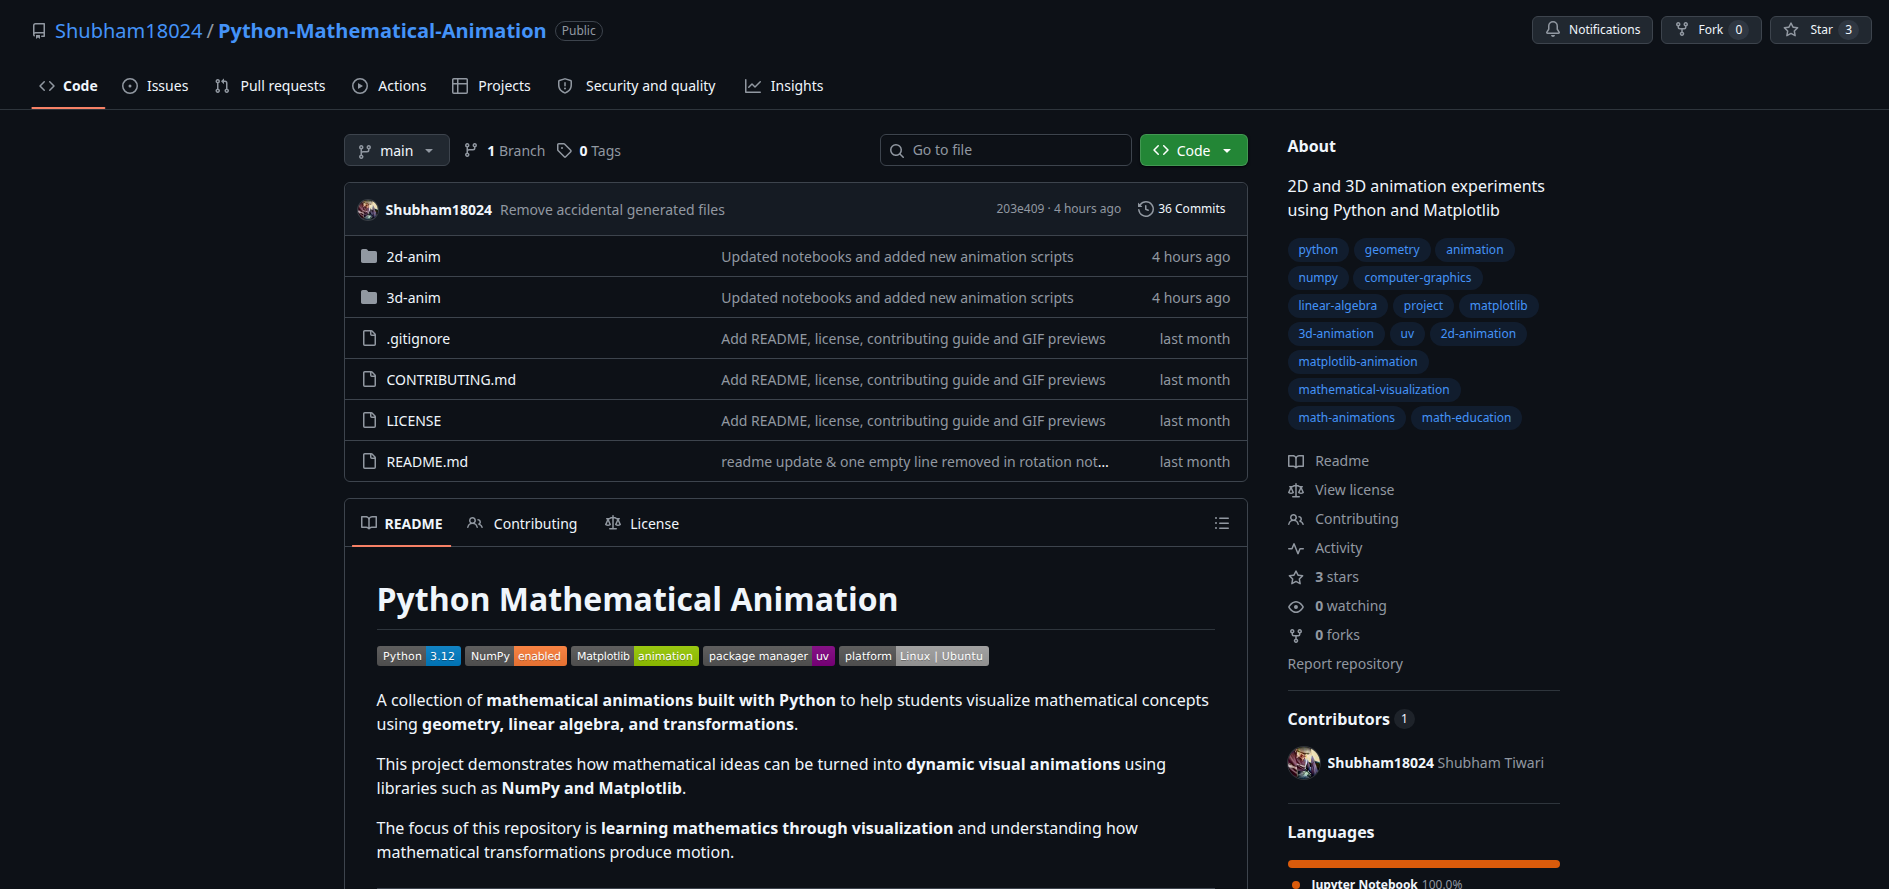
\includegraphics[width=0.98\textwidth]{GITHUB.png}}
    
    \caption{The project's official GitHub repository landing page.}
    \label{fig:github_repo}
\end{figure}

% ------------------------------------------------------------------------------
% APPENDIX B: PROOF OF PUBLICATION
% ------------------------------------------------------------------------------
\chapter{Proof of Publication}
\label{app:acceptance_letter}

The findings and introductory methodologies of this project have been formally accepted for academic publication. The official acceptance letter from \textbf{AkiNik Publications} confirming the publication of the chapter titled \textit{"Introduction: Escaping the Static Chalkboard"} in the edited book \textit{Research Trends in Mathematics and Statistics (Volume - 35)} is attached below.
\begin{figure}[htbp]
    \centering
    % The framebox adds a highly professional thin black border around the white PDF page
    \setlength{\fboxsep}{0pt}
    \fbox{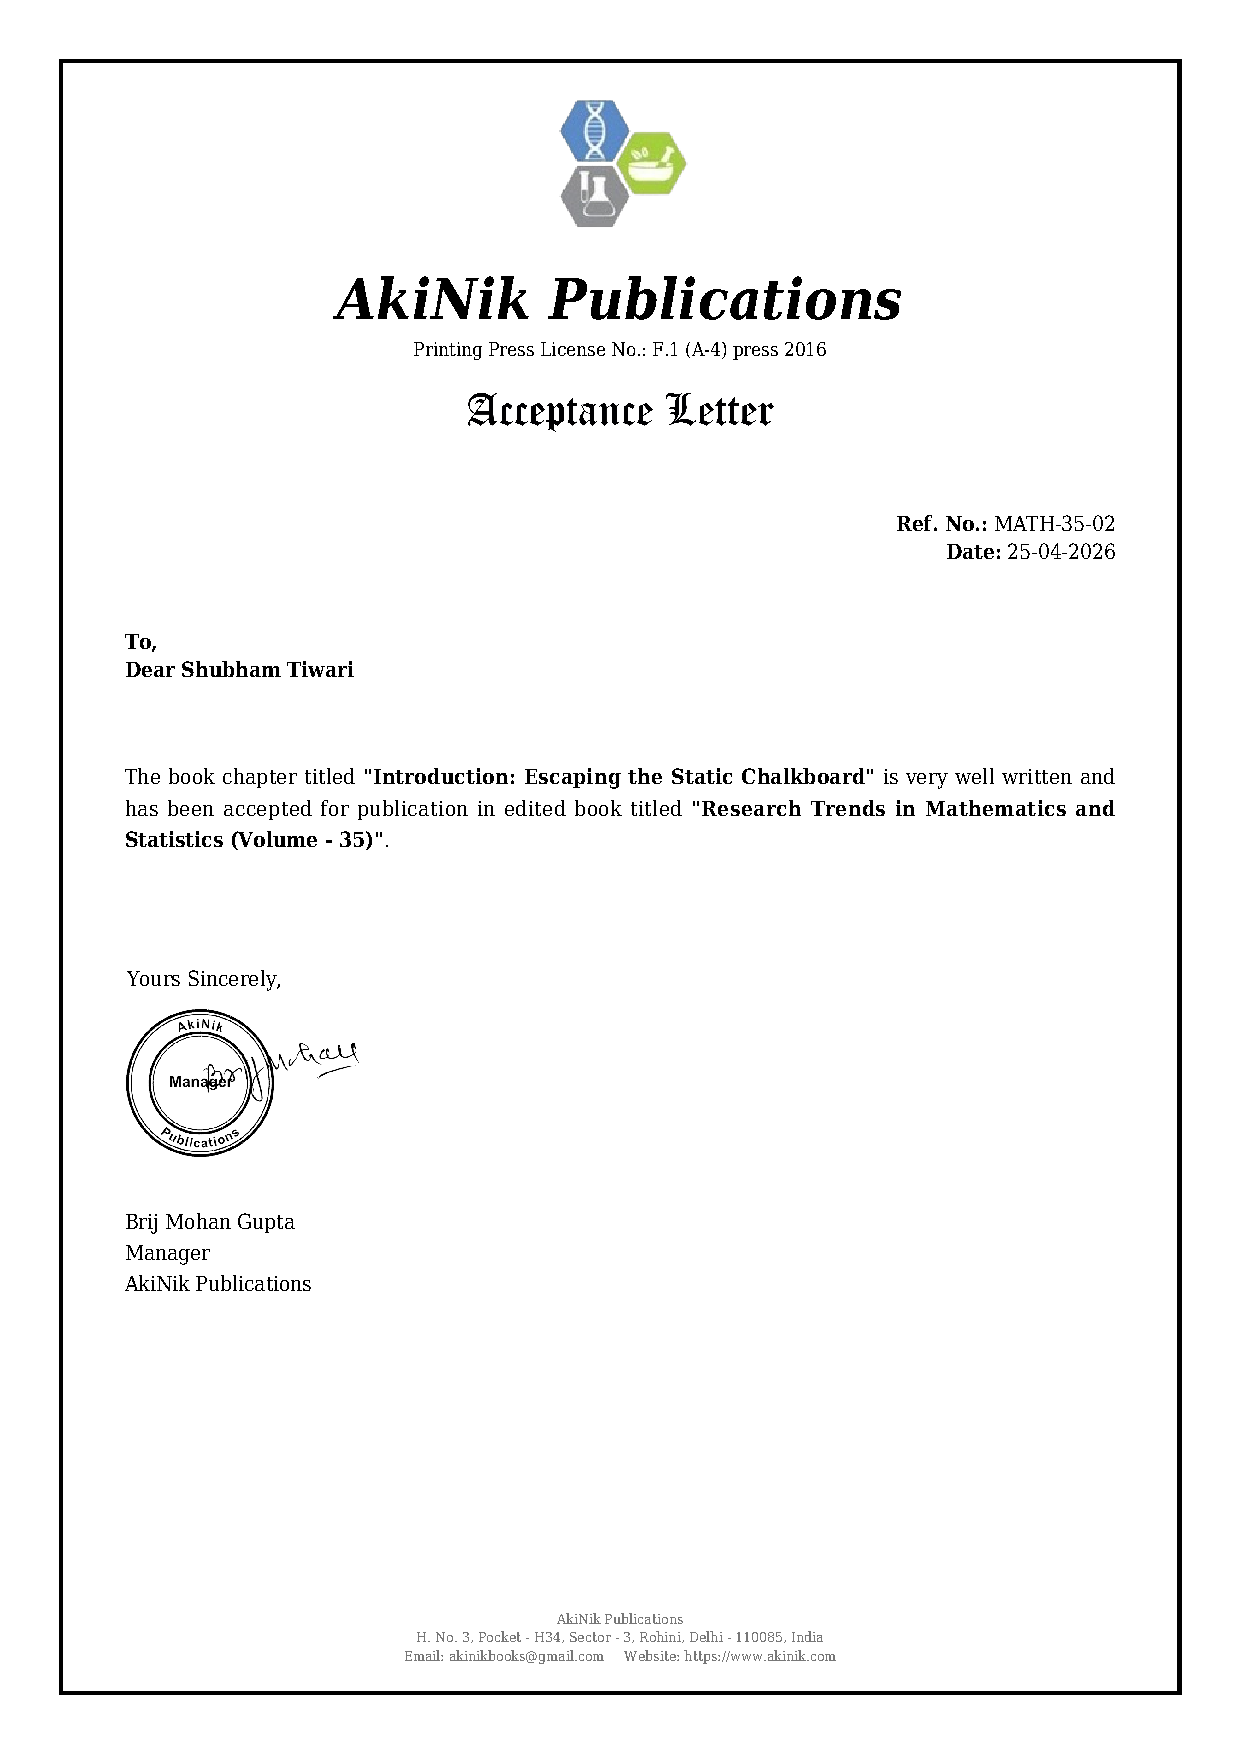
\includegraphics[width=0.85\textwidth]{Acceptance_letter.pdf}}
    
    \caption{Official publication acceptance letter from AkiNik Publications (Ref. No.: MATH-35-02).}
    \label{fig:publisher_proof}
\end{figure}

% =========================================================
% APPENDIX C
% =========================================================
\chapter{Conference Presentation Certificate}
\label{app:conference}

This project was formally presented at the \textit{International Conference on Scientific Computing and its Applications (SCA-2026)} at South Asian University, and the official certificate of paper presentation is attached below.

\vspace{1cm}

\begin{figure}[htbp]
    \centering
    % The framebox adds a highly professional thin black border around the white PDF page
    \setlength{\fboxsep}{0pt}
    \fbox{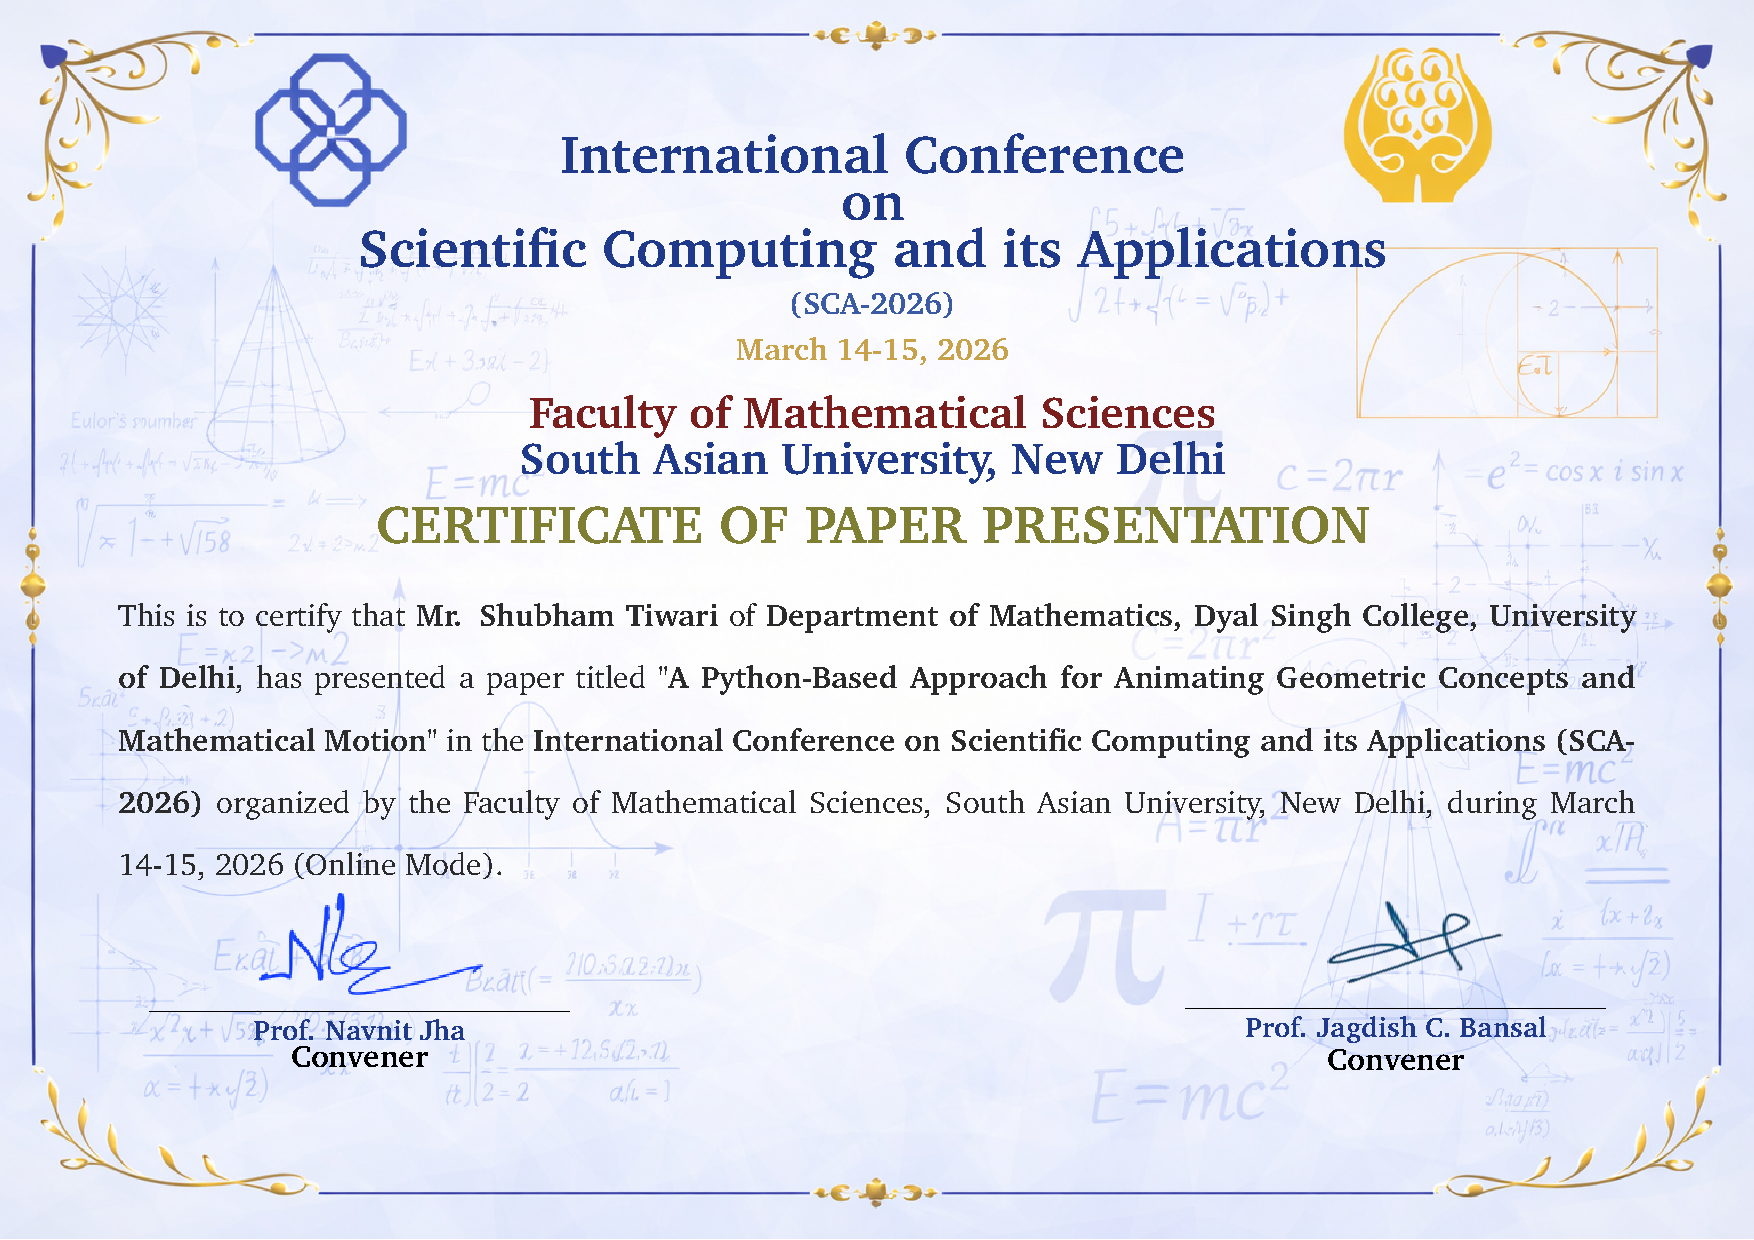
\includegraphics[width=0.85\textwidth]{Participation_certificate.pdf}}
    
    \caption{Official Certificate of Paper Presentation at SCA-2026.}
    \label{fig:conference_certificate}
\end{figure}

% =========================================================
% APPENDIX D
% =========================================================
\chapter{Presentation Slides}
\label{app:ppt}

This appendix contains selected slides from the presentation of this project.

\vspace{0.5cm}

\begin{figure}[htbp]
    \centering
    % Box 1 (Top Left)
    \begin{subfigure}[b]{0.45\textwidth}
        \centering
        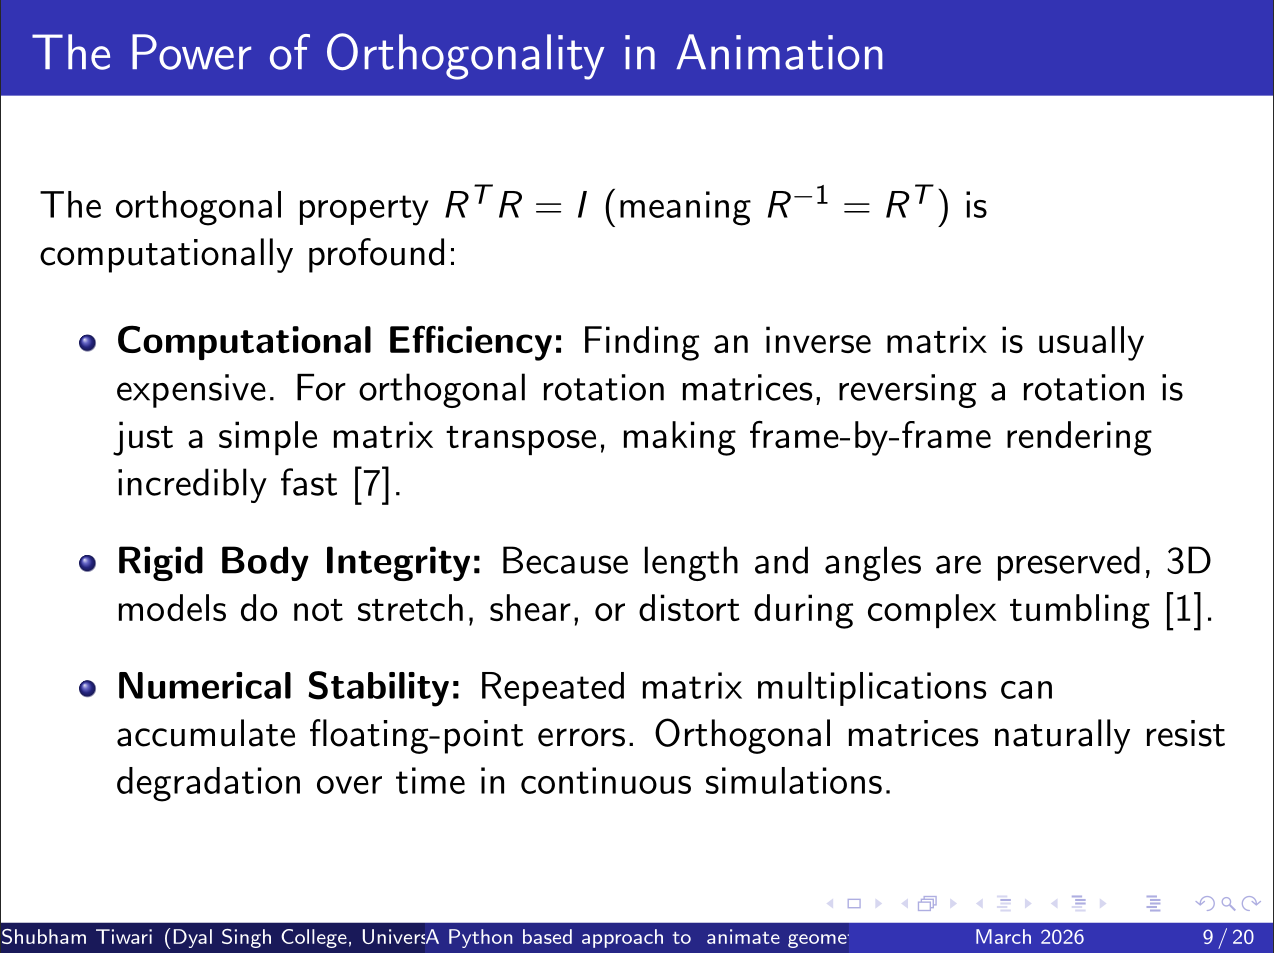
\includegraphics[width=\linewidth]{ppt_1.png}
        \caption{Slide 1: The Power of Orthogonality.}
    \end{subfigure}
    \hfill
    % Box 2 (Top Right)
    \begin{subfigure}[b]{0.45\textwidth}
        \centering
        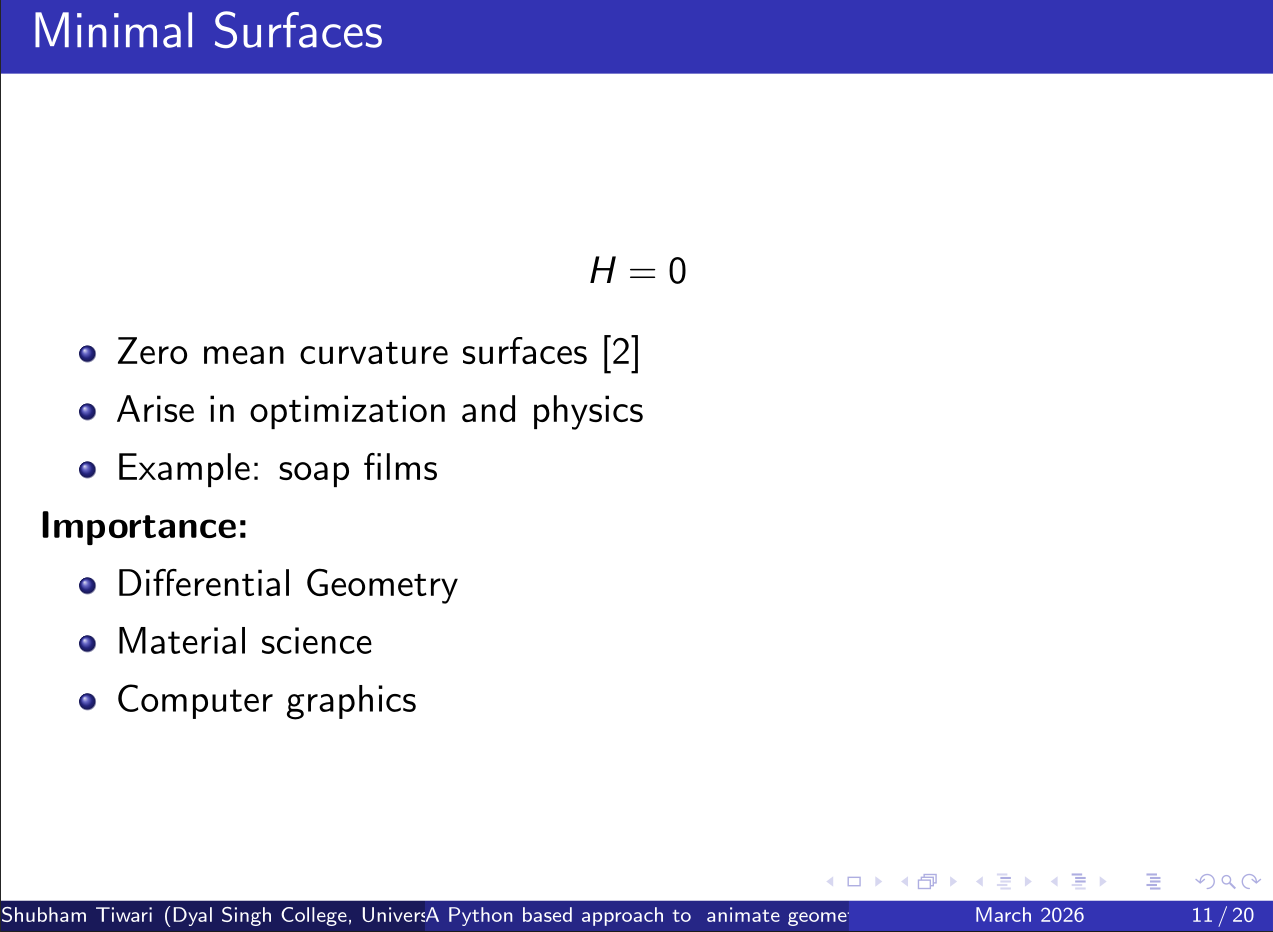
\includegraphics[width=\linewidth]{ppt_2.png}
        \caption{Slide 2: Minimal Surfaces.}
    \end{subfigure}

    \vspace{0.5cm} % Space between rows

    % Box 3 (Bottom Left)
    \begin{subfigure}[b]{0.45\textwidth}
        \centering
        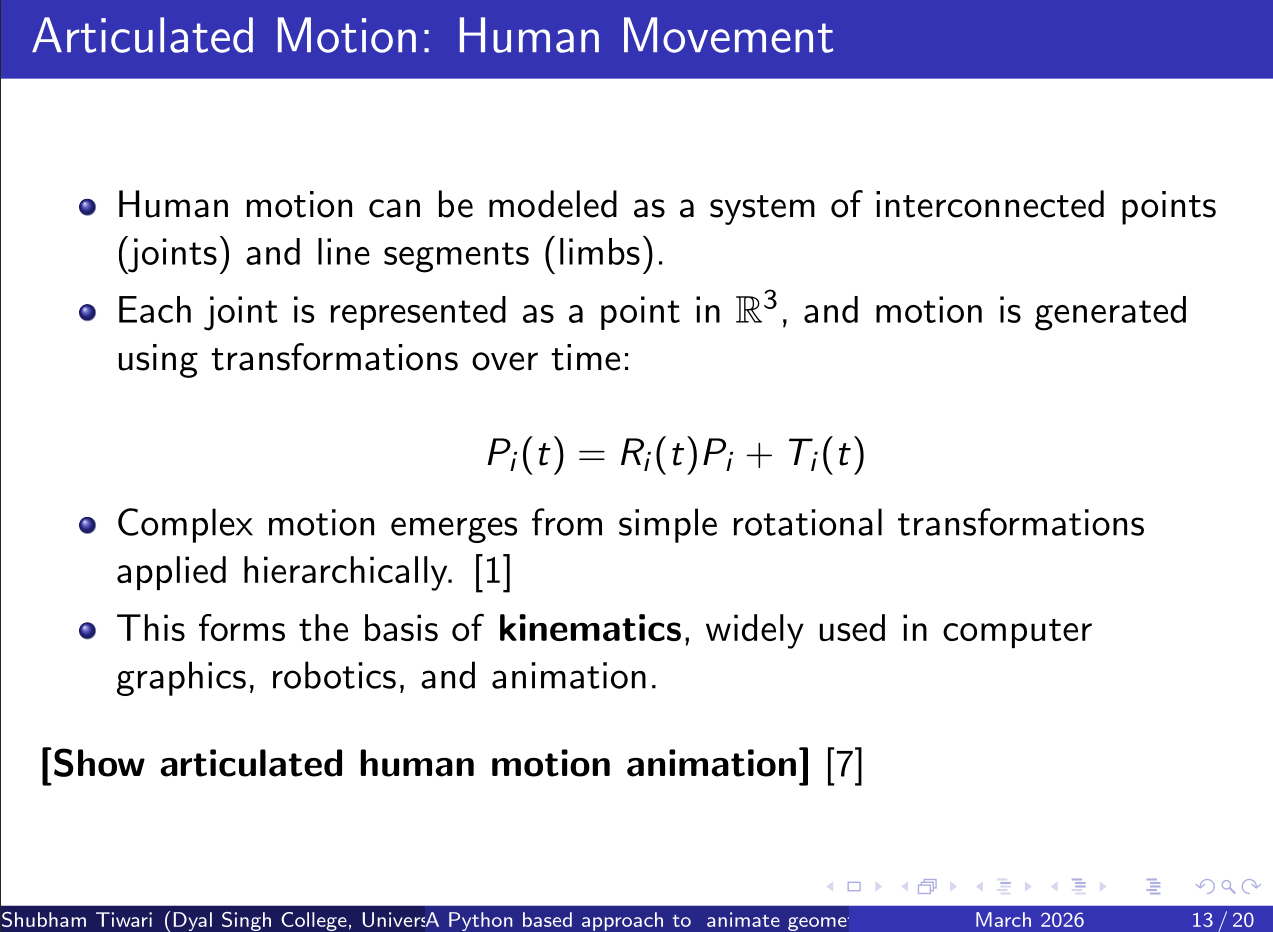
\includegraphics[width=\linewidth]{ppt_3.png}
        \caption{Slide 3: Human Articulated Motion.}
    \end{subfigure}
    \hfill
    % Box 4 (Bottom Right)
    \begin{subfigure}[b]{0.45\textwidth}
        \centering
        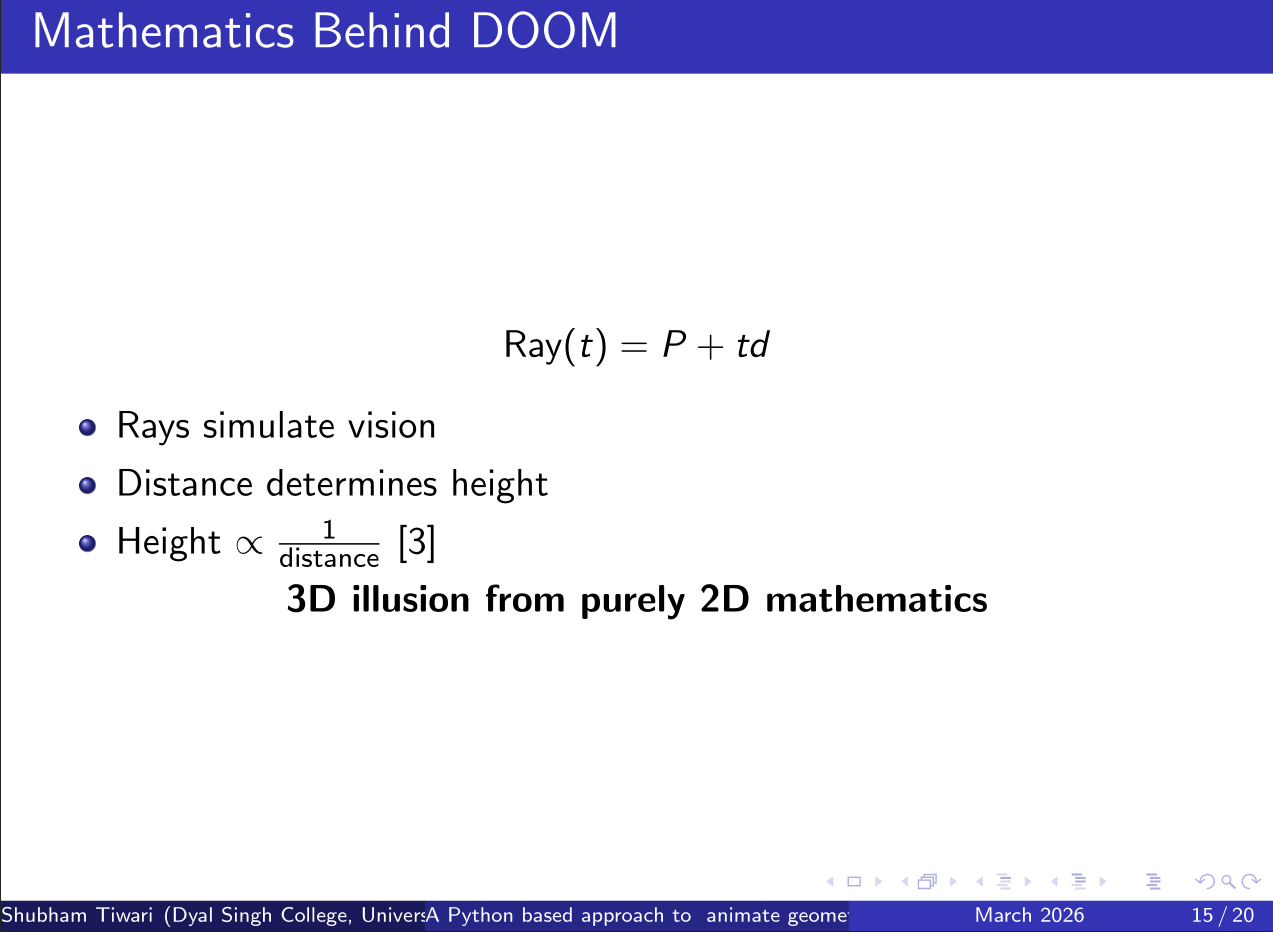
\includegraphics[width=\linewidth]{ppt_4.png}
        \caption{Slide 4: Mathematics behind game 'DOOM'.}
    \end{subfigure}

    \caption{Core slides from the official project presentation.}
    \label{fig:ppt_slides}
\end{figure}

\newpage

% =========================================================
% APPENDIX E
% =========================================================
\chapter{Research Progress \& Monthly Reports}
\label{app:progress}

To ensure rigorous academic development and continuous peer review, formal Monthly Progress Reports (MPRs) were presented to the project supervisor and co-supervisor throughout Semester VIII.
The grid below contains the photographic records of the formal presentations delivered from January 2026 to April 2026.

\begin{figure}[htbp]
    \centering
    % Box 1 (January)
    \begin{subfigure}[b]{0.45\textwidth}
        \centering
        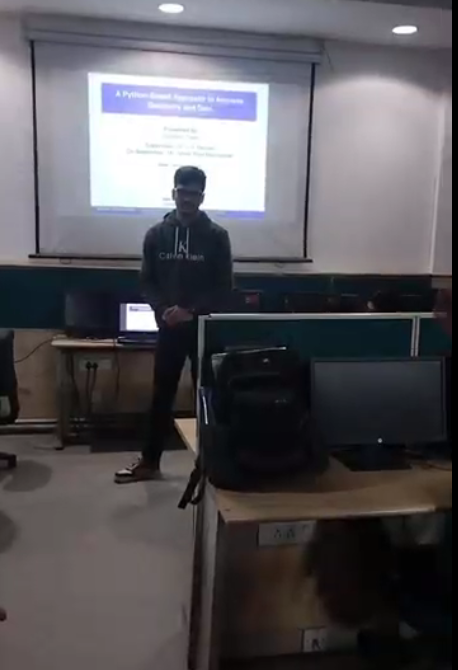
\includegraphics[width=\linewidth]{JAN.png}
        \caption{January 2026 Progress Presentation.}
    \end{subfigure}
    \hfill
    % Box 2 (February)
    \begin{subfigure}[b]{0.45\textwidth}
        \centering
        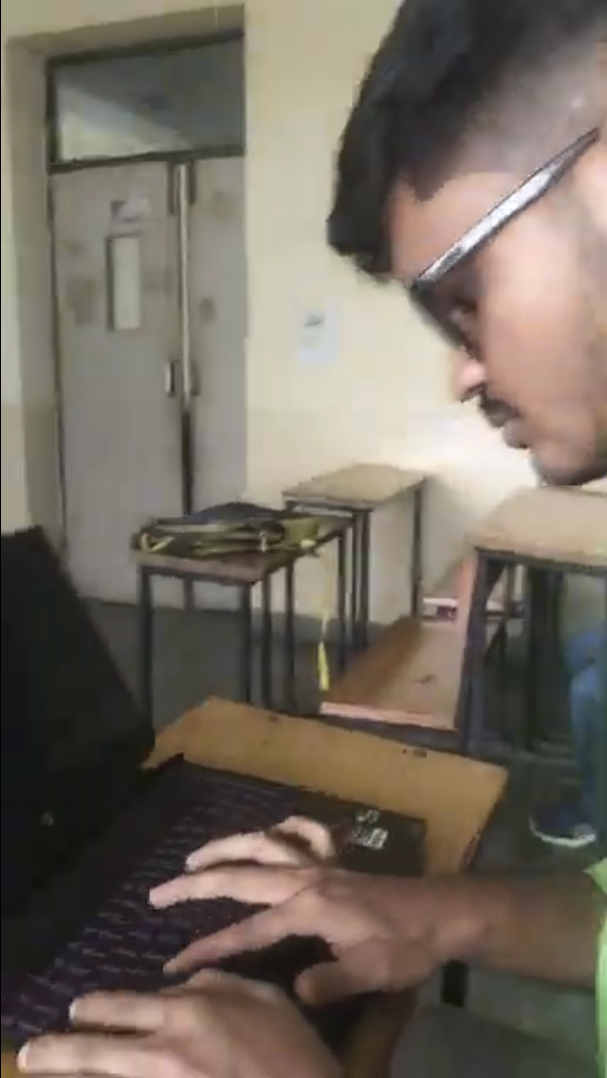
\includegraphics[width=\linewidth]{FEB.png}
        \caption{February 2026 Progress Presentation.}
    \end{subfigure}

    \vspace{0.5cm} % Space between rows

    % Box 3 (March)
    \begin{subfigure}[b]{0.45\textwidth}
        \centering
        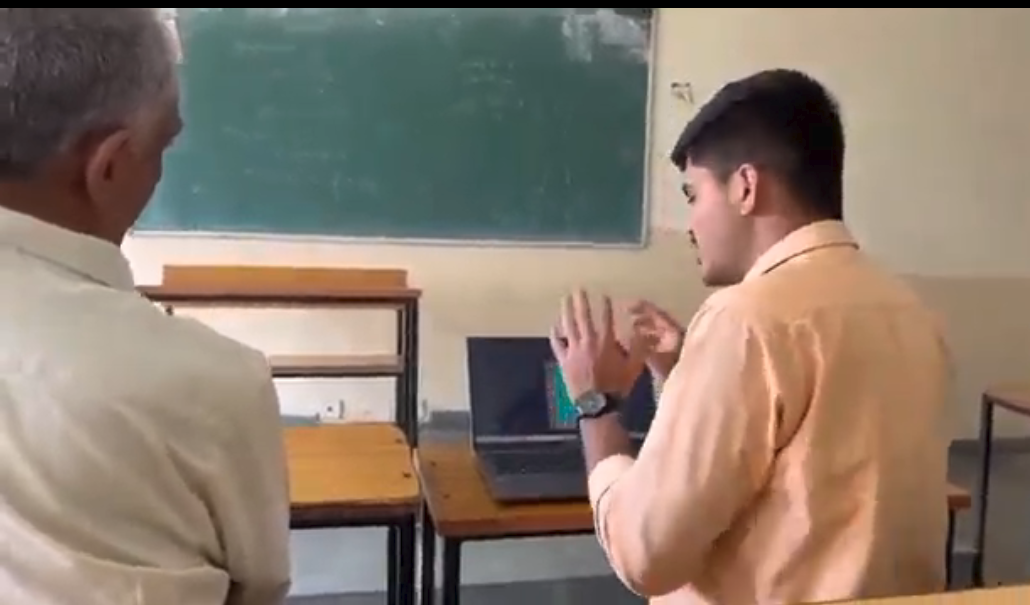
\includegraphics[width=\linewidth]{MAR.png}
        \caption{March 2026 Progress Presentation.}
    \end{subfigure}
    \hfill
    % Box 4 (April)
    \begin{subfigure}[b]{0.45\textwidth}
        \centering
        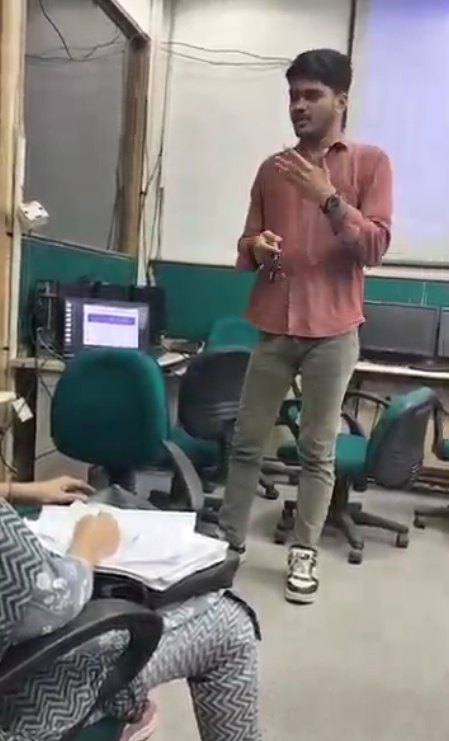
\includegraphics[width=\linewidth]{APR.png}
        \caption{April 2026 Final Review Presentation.}
    \end{subfigure}

    \caption{Monthly progress review presentations delivered during Semester VIII.}
    \label{fig:mpr_grid}
\end{figure}

% =========================================================
% APPENDIX F
% =========================================================
\chapter{Extended Code Snippets}
\label{app:code_snippets}

This appendix contains extended utility functions, environmental setups, and comprehensive execution scripts that drive the core animations discussed in this project report. These snippets are provided for reproducibility and deeper technical inspection.

\section{3D Rigid Body Engine: Rotating Cube}
The following script demonstrates the baseline setup for the 3D canvas and the implementation of $SO(3)$ sequential rotation matrices applied to a discrete vertex array (a cube).

\begin{lstlisting}[language=Python, caption={3D Cube Rotation using Euler Matrices and FuncAnimation}]
import numpy as np
import matplotlib.pyplot as plt
from matplotlib.animation import FuncAnimation
from IPython.display import HTML
plt.rcParams["animation.embed_limit"] = 50  # MB

def base_setup():
    fig, ax = plt.subplots(
        figsize=(6, 6),
        dpi=100,
        subplot_kw={"projection": "3d"}
    )

    ax.set_xlim(-1.5, 1.5)
    ax.set_ylim(-1.5, 1.5)
    ax.set_zlim(-1.5, 1.5)

    ax.set_xlabel("X")
    ax.set_ylabel("Y")
    ax.set_zlabel("Z")

    ax.set_box_aspect([1,1,1])
    ax.view_init(elev=25, azim=30)

    fig.patch.set_facecolor("lightgray") # whole canvas
    ax.set_facecolor("cyan") # background of 3D boxes
    ax.xaxis.pane.set_facecolor("lightblue") # background of x-axis plane
    ax.yaxis.pane.set_facecolor("lightgreen") # background of y-axis plane
    ax.zaxis.pane.set_facecolor("lightyellow") # background of z-axis plane
    ax.grid(False) # turn off grid
    
    return fig, ax

fig, ax = base_setup()

# Cube vertices
P = np.array([
    [-1, 1, 1,-1,-1, 1, 1,-1],
    [-1,-1, 1, 1,-1,-1, 1, 1],
    [-1,-1,-1,-1, 1, 1, 1, 1]
])

# Cube edges
edges = [
    (0,1),(1,2),(2,3),(3,0),
    (4,5),(5,6),(6,7),(7,4),
    (0,4),(1,5),(2,6),(3,7)
]

lines = []
for e in edges:
    line, = ax.plot(
        [P[0,e[0]], P[0,e[1]]],
        [P[1,e[0]], P[1,e[1]]],
        [P[2,e[0]], P[2,e[1]]],
        color='blue'
    )
    lines.append(line)

def Rx(t):
    return np.array([
        [1,0,0],
        [0,np.cos(t),-np.sin(t)],
        [0,np.sin(t), np.cos(t)]
    ])

def Rz(t):
    return np.array([
        [np.cos(t),-np.sin(t),0],
        [np.sin(t), np.cos(t),0],
        [0,0,1]
    ])

def update(frame):
    theta = frame * 0.04

    R = Rz(theta) @ Rx(theta)
    P_rot = R @ P

    for line, edge in zip(lines, edges):
        i, j = edge
        line.set_data(
            [P_rot[0,i], P_rot[0,j]],
            [P_rot[1,i], P_rot[1,j]]
        )
        line.set_3d_properties(
            [P_rot[2,i], P_rot[2,j]]
        )

    ax.set_title(f"Rigid Body Rotation (Cube)\nAngle={theta:.2f} rad")
    return lines

ani = FuncAnimation(fig, update, frames=200, interval=60, blit=True)
plt.close(fig)
HTML(ani.to_jshtml())
\end{lstlisting}

\newpage

\section{Multi-Axis Spherical Rotations}
This script utilizes a meshgrid approach to generate parametric spheres and visualizes simultaneous isolated rotations across the X, Y, and Z axes using a multi-subplot 3D architecture.

\begin{lstlisting}[language=Python, caption={Simultaneous Multi-Axis Parametric Sphere Rotation}]
import numpy as np
import matplotlib.pyplot as plt
from matplotlib.animation import FuncAnimation
from IPython.display import HTML

# SPHERE PARAMETERS
r = 1

theta = np.linspace(0, np.pi, 30)
phi = np.linspace(0, 2*np.pi, 30)

Theta, Phi = np.meshgrid(theta, phi)

# Spherical to Cartesian mapping
X = r * np.sin(Theta) * np.cos(Phi)
Y = r * np.sin(Theta) * np.sin(Phi)
Z = r * np.cos(Theta)

# Rotation functions
def rotate_x(x, y, z, angle):
    c = np.cos(angle)
    s = np.sin(angle)
    x_new = x
    y_new = c*y - s*z
    z_new = s*y + c*z
    return x_new, y_new, z_new

def rotate_y(x, y, z, angle):
    c = np.cos(angle)
    s = np.sin(angle)
    x_new = c*x + s*z
    y_new = y
    z_new = -s*x + c*z
    return x_new, y_new, z_new

def rotate_z(x, y, z, angle):
    c = np.cos(angle)
    s = np.sin(angle)
    x_new = c*x - s*y
    y_new = s*x + c*y
    z_new = z
    return x_new, y_new, z_new

# FIGURE SETUP (3 SUBPLOTS)
fig = plt.figure(figsize=(12,4))

ax1 = fig.add_subplot(131, projection="3d")
ax2 = fig.add_subplot(132, projection="3d")
ax3 = fig.add_subplot(133, projection="3d")

def setup_axis(ax):
    ax.set_xlim(-1.5,1.5)
    ax.set_ylim(-1.5,1.5)
    ax.set_zlim(-1.5,1.5)

    ax.set_box_aspect([1,1,1])
    ax.grid(False)
    ax.view_init(elev=25, azim=30)

    ax.set_xlabel("X")
    ax.set_ylabel("Y")
    ax.set_zlabel("Z")

    fig.patch.set_facecolor("lightgray") 
    ax.set_facecolor("cyan") 
    ax.xaxis.pane.set_facecolor("lightblue") 
    ax.yaxis.pane.set_facecolor("lightgreen") 
    ax.zaxis.pane.set_facecolor("lightyellow") 

def update(frame):
    ax1.clear()
    ax2.clear()
    ax3.clear()

    setup_axis(ax1)
    setup_axis(ax2)
    setup_axis(ax3)

    angle = frame * 0.05

    # X rotation
    Xx, Yx, Zx = rotate_x(X, Y, Z, angle)
    ax1.plot_wireframe(Xx, Yx, Zx, color="red")
    ax1.set_title("Rotation about X-axis")

    # Y rotation
    Xy, Yy, Zy = rotate_y(X, Y, Z, angle)
    ax2.plot_wireframe(Xy, Yy, Zy, color="green")
    ax2.set_title("Rotation about Y-axis")

    # Z rotation
    Xz, Yz, Zz = rotate_z(X, Y, Z, angle)
    ax3.plot_wireframe(Xz, Yz, Zz, color="blue")
    ax3.set_title("Rotation about Z-axis")

ani = FuncAnimation(fig, update, frames=200, interval=50)

plt.close(fig)
HTML(ani.to_jshtml())
\end{lstlisting}

\newpage

\section{Topological Geometry: The Cutaway Torus}
This script models a Cutaway Horn Torus, illustrating the application of parametric constraints. It demonstrates how to wrap a 2D meshgrid around a circular axis in 3D space, followed by an affine rotation sequence.

\begin{lstlisting}[language=Python, caption={Parametric Modeling and Rotation of a Cutaway Horn Torus}]
import numpy as np
import matplotlib.pyplot as plt
from matplotlib.animation import FuncAnimation
from IPython.display import HTML

def base_setup():
    fig, ax = plt.subplots(figsize=(6, 6), dpi=100, subplot_kw={"projection": "3d"})
    # Environment setup abstracted for brevity (see previous scripts)
    return fig, ax

fig, ax = base_setup()

# TORUS PARAMETERS
r = 1 # radius of torus tube
R = 1 # distance from center to tube center (Horn Torus when r=R)

THETA = np.linspace(0, np.pi, 30) # polar angle (0 to pi creates the cutaway)
PHI = np.linspace(0, 2*np.pi, 30) # azimuthal angle (0 to 2pi)

Theta, Phi = np.meshgrid(THETA, PHI)

# SPHERICAL to CARTESIAN
X = (R + r * np.cos(Theta)) * np.cos(Phi)
Y = (R + r * np.cos(Theta)) * np.sin(Phi)
Z = r * np.sin(Theta)   

# ROTATION FUNCTIONS
def rotate_x(x, y, z, angle):
    cos = np.cos(angle)
    sin = np.sin(angle)
    return x, cos*y - sin*z, sin*y + cos*z

def update(frame):
    ax.clear()
    ax.set_xlim(-2.5,2.5)
    ax.set_ylim(-2.5,2.5)
    ax.set_zlim(-2.5,2.5)
    ax.grid(False) 
    ax.set_box_aspect([1,1,1])
    ax.view_init(elev=25, azim=60)

    angle = frame * 0.05
    Xr, Yr, Zr = rotate_x(X, Y, Z, angle)

    ax.plot_wireframe(Xr, Yr, Zr, color="magenta")
    ax.set_title(f"Rigid Body Rotation (Cutaway Horn Torus)\nAngle={angle:.2f} rad")

ani = FuncAnimation(fig, update, frames=200, interval=50)
plt.close(fig)
HTML(ani.to_jshtml())
\end{lstlisting}

\newpage

\section{Differential Topology: Boy's Surface}
Boy's surface is a complex, self-intersecting immersion of the real projective plane ($RP^2$) into $R^3$. The code requires the evaluation of advanced spherical harmonic parameterizations to render the surface accurately before applying rigid body rotations.

\begin{lstlisting}[language=Python, caption={Mathematical Immersion and Rendering of Boy's Surface}]
import numpy as np
import matplotlib.pyplot as plt
from matplotlib.animation import FuncAnimation
from IPython.display import HTML

fig, ax = plt.subplots(figsize=(8,8), subplot_kw={"projection": "3d"})

# PARAMETRIC DOMAIN
U = np.linspace(0, np.pi, 80)
V = np.linspace(0, 2*np.pi, 80)
U, V = np.meshgrid(U, V)

# BOY SURFACE PARAMETRIZATION
X = np.cos(U) * np.sin(V) - np.sin(U) * np.sin(2*V)
Y = np.sin(U) * np.sin(V) + np.cos(U) * np.sin(2*V)
Z = np.cos(V) + np.cos(2*U)

# Normalize scale to prevent bounding box clipping
scale = np.max(np.abs([X,Y,Z]))
X /= scale
Y /= scale
Z /= scale

def rotate_y(x, y, z, angle):
    return np.cos(angle)*x + np.sin(angle)*z, y, -np.sin(angle)*x + np.cos(angle)*z

def rotate_x(x, y, z, angle):
    return x, np.cos(angle)*y - np.sin(angle)*z, np.sin(angle)*y + np.cos(angle)*z

def update(frame):
    ax.clear()
    ax.grid(False)
    ax.set_box_aspect([1,1,1])
    ax.view_init(elev=30, azim=40)

    angle = frame * 0.05

    # Apply dual-axis rotation
    Xr, Yr, Zr = rotate_y(X, Y, Z, angle)
    Xr, Yr, Zr = rotate_x(Xr, Yr, Zr, angle*0.6)

    limit = 1.4
    ax.set_xlim(-limit,limit)
    ax.set_ylim(-limit,limit)
    ax.set_zlim(-limit,limit)

    # Render as a solid continuous surface using colormaps
    ax.plot_surface(Xr, Yr, Zr, cmap="viridis", edgecolor="none", alpha=0.9)
    ax.set_title("Boy's Surface (Projective Plane Immersion)")

ani = FuncAnimation(fig, update, frames=200, interval=50)
plt.close(fig)
HTML(ani.to_jshtml())
\end{lstlisting}

\newpage

\section{Combined Kinematics: Translation and Rotation}
This script represents the most complex physical modeling in the project, computing translation vectors ($T$) and rotation matrices ($R$) simultaneously across multiple independent objects.

\begin{lstlisting}[language=Python, caption={Simultaneous Orbit, Translation, and Rotation of Multiple Solids}]
import numpy as np
import matplotlib.pyplot as plt
from matplotlib.animation import FuncAnimation
from mpl_toolkits.mplot3d.art3d import Poly3DCollection
from IPython.display import HTML

fig = plt.figure()
ax = fig.add_subplot(111, projection="3d")

# Cube vertices and topological faces
P = np.array([
    [-1, 1, 1,-1,-1, 1, 1,-1],
    [-1,-1, 1, 1,-1,-1, 1, 1],
    [-1,-1,-1,-1, 1, 1, 1, 1]
])

faces = [
    [0,1,2,3], [4,5,6,7], [0,1,5,4], 
    [1,2,6,5], [2,3,7,6], [3,0,4,7]
]

def Rx(t):
    return np.array([[1,0,0], [0,np.cos(t),-np.sin(t)], [0,np.sin(t), np.cos(t)]])

def Rz(t):
    return np.array([[np.cos(t),-np.sin(t),0], [np.sin(t), np.cos(t),0], [0,0,1]])

def draw_cube(P_transformed, color):
    face_polygons = []
    for f in faces:
        face = [[P_transformed[0,i], P_transformed[1,i], P_transformed[2,i]] for i in f]
        face_polygons.append(face)

    cube = Poly3DCollection(face_polygons, facecolors=color, edgecolors="black", alpha=0.7)
    ax.add_collection3d(cube)

def update(frame):
    ax.clear()
    ax.set_xlim(-6,6)
    ax.set_ylim(-6,6)
    ax.set_zlim(-6,6)
    ax.set_box_aspect([1,1,1])
    ax.grid(False)

    theta = frame * 0.04
    R = Rz(theta) @ Rx(theta)

    # Cube 1: Stationary Center Rotation
    P1 = R @ P
    draw_cube(P1, "cyan")

    # Cube 2: Linear Translation + Rotation
    tx = np.sin(theta) * 4
    T1 = np.array([tx,0,0])
    P2 = R @ P + T1[:,None] # Broadcasting translation vector
    draw_cube(P2, "orange")

    # Cube 3: Orbital Motion + Rotation
    tx2 = np.cos(theta) * 4
    ty2 = np.sin(theta) * 4
    T2 = np.array([tx2,ty2,0])
    P3 = R @ P + T2[:,None]
    draw_cube(P3, "magenta")

    ax.set_title("Rotation + Translation (Multiple Cubes)")

ani = FuncAnimation(fig, update, frames=200, interval=50)
plt.close(fig)
HTML(ani.to_jshtml())
\end{lstlisting}

\newpage

\section{Articulated Kinematics: Human Motion Simulation}
This script demonstrates hierarchical coordinate transformations. By defining a root node (the hip) and chaining rotation matrices ($R_x$) down through the limbs, the code successfully simulates a walking bipedal figure using pure vector addition and trigonometric oscillation.

\begin{lstlisting}[language=Python, caption={Hierarchical Kinematics of an Articulated Human Figure}]
import numpy as np
import matplotlib.pyplot as plt
from matplotlib.animation import FuncAnimation
from IPython.display import HTML

fig = plt.figure()
ax = fig.add_subplot(111, projection='3d')

ax.set_xlim(-3,3)
ax.set_ylim(-3,3)
ax.set_zlim(0,6)
ax.set_box_aspect([1,1,1])
ax.grid(False)

# Rotation around x axis (for limb swing)
def Rx(theta):
    return np.array([
        [1,0,0],
        [0,np.cos(theta),-np.sin(theta)],
        [0,np.sin(theta), np.cos(theta)]
    ])

# Function to draw limb vectors
def draw_limb(start, vec):
    end = start + vec
    ax.plot(
        [start[0],end[0]], [start[1],end[1]], [start[2],end[2]],
        color="black", linewidth=3
    )
    return end

def update(frame):
    ax.clear()
    ax.set_xlim(-3,3)
    ax.set_ylim(-3,3)
    ax.set_zlim(0,6)
    ax.set_box_aspect([1,1,1])
    ax.grid(False)

    t = frame * 0.08

    # Body root
    hip = np.array([0,0,2])

    # Torso and Head
    torso_vec = np.array([0,0,2])
    neck = draw_limb(hip, torso_vec)
    ax.scatter(neck[0], neck[1], neck[2]+0.5, s=200, color="orange")
    shoulder = neck

    # Arm swing (Oscillating)
    arm_angle = np.sin(t)
    R_arm = Rx(arm_angle)
    
    # Left Arm
    upper_arm = R_arm @ np.array([0,0,-1.2])
    elbow = draw_limb(shoulder + np.array([0.4,0,0]), upper_arm)
    lower_arm = R_arm @ np.array([0,0,-1])
    draw_limb(elbow, lower_arm)

    # Right Arm (Inverse Oscillation)
    R_arm2 = Rx(-arm_angle)
    upper_arm2 = R_arm2 @ np.array([0,0,-1.2])
    elbow2 = draw_limb(shoulder + np.array([-0.4,0,0]), upper_arm2)
    lower_arm2 = R_arm2 @ np.array([0,0,-1])
    draw_limb(elbow2, lower_arm2)

    # Leg swing
    leg_angle = np.sin(t)
    
    # Left Leg
    R_leg = Rx(-leg_angle)
    upper_leg = R_leg @ np.array([0,0,-1.5])
    knee = draw_limb(hip + np.array([0.3,0,0]), upper_leg)
    lower_leg = R_leg @ np.array([0,0,-1.5])
    draw_limb(knee, lower_leg)

    # Right Leg
    R_leg2 = Rx(leg_angle)
    upper_leg2 = R_leg2 @ np.array([0,0,-1.5])
    knee2 = draw_limb(hip + np.array([-0.3,0,0]), upper_leg2)
    lower_leg2 = R_leg2 @ np.array([0,0,-1.5])
    draw_limb(knee2, lower_leg2)

    ax.set_title("Simple Human Motion (Articulated Figure)")

ani = FuncAnimation(fig, update, frames=200, interval=50)
plt.close(fig)
HTML(ani.to_jshtml())
\end{lstlisting}

\newpage

\section{Stochastic Processes: 2D Random Walk}
This script visualizes a classic discrete stochastic process. By utilizing a random number generator to dictate direction, it animates the continuous path of a particle under Brownian-like motion on a 2D Cartesian plane.

\begin{lstlisting}[language=Python, caption={Discrete 2D Random Walk Simulation}]
import numpy as np
import matplotlib.pyplot as plt
import matplotlib.animation as animation

# Setup figure and axes
fig, axs = plt.subplots()
a = 7
axs.set_xlim(-a, a)
axs.set_ylim(-a, a)
axs.axhline(0, color='black', linewidth=3)   
axs.axvline(0, color='black', linewidth=3) 
axs.set_aspect('equal', adjustable='box')

N = 100 # Total frames

# Path initialization
x, y = [0], [0]
path_line, = axs.plot([], [], 'r-', linewidth=2)

def init():
    x.clear()  
    y.clear()  
    x.append(0)  
    y.append(0)  
    path_line.set_data([], [])
    return path_line,

def update(frame):
    xold = x[frame]
    yold = y[frame]
    
    # Stochastic step logic
    rnd = np.random.randint(1, 5)
    if rnd == 1:
        xnew, ynew = xold + 1, yold
    elif rnd == 2:
        xnew, ynew = xold - 1, yold
    elif rnd == 3:
        xnew, ynew = xold, yold + 1
    else:
        xnew, ynew = xold, yold - 1
        
    x.append(xnew)
    y.append(ynew)
    path_line.set_data(x, y)
    return path_line,

ani = animation.FuncAnimation(fig, update, frames=N, init_func=init, blit=True, interval=50)

plt.title("Random Walk 2D")
plt.xlabel("x")
plt.ylabel("y")
plt.grid(True)
plt.show()
\end{lstlisting}

\newpage

\section{Metric Space Topology: $L_p$ Norm Unit Balls}
This script dynamically visualizes the morphing topology of unit balls in $\mathbb{R}^2$ under different $L_p$ norms. It includes a specific conditional block to handle the topological limit when $p = \infty$ (the Chebyshev distance).

\begin{lstlisting}[language=Python, caption={Visualizing $L_p$ Unit Balls from $p=1$ to $p=\infty$}]
import numpy as np
import matplotlib.pyplot as plt
import matplotlib.animation as animation

def setup_axes():
    fig, ax = plt.subplots(figsize=(6,6))
    ax.set_xlim(-1.5, 1.5)
    ax.set_ylim(-1.5, 1.5)
    ax.axhline(0, color="black", linewidth=1)
    ax.axvline(0, color="black", linewidth=1)
    ax.set_aspect("equal")
    ax.set_title("Unit Ball in Different Norms on R^2")
    return fig, ax

def lp_unit_ball(p, num_points=400):
    theta = np.linspace(0, 2*np.pi, num_points)

    # Limit Condition for p = infinity (Chebyshev distance)
    if p == np.inf:
        n = num_points // 4
        x = np.concatenate([
            np.linspace(-1, 1, n),
            np.ones(n),
            np.linspace(1, -1, n),
            -np.ones(n)
        ])
        y = np.concatenate([
            np.ones(n),
            np.linspace(1, -1, n),
            -np.ones(n),
            np.linspace(-1, 1, n)
        ])
        return x[:num_points], y[:num_points]

    # Standard parametric generation for finite p
    x = np.sign(np.cos(theta)) * (np.abs(np.cos(theta)) ** (2/p))
    y = np.sign(np.sin(theta)) * (np.abs(np.sin(theta)) ** (2/p))
    return x, y

def update(frame):
    ax.clear()

    p_index = frame // points_per_norm
    t_index = frame % points_per_norm
    current_p = p_values[p_index]

    x, y = lp_unit_ball(current_p)
    ax.plot(x, y, 'r', linewidth=2)

    ax.set_title(f"Unit Ball in L_p for p = {current_p}")
    ax.set_xlim(-1.5, 1.5)
    ax.set_ylim(-1.5, 1.5)
    ax.set_aspect("equal")
    ax.axhline(0, color="black", linewidth=1)
    ax.axvline(0, color="black", linewidth=1)

    ax.plot(x[t_index], y[t_index], 'bo', markersize=8)
    return []

p_values = [1,2,3,4,5,6,7,8,9,10,np.inf]
points_per_norm = 300
total_frames = len(p_values) * points_per_norm

fig, ax = setup_axes()
ani = animation.FuncAnimation(fig, update, frames=total_frames, interval=20)
plt.show()
\end{lstlisting}

%=====================================================================

% =========================================================
% APPENDIX G
% =========================================================
\chapter{Plagiarism Originality Report}
\label{app:plagiarism}
% Inserts the first 2 pages of the Plagiarism PDF, scaled to fit the margins
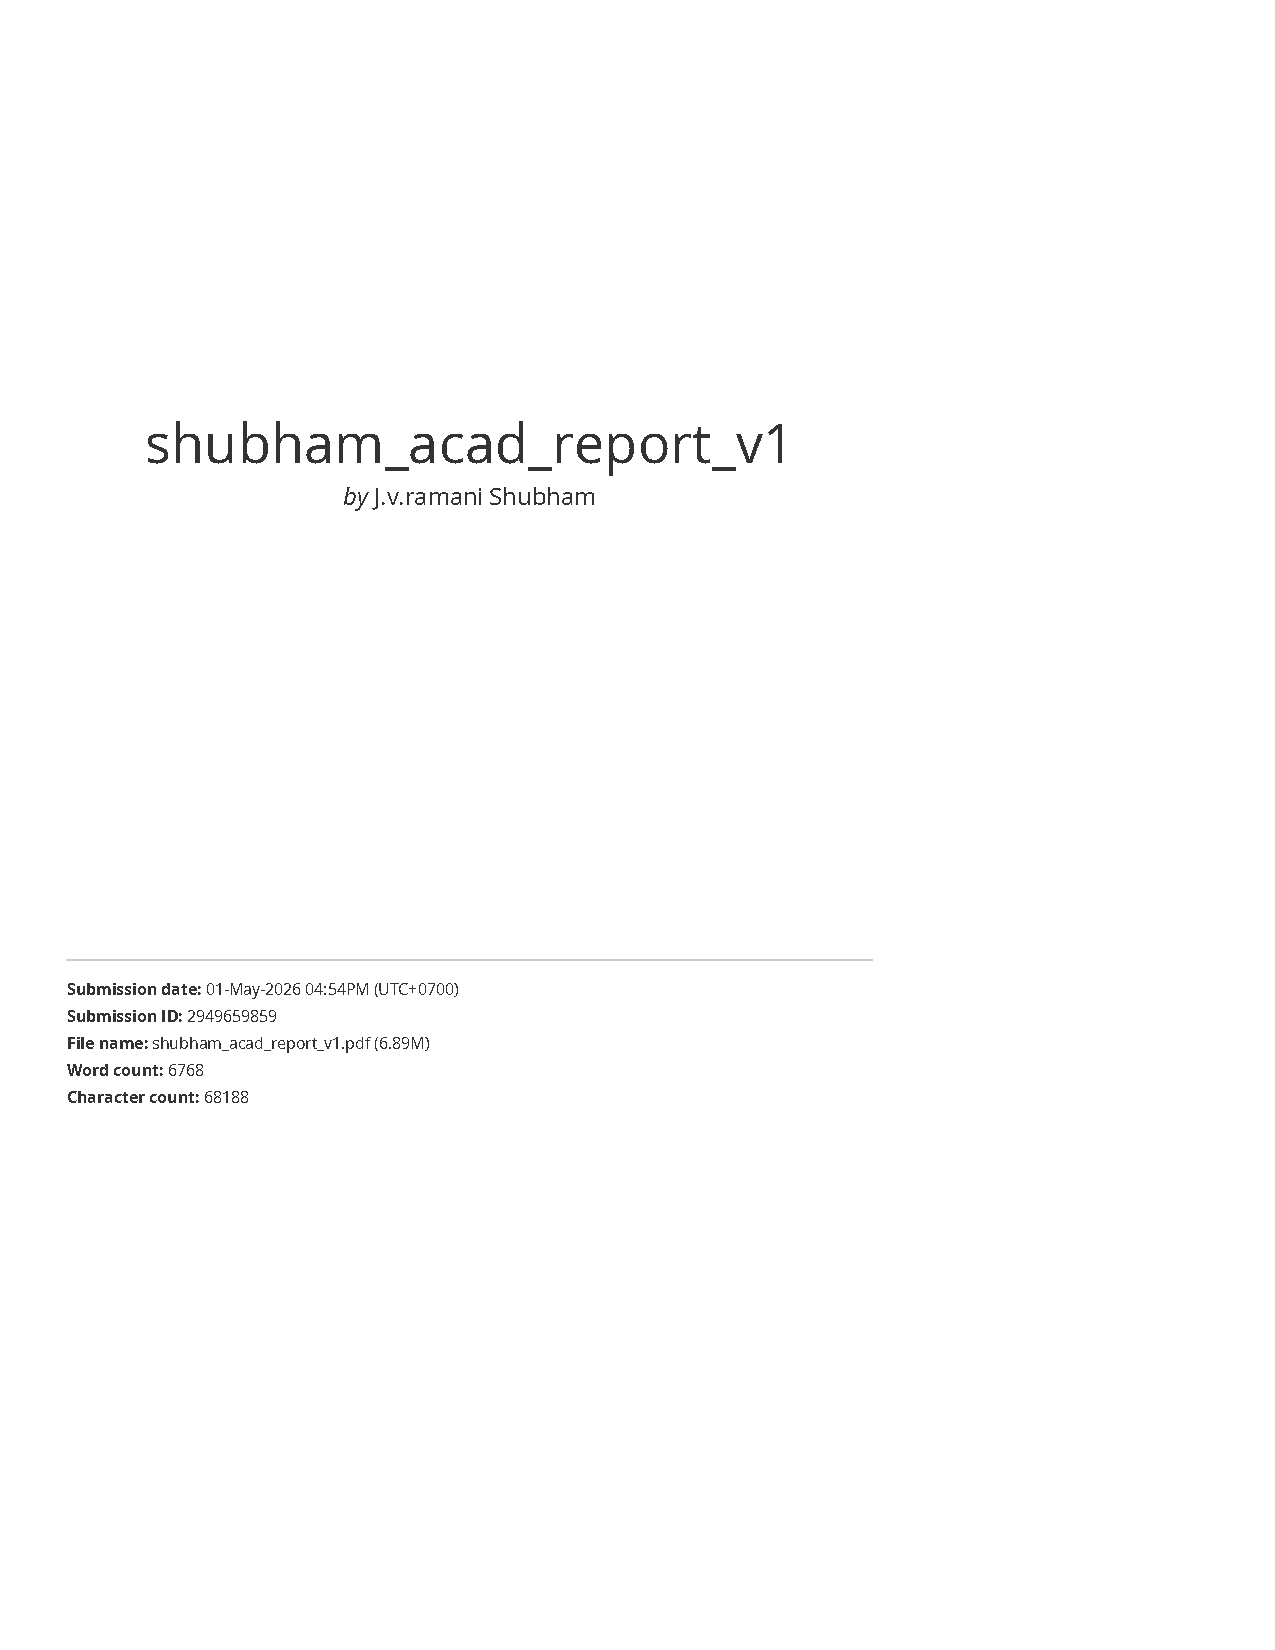
\includepdf[pages={1-2}, scale=0.85, pagecommand={\thispagestyle{fancy}}]{palagarism_Report_turnitin.pdf} 

% =========================================================
% APPENDIX H
% =========================================================
\chapter{AI Writing Overview}
\label{app:ai_report}
% Inserts the first 2 pages of the AI PDF, scaled to fit the margins
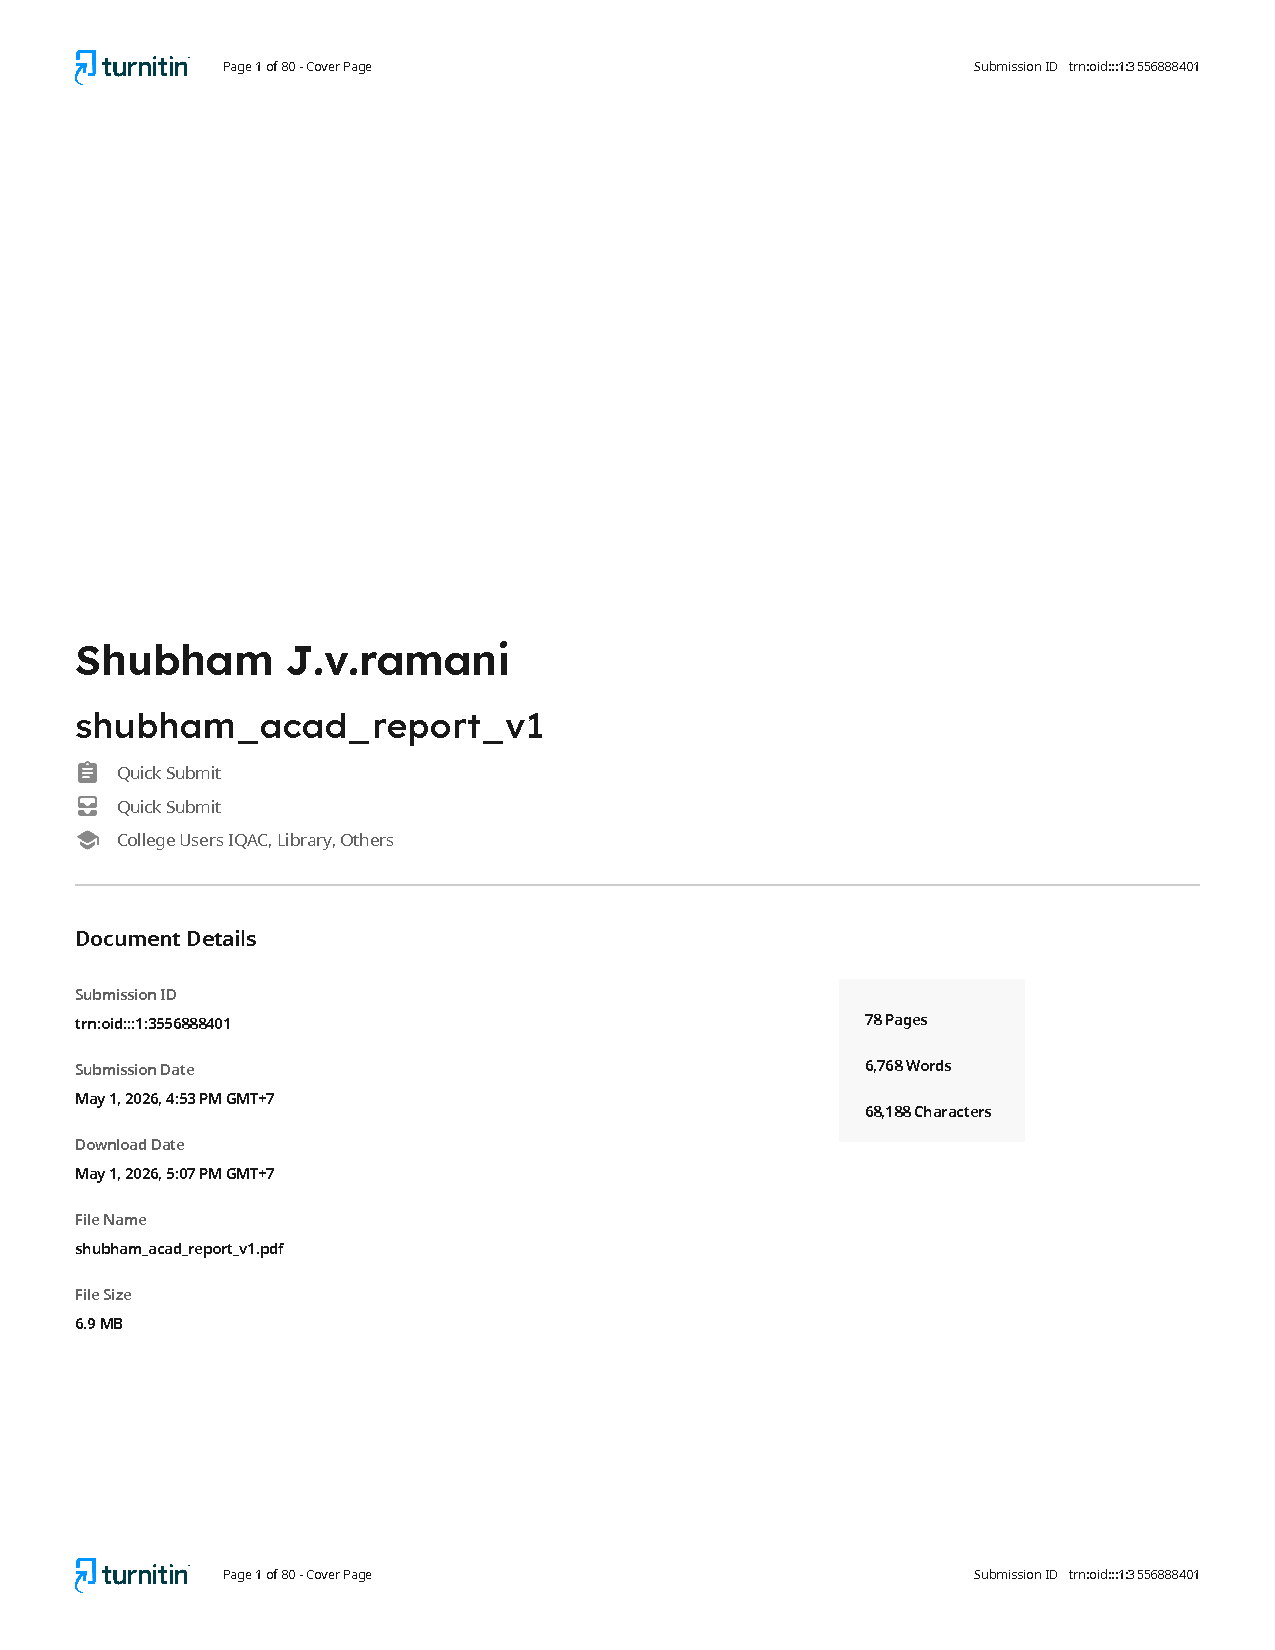
\includepdf[pages={1-2}, scale=0.85, pagecommand={\thispagestyle{fancy}}]{ai_report_turnitin.pdf}

%=====================================================================

\end{document}